\documentclass[11pt,oneside,openany]{book}

\usepackage{natbib}
\usepackage[french]{babel}
\usepackage[utf8]{inputenc}
\usepackage[T1]{fontenc}
\usepackage{lmodern}

\usepackage{amssymb, amsmath, amsthm, multirow, float, bm}
\usepackage{graphicx, xcolor, enumitem, tikz}
\usetikzlibrary{arrows.meta, calc}
\usepackage{subcaption,listings}
\usepackage[colorlinks=true, allcolors=blue]{hyperref}
\usepackage{bookmark}

\providecommand{\Y}{Y}
\newtheorem{remarque}{Remarque}
\newtheorem{theorem}{Théorème}
\newtheorem{corol}[theorem]{Corollaire}
%\newtheorem{exemple}{Exemple}[chapter]
\newtheorem{defn}{Définition}[chapter]


%Raccourcis mathématiques

\newcommand{\esp}{\mathbb{E}}
\newcommand{\var}{\mathbb{V}\text{ar}}
\newcommand{\cov}{\mathbb{C}\text{ov}}
\newcommand{\corr}{\mathbb{C}\text{orr}}
\newcommand{\prob}{\mathbb{P}}
\newcommand{\N}{\mathcal{N}}
\newcommand{\iid}{\overset{iid}{\sim}}


\def\I{\mathbb{I}}
\def\R{\mathbb{R}}
\def\P{{\mathbb P}}


%\newcommand{\boldmath}{\boldmath}
\newcommand{\um}{\unboldmath}
\newcommand{\botheta}{\bm\theta}
\newcommand{\boTheta}{\bm\Theta}
\newcommand{\boY}{\bm{Y}}
\newcommand{\bobeta}{\bm\beta}
\newcommand{\boeps}{\bm\varepsilon}
\newcommand{\boldx}{\bm{x}}
\newcommand{\boldu}{\bm{u}}
\newcommand{\boldA}{\bm{A}}
\newcommand{\boR}{\bm{R}}
\newcommand{\boun}{\bm{1}}
\newcommand{\boz}{\bm{0}}
\newcommand{\bolambda}{\bm\lambda}
\newcommand{\bov}{\bm{v}}
\newcommand{\boalpha}{\bm\alpha}
\newcommand{\bo}[1]{{\bm{#1}}}
\newcommand{\boX}{\bm{X}}
\newcommand{\boV}{\bm{V}}
\newcommand{\hbobeta}{\widehat{\bobeta}}
\newcommand{\hboeps}{\widehat{\boeps}}
\newcommand{\hY}{\widehat{\boY}}
\newcommand{\boH}{\bm{H}}
\newcommand{\boI}{\bm{\I}}
\newcommand{\eproof}{\hfill$\sqcap\!\!\!\!\sqcup$}
\newcommand{\bou}{\bm u}


\DeclareRobustCommand{\vect}[1]{\bm{#1}}
\pdfstringdefDisableCommands{%
  \renewcommand{\vect}[1]{#1}%
} %Symboles programmés pour simplifier le texte

\usepackage{version} % Pour faire un texte troué pour les étudiants
%\includeversion{etudiant}\excludeversion{professeur} %version etudiant
\includeversion{professeur}\excludeversion{etudiants} %version prof
\newcommand{\etudiant}[1]{\begin{etudiants}#1 \end{etudiants}}
\newcommand{\prof}[1]{\begin{professeur}\color{blue} #1 \end{professeur}}


%%% boîte Exemple %%%
\usepackage[framemethod=default]{mdframed}
\definecolor{vertEx}{HTML}{138808} 
\colorlet{vertExemple}{vertEx!90!yellow} 
\mdfdefinestyle{exemplestyle}{%
    topline=false, rightline=false, bottomline=false, leftline=true,  
    linecolor=vertExemple,  
    linewidth=3pt,  
    backgroundcolor=vertExemple!8
}
\newmdtheoremenv[style=exemplestyle]{exemple}{Exemple}[chapter]  
%%% boîte Définition %%%
\definecolor{rougeDef}{rgb}{0.94, 0.30, 0.22}
\mdfdefinestyle{defstyle}{%
    topline=false, rightline=false, bottomline=false, leftline=true,  
    linecolor=rougeDef!80,  
    linewidth=3pt,  
    backgroundcolor=rougeDef!5
}
\newmdtheoremenv[style=defstyle]{proposition}{Proposition}[chapter]  


\renewcommand{\familydefault}{\sfdefault} % Police 
\renewcommand{\baselinestretch}{1.3} % entre 1 et 1.5 d'interligne
\usepackage{geometry} 
\geometry{margin=1in} 

\usepackage{minitoc} % Pour table des matières par chapitres
\mtcselectlanguage{french} % minitoc en français

\definecolor{lb}{rgb}{1.0, 0.22, 0.0}
\newcommand{\bfr}[1]{\textbf{\textcolor{lb}{#1}}} % Pour le texte en gras et en rouge


\title{STT-2100 \\ Régression \\ Université Laval \\[3cm]}
\author{Document collaboratif de: \\
Anne-Sophie Charest \\
Thierry Duchesne \\
Anne-Catherine Favre \\
Christian Genest \\
Emmanuelle Reny-Nolin \\
Véronique Tremblay \\
Audrey-Anne Vallée \\[3cm]}
\date{\ifcase\month\or
  Janvier\or Février\or Mars\or Avril\or Mai\or Juin\or
  Juillet\or Août\or Septembre\or Octobre\or Novembre\or Décembre\fi, \the\year}


\begin{document}
\maketitle

\dominitoc \tableofcontents
\dominilof \listoffigures

% Chapitre 1 - Introduction
\chapter{Introduction} \label{sec:intro}
\minitoc \mtcskip \minilof

\section{Un peu d'histoire}

L'origine du mot \textit{régression} vient de Sir Francis Galton (1822--1911), un scientifique britannique. Cousin de Charles Darwin, Galton était un touche-à-tout intuitif qui fut anthropologue, explorateur, géographe, inventeur, météorologue, généticien, psychométricien et statisticien.
%\footnote{Plus d'informations sur la biographie de Sir Francis Galton sont disponibles à l'adresse \url{http://fr.wikipedia.org/wiki/Francis_Galton}}.
En 1886, en travaillant sur l'hérédité, il s'est intéressé à la taille des enfants par rapport à celle de leurs parents. Il constata que lorsque les parents étaient plus grands que la moyenne, leurs enfants avaient tendance à être plus petits qu'eux et que, inversement, lorsque les parents étaient plus petits que la moyenne leurs enfants tendaient à être plus grands qu'eux. Il publia sa découverte  dans l'article \emph{Regression towards mediocrity in hereditary stature} \citep{Gal:1886}. Il utilisa le terme régression dans le sens où les parents de taille extrême (petits et grands) voient en moyenne la taille de leurs enfants régresser vers la moyenne.

Par extension, on utilise maintenant le terme \textbf{analyse de régression} pour désigner l'étude des relations qui existent entre des variables mesurables à partir d’observations (données) prises sur ces variables.

L'analyse de la relation entre plusieurs variables est toutefois bien plus ancienne et remonte au milieu du XVIII$^\text{ème}$ siècle. En 1757, Ru\=der Josip Bo\v scovi\'c (1711--1787) exposa une méthode minimisant la somme des valeurs absolues entre un modèle et les observations. Plus tard Adrien-Marie Legendre (1752--1833), célèbre mathématicien français, développa dans son mémoire \emph{Nouvelles méthodes pour la détermination des orbites des comètes} \citep{Leg:1805}, la méthode d'estimation par moindres carrés des paramètres d'un tel modèle, donnant le nom à cette méthode. Parallèlement, Carl Friedrich Gauss (1777-1855) publia en 1809 le développement de la méthode des moindres carrés \citep{Gau:1809}.
%le tome 2 de ses travaux sur la mécanique céleste.


\section{Modèle de régression}

La régression est l'étude des relations qui existent entre des variables mesurables. C'est en fait une technique de modélisation qui vise à expliquer une variable $Y$ en fonction d'une ou de plusieurs variables $x_1,\ldots,x_p$. Cela peut s'exprimer mathématiquement par
\begin{equation}
Y=f(x_1,\ldots,x_p).
\end{equation}

La variable $Y$ est appel\'ee \textbf{variable endogène}. Ce terme signifie, selon le Larousse, \og qui est produit par la structure elle-même en dehors de tout apport extérieur \fg . On appelle également la variable $Y$ variable réponse ou variable dépendante. À l'opposé, les variables $x_1,\ldots,x_p$ ne sont pas expliquées par le modèle et on les nomme donc \textbf{variables exogènes}, qui signifie \og qui provient du dehors, de l'extérieur du phénomène, par opposition à endogène \fg. On utilise également les termes variables explicatives, facteurs, covariables et variables indépendantes pour faire référence aux variables $x_1,\ldots,x_p$.


Dans certains cas, la relation entre les variables est exacte et donc la valeur de $Y$ est uniquement déterminée par les valeurs de $x_1,\ldots,x_p$. Le mod\`ele de r\'egression est alors un modèle dit \textbf{déterministe}. On peut imaginer par exemple que la variable exogène soit la longueur de l'arête d'un carré, et que la variable endogène soit l'aire de ce carré. Un grand nombre de lois physiques sont également déterministes. 

\begin{exemple}
    Le modèle d'atmosphère standard de l'Organisation de l'aviation civile internationale (OACI), couvrant les altitudes jusqu'à 80 km et ne prenant pas en compte la vapeur d'eau, exprime la relation entre la pression et l'altitude de la manière suivante:
$$p=p_0(1-2,26\times10^{-5}h),$$ où $p_0$ désigne la pression au niveau de la mer en hPa ($p_0=1013,25\,hPa)$ et $h$ note l'altitude en $m$. Dans un modèle déterministe comme celui-ci, la valeur de la (ou des) variable(s) exogène(s) détermine exactement celle de la variable endogène.
\end{exemple}


Dans d'autres situations, il est possible que les données soient entachées d'une erreur de mesure (expérimentale) ou encore, que les facteurs utilisés dans le modèle ne permettent pas d'expliquer complètement la variable réponse. Les valeurs de $x_1,\ldots,x_p$ expliquent dans ce cas une partie de $Y$, alors que l'autre partie demeure inexpliquée. On parle alors de modèle \textbf{stochastique}. Par exemple, on peut vouloir prédire le poids d'un bébé à la naissance en fonction du nombre de jours de gestation. Bien qu'il y ait une relation entre ces deux variables,  deux bébés nés avec la même durée de gestation n'auront pas nécessairement exactement le même poids à la naissance.

Dans plusieurs domaines où on s'intéresse à l'effet des variables les unes sur les autres, le modèle stochastique est le plus approprié. Pensons par exemple à l'effet de la pollution par l'ozone (O$_3$) sur la santé, au lien entre le revenu moyen d'un pays et l'espérance de vie de sa population, ou encore à l'effet de la température en hiver sur l'achalandage dans une station de ski. Dans ce cours, on s'intéressera uniquement aux modèles de régression stochastique.



\section{Régression linéaire}


Avec un nombre fini d'observations, on doit faire des hypothèses sur la fonction de régression $f(x_1,\ldots,x_p)$ pour pouvoir l'estimer. Dans ce cours nous nous intéressons principalement aux modèles de régression linéaire.
Dans un tel modèle la valeur de la variable endogène est une fonction linéaire des paramètres:
\begin{equation}\label{eq:regresslin}
Y=\beta_0+\beta_1f_1(x_1)+\beta_2f_2(x_2)+\cdots+\beta_pf_p(x_p)+
\mbox{fluctuation},
\end{equation}
où 
\begin{itemize}
    \item $Y$ dénote la variable endogène, 
    \item $x_1,\ldots,x_p$ représentent les variables exogènes, 
    \item $f_1,\ldots,f_{p}$ sont des transformations connues des variables exogènes et 
    \item $\beta_0,\ldots,\beta_p$ sont des paramètres de valeur
inconnue qu'on estimera à l'aide des données.
\end{itemize}
La fluctuation indique que le modèle est stochastique, et non déterministe.

La contrainte de linéarité limite le type de relations pouvant être modélisées entre les variables d'intérêt. La régression linéaire est toutefois suffisante pour plusieurs situations, et largement utilisée en pratique pour sa simplicité et son interprétation accessible. Nous décrirons tout de même brièvement au  \autoref{sec:TechniquesAvancees}  quelques méthodes qui peuvent être utilisées si la régression linéaire n'est pas appropriée.

Notons que dans le cas où une seule variable explicative (exogène) est considérée, le modèle est appelé \textbf{régression linéaire simple}. Ce modèle fait l'objet des premiers chapitres de ces notes de cours. Les chapitres suivants présentent le modèle de \textbf{régression linéaire multiple}, lorsque plusieurs variables explicatives sont utilisées pour modéliser la variable réponse.


\section{Objectifs de la régression}

Le but d'une analyse de régression est d'étudier les relations qui existent entre des variables mesurables sur des observations (données). Quatre objectifs spécifiques peuvent être identifiés pour une analyse de régression.

\begin{enumerate}
\item \textbf{La spécification d'un modèle}

L'objectif consiste à décrire le lien entre les variables. On peut également vouloir tester si un modèle de régression linéaire est approprié. 

\begin{exemple}
    Comment la température de fonctionnement d'un procédé influence-t-elle le rendement du produit ? La relation est-elle linéaire?
\end{exemple}


\item \textbf{L'estimation de paramètres}

Cet objectif va souvent de pair avec le premier, mais on peut aussi vouloir estimer les paramètres d'un modèle déjà connu.

\begin{exemple}
    La relation de Faber-Jackson est une loi empirique qui relie la luminosité $L$ à la dispersion des vitesses $\sigma$ des étoiles centrales des galaxies elliptiques. Mathématiquement, elle s'exprime comme $L=k\sigma^\gamma$, où $\gamma$ est un indice approximativement égal à 4, selon la catégorie de galaxies considérées, et $k$ est un paramètre du modèle. Il est facile de linéariser la relation en prenant le logarithme à gauche et à droite de l'égalité : $\log L=\gamma\log\sigma+\log k$. Le but consiste à estimer $k$ et $\gamma$ puis à tester si $\gamma$ est significativement différent de 4 avec nos données.
\end{exemple} 

\item \textbf{La sélection de variables}

On veut identifier la ou les variables exogènes qui expliquent la variable réponse.

\begin{exemple}
    Parmi des variables météorologiques comme la température, l'humidité, le vent, etc., lesquelles ont une influence significative sur les pics d'ozone ?
\end{exemple}

\item \textbf{La prévision}

L'objectif est de prédire la variable réponse pour certaines valeurs des variables explicatives. Pour ce faire, il est en général nécessaire de  spécifier le modèle, en estimer les paramètres et associer une marge d'erreur à ces estimations.

\begin{exemple}
    \'Etant donn\'e la température du mois de décembre 2010, quelle sera la consommation totale en électricité à Québec pour l'hiver 2010--2011 ?
\end{exemple}

Une analyse de régression permet souvent de répondre à plusieurs de ces objectifs. Nous verrons tout au long des notes de multiples outils pour ce faire.

\end{enumerate}



% Chapitre 2 - Ajustement RLS
\chapter{Ajustement d'un modèle de régression linéaire simple (RLS)} \label{sec:AjusterRLS}
\minitoc \mtcskip \minilof
\section{Le modèle de régression linéaire simple}
\label{sec:ModèleRLS}

Le modèle de régression linéaire simple est un modèle dans lequel on cherche à expliquer une variable endogène $Y$ en fonction d'une seule variable exogène $x$. Il s'exprime comme suit
\begin{eqnarray}
 Y_i = \beta_0 + \beta_1 x_i + \varepsilon_i, 
 \label{eq:reg_lin_simple}
\end{eqnarray}
où 
\begin{itemize}
    \item $Y_i$ est une variable aléatoire représentant la réponse de l'unité $i$;
    \item $x_i$ est la valeur (connue) de la variable explicative de l'unité $i$;
    \item $\beta_0$ est le paramètre associé à l'ordonnée à l'origine de la droite;
    \item $\beta_1$ est le paramètre associé à la pente de la droite;
    \item $\varepsilon_i$ est une variable aléatoire représentant le terme d'erreur de l'unité $i$.
\end{itemize}
Il est important de comprendre quelles quantités sont supposées constantes ou aléatoires dans le modèle \eqref{eq:reg_lin_simple}, à savoir
 \begin{itemize}
 \item $Y_1,\ldots, Y_n$ sont des variables aléatoires;
 \item $x_1,\ldots,x_n$ sont des valeurs considérées constantes;
 \item $\beta_0$ et $\beta_1$, les paramètres du modèle, sont constants;
 \item $\varepsilon_1,\ldots,\varepsilon_n$ sont des variables aléatoires.
  \end{itemize}
Les paramètres du modèle \eqref{eq:reg_lin_simple} sont inconnus et doivent être estimés. Pour les estimer, nous disposons de $n$ réalisations, soit les couples $(x_i, y_i)$, pour $i=1, \dots, n$. À noter que $y_i$ est la réalisation de la variable aléatoire $Y_i$, pour $i = 1, \dots, n$.


\subsection{Postulats du modèle de RLS}
\label{sec:Postulats}

Pour développer la théorie de la régression linéaire, il est nécessaire de formuler certains postulats sur le modèle défini en \eqref{eq:reg_lin_simple}. Ces postulats peuvent être énoncés mathématiquement en termes d'hypothèses sur les termes d'erreur $\varepsilon_i$ du modèle:
\begin{enumerate}
  \item[$\mathcal{P}_1$.] La linéarité de la relation entre la variable réponse et la variable explicative:
  
  $\esp[\varepsilon_i]=0 \mbox{ pour } 1\leq i \leq n$.
 \item[$\mathcal{P}_2$.] L'homoscédasticité (variance constante) des observations de la variable réponse:

 $\var[\varepsilon_i]=\sigma^2 \mbox{ pour } 1\leq i \leq n$.
 \item[$\mathcal{P}_3$.] L'indépendance des observations de la variable réponse:

 $\cov(\varepsilon_i,\varepsilon_j)=0 \mbox{ pour } i \neq j.$
 \item[$\mathcal{P}_4$.] La normalité des termes d'erreur:
  
  $\varepsilon_1, \cdots , \varepsilon_n \sim \N(0,\sigma^2)$.
\end{enumerate}
Le premier postulat est nécessaire pour l'interprétation des paramètres du modèle, et indique simplement que le modèle linéaire est approprié pour modéliser la relation entre les variables d'intérêt. Les deux postulats suivants permettent d'estimer la variance des estimateurs de $\beta_0$ et $\beta_1$. Obtenir une telle mesure de précision des estimateurs ponctuels est très important en pratique.
À ces trois postulats, on doit souvent ajouter le quatrième postulat sur l'hypothèse de normalité des termes d'erreur. Il s'agit d'un postulat plus fort généralement utilisé parce qu'il permet de construire des intervalles de confiance et de faire des tests d'hypothèses aisément\footnote{Il est également possible d'obtenir des intervalles de confiance et des tests d'hypothèses sans poser le postulat de normalité des erreurs, en utilisant par exemple la méthode du bootstrap.}. On verra également que ce postulat est nécessaire à la mise en {\oe}uvre de la méthode du maximum de vraisemblance pour l'estimation des paramètres.

Il est évidemment possible que ces 4 postulats ne soient pas vérifiés en pratique. Nous verrons dans ce cours comment tester si chacun des postulats est vérifié et comment modifier le modèle au besoin. Nous verrons aussi brièvement d'autres modèles de régression qui peuvent être utilisés si une ou plusieurs des conditions d'application de la RLS ne sont pas vérifiées.


\subsection{Interprétation de $\beta_0$ et $\beta_1$}
\label{sec:Interprétation}


La \autoref{fig:rls} illustre le modèle de régression linéaire simple. La ligne droite représente la valeur moyenne de $Y$ en fonction de la valeur de $x$. Les variables $Y_i$ sont distribuées de façon aléatoire autour de cette droite. Les termes d'erreur sont les différences entre les $Y_i$ et la droite. Comme la variance de ces termes est constante en $x$, la distance moyenne des points à la droite est la même pour toute valeur de $x$. Finalement, l'absence de corrélation entre les termes d'erreur
signifie que la valeur d'un terme d'erreur n'est pas influencée par la valeur des autres termes d'erreur.

\begin{figure}[h!]
\centering
\begin{tikzpicture}[scale=1]
%------------------------------------------------
% Axes
\draw[-{Latex[length=8pt]}] (0,0) -- (0,7.5);
\node at (-0.3,7.3) {$y$};
\draw[-{Latex[length=8pt]}] (0,0) -- (7.8,0);
\node at (7.6,-0.3) {$x$};
%------------------------------------------------
% Droite de régression
% y = beta_0 + beta_1 x
\draw[thick] (-0.7,0.2) -- (7.2,7.2);
%------------------------------------------------
% Ordonnée à l'origine beta_0
\draw (-0.2,0.82) -- (0.3,0.82);
\node[left] at (-0.2,0.82) {$\beta_0$};
%------------------------------------------------
% Observations
\fill
    (1.3,2.6) circle (0.09)
    (1.7,1.8) circle (0.09)
    (2.1,2.1) circle (0.09)
    (2.5,2.8) circle (0.09)
    (2.9,3.0) circle (0.09)
    (3.3,3.5) circle (0.09)
    (4.5,4.2) circle (0.09)
    (3.3,4.5) circle (0.09);
%------------------------------------------------
% Première observation : x_1, y_1 et epsilon_1
% verticale x_1
\draw (3.8,-0.1) -- (3.8,4.2);
% horizontale vers Y_1
\draw (-0.1,3.0) -- (3.8,3.0);
% erreur epsilon_1
\node[right] at (3.8,3.4) {$\varepsilon_1$};
% point associé
\fill (3.8,3.0) circle (0.09);
% étiquette x_1
\node[below] at (3.8,-0.1) {$x_1$};
% étiquette Y_1
\node[left] at (0,3.0) {$Y_1$};
%------------------------------------------------
% Deuxième observation : x_2, y_2 et epsilon_2
% verticale x_2
\draw (4.3,-0.1) -- (4.3,5.0);
% horizontale vers Y_2
\draw (-0.1,5.0) -- (4.3,5.0);
% erreur epsilon_2
\node[left] at (4.3,4.7) {$\varepsilon_2$};
% point associé
\fill (4.3,5.0) circle (0.09);
% étiquette x_2
\node[below] at (4.3,-0.1) {$x_2$};
% étiquette Y_2
\node[left] at (0,5.0) {$Y_2$};
%------------------------------------------------
% Illustration de beta_1
% point sur la droite
\coordinate (A) at (5.0,5.2);
\coordinate (B) at (6.5,5.2);
\coordinate (C) at (6.5,6.6);
% lignes pointillées
\draw[dashed] (A) -- (B);
\draw[dashed] (B) -- (C);
% beta_1
\node[right] at (6.5,6.0) {$\beta_1$};
\end{tikzpicture}
\caption[Illustration du modèle de régression linéaire simple]{Illustration du mod\`ele de r\'egression lin\'eaire simple. }
\label{fig:rls}
\end{figure}
On interprète $\beta_0$ comme la valeur moyenne de $Y$ lorsque $x$ vaut zéro et $\beta_1$ comme l'accroissement moyen de $Y$ lorsque $x$ augmente d'une unité. Si $\beta_0 = 0$, l'espérance de $Y$ est nulle lorsque $x$ vaut zéro, et le modèle ne comporte pas d'ordonnée à l'origine. Si $\beta_1 = 0$, l'espérance de $Y$ ne dépend pas de $x$, du moins pas de façon linéaire.


\subsection*{Modèle centré}

Il arrive que la valeur moyenne de $Y$ lorsque $x$ vaut zéro soit difficile ou inutile à interpréter. On peut alors utiliser une version centrée du modèle,
\begin{eqnarray*}
 Y_i &=& \beta_0 + \beta_1 x_i + \varepsilon_i \\
 &=& \beta_0^* + \beta_1 (x_i - \overline{x}) + \varepsilon_i \text{ (version centrée)}.
\end{eqnarray*}
Dans la version centrée du modèle, l'interprétation de $\beta_1$ est inchangée, mais $\beta_0^*$ s'interprète comme étant la valeur moyenne de $Y$ lorsque $x$ vaut $\overline{x}$. On remarque que $\beta_0^* = \beta_0 + \beta_1 \overline{x}$.


\section{Estimation des paramètres}
\label{sec:estimation}

Dans le modèle de régression linéaire simple, on doit estimer trois paramètres: $\beta_0$ et $\beta_1$, qui décrivent la droite de régression, ainsi que $\sigma^2$, la variance des termes d'erreur. Deux approches communes pour estimer les paramètres d'un modèle de régression sont la méthode des moindres carrés et celle du maximum de vraisemblance. Dans les sections suivantes, on explique comment estimer les paramètres de régression à l'aide de ces deux approches, et on démontre qu'elles sont équivalentes sous le postulat de normalité $\mathcal{P}_4$.

\subsection{Méthode des moindres carrés}

Tel que mentionné au \autoref{sec:intro}, on attribue généralement la méthode des moindres carrés au mathématicien français Adrien-Marie Legendre (1752-1833). Plusieurs autres mathématiciens de l'époque ont aussi publié des travaux sur le sujet, notamment Carl Friedrich Gauss (1777-1855) et Robert Adrain (1775-1843).

Soit $\widehat{Y}_i$ la prévision du modèle pour l'observation $i$. On appelle résidu la différence entre $Y_i$, la variable réponse, et cette prévision $\widehat{Y}_i$. On le dénote $\widehat{\varepsilon}_i$, puisque c'est une estimation du terme d'erreur $\varepsilon_i$.

Avec la méthode des moindres carrés, on cherche à choisir les estimateurs $\widehat\beta_0$ et $\widehat\beta_1$ de façon à minimiser la somme des carrés des erreurs. On veut donc minimiser la fonction 
\begin{eqnarray}
g(\beta_0,\beta_1) =  \sum_{i=1}^n \varepsilon_i^2  =  \sum_{i=1}^n \left\{Y_i- (\beta_0+\beta_1 x_i)\right\}^2.
    \label{eq:MoindresCarres}
\end{eqnarray}
Puisque la fonction \`a minimiser possède de bonnes propri\'et\'es
(entre autres lisse et convexe), elle peut être minimisée en la dérivant par rapport \`a ${\beta}_0$ et ${\beta}_1$, puis en posant ces d\'eriv\'ees \'egales \`a z\'ero. On doit donc résoudre le système d'équations \`a deux inconnues suivant:
\begin{eqnarray}
\left\{ \begin{array}{ccc}
\frac{\displaystyle\partial}{\displaystyle\partial{\beta}_0}
\sum\limits_{i=1}^n(Y_i-{\beta}_0-{\beta}_1 x_i)^2
&=&\label{eq1} 0, \\
\frac{\displaystyle\partial}{\displaystyle\partial{\beta}_1}
\sum\limits_{i=1}^n(Y_i-{\beta}_0-{\beta}_1 x_i)^2
&=&\label{eq2} 0.
\end{array}
\right.
\end{eqnarray}

\subsubsection*{Estimation de $\beta_0$}

On dérive d'abord par rapport à $\beta_0$:
\begin{eqnarray*}
 \frac{\partial}{\partial \beta_0} \left\{\sum_{i=1}^n (Y_i - \beta_0 - \beta_1 x_i)^2\right\} &=& \sum_{i=1}^n 2(Y_i - \beta_0 - \beta_1 x_i)(-1)\\
 &=& -2( n \overline{Y} - n \beta_0 - n \beta_1 \overline{x}).
\end{eqnarray*}
On pose ensuite cette dérivée égale à zéro, et elle est évaluée au point $\left(\widehat\beta_0, \widehat\beta_1 \right)$. Il s'agit du point critique de la fonction $g(\beta_0,\,\beta_1)$:
\begin{eqnarray}
-2(n \overline{Y} - n \widehat\beta_0 - n \widehat\beta_1 \overline{x}) & = & 0, \nonumber\\
 \overline{Y} - \widehat\beta_0 - \widehat\beta_1 \overline{x} & = & 0, \nonumber\\
 \widehat\beta_0 & = &  \overline{Y} - \widehat\beta_1 \overline{x}.
\label{eq:beta0}
\end{eqnarray}

\begin{remarque}
 Il est à noter que l'équation \eqref{eq:beta0} signifie que la droite de régression passe nécessairement par le point de coordonnées $(\overline{x},\overline{Y})$:
\begin{eqnarray}
\overline{Y} = \widehat\beta_0+ \widehat\beta_1 \overline{x}.
 \label{eq:dbeta0egal0}
\end{eqnarray}
\end{remarque}

\subsubsection*{Estimation de $\beta_1$}

On dérive ensuite par rapport à $\beta_1$:
\begin{eqnarray*}
 \frac{\partial}{\partial \beta_1} \left\{\sum_{i=1}^n (Y_i - \beta_0 - \beta_1 x_i)^2\right\} &=& \sum_{i=1}^n 2(Y_i - \beta_0 - \beta_1 x_i)(-x_i)\\
 &=& -2 \left(\sum_{i=1}^n x_i Y_i - \sum_{i=1}^n  \beta_0 x_i - \sum_{i=1}^n  \beta_1 x_i^2 \right).
\end{eqnarray*}
En posant cette dérivée égale à zéro, en l'évaluant au point $\left(\widehat\beta_0, \widehat\beta_1 \right)$ et en utilisant  \eqref{eq:beta0}, on a
\begin{eqnarray*}
-2 \left( \sum_{i=1}^n x_i Y_i - \sum_{i=1}^n  \widehat\beta_0 x_i - \sum_{i=1}^n  \widehat\beta_1 x_i^2\right) & = & 0 \\
\sum_{i=1}^n x_i Y_i &= & \widehat\beta_0 \sum_{i=1}^n x_i + \widehat\beta_1 \sum_{i=1}^nx_i^2 \\
\sum_{i=1}^n x_i Y_i & = & (\overline{Y}-\widehat\beta_1 \overline{x}) \sum_{i=1}^n x_i + \widehat\beta_1 \sum_{i=1}^nx_i^2 \\
\sum_{i=1}^n x_i Y_i & = & \overline{Y} \sum_{i=1}^n x_i + \widehat\beta_1 \left(\sum_{i=1}^n x_i^2 - \overline{x}\sum_{i=1}^n x_i \right).
\end{eqnarray*}
On obtient l'estimateur 
\begin{equation}
\label{eq:beta1chapeau}
\widehat{\beta}_1 = \frac{\sum\limits_{i=1}^n x_i Y_i -\overline{Y} \sum\limits_{i=1}^n x_i}{\sum\limits_{i=1}^n x_i^2 - \overline{x}\sum\limits_{i=1}^n x_i}.
\end{equation}


Il est possible de réécrire $\widehat\beta_1$ sous les formes équivalentes suivantes:
\begin{equation*}
 \widehat{\beta}_1 =  \frac{\sum\limits_{i=1}^n x_i Y_i - n\overline{x}\overline{Y}}{\sum\limits_{i=1}^n x_i^2 - n\overline{x}^2}
 = \frac{\sum\limits_{i=1}^n (x_i-\overline{x})(Y_i-\overline{Y})}{\sum\limits_{i=1}^n (x_i-\overline{x})^2}
 = \frac{\sum\limits_{i=1}^n (x_i-\overline{x})Y_i}{\sum\limits_{i=1}^n (x_i-\overline{x})^2}.
 \label{eq:beta1}
\end{equation*}
Ces différentes formes peuvent être utiles pour calculer $\widehat{\beta_1}$ selon le type d'information que nous avons sur les données. On simplifie parfois davantage la notation en écrivant
\begin{equation}
 \widehat{\beta}_1  = \frac{S_{xy}}{S_{xx}},
\end{equation}
o\`u
\begin{eqnarray}
S_{xy}=\sum_{i=1}^n (x_i-\overline x)\,Y_i=\sum_{i=1}^nx_iY_i-\frac{1}{n}\left(\sum_{i=1}^n x_i\right)\left(\sum_{i=1}^n Y_i\right),
\label{eq:Sxy}
\end{eqnarray}
\begin{eqnarray}
S_{xx}=\sum_{i=1}^n(x_i-\overline x)^2=\sum_{i=1}^nx_i^2-\frac{1}{n}\left(\sum_{i=1}^n x_i\right)^2.
\label{eq:Sxx}
\end{eqnarray}
Il est à noter que $S_{xy}$ et $S_{xx}$ sont appelés respectivement la somme des produits croisés corrigée de $x$ et $Y$ et la somme des carrés corrigée de $x$.
En somme, les estimateurs des moindres carrés pour la RLS sont
\begin{eqnarray}
\hat \beta_1 = \frac{S_{xy}}{S_{xx}}, & \hspace{2cm} & \widehat\beta_0=\overline{Y} - \widehat\beta_1 \overline{x}. 
\end{eqnarray}


%On ne poursuit pas les développements mathématiques nécessaires pour obtenir ces estimateurs ici. On montrera à la section suivante que la méthode des moindres carrés est équivalente à la méthode du maximum de vraisemblance sous le postulat de normalité, et on montrera alors comment obtenir les estimateurs.

\subsection{Méthode du maximum de vraisemblance}

La méthode du maximum de vraisemblance nécessite de spécifier la distribution exacte de $Y_1,\dots, Y_n$. Celle-ci est connue sous l'hypothèse des quatre postulats établis à la section \ref{sec:Postulats}.
Avec ceux-ci, on peut écrire le modèle sous la forme
\begin{align*}
Y_i &= \beta_0 + \beta_1 x_i + \varepsilon_i, \ \ \  \varepsilon_i \iid N(0,\sigma^2),
 \end{align*}
ou, de façon équivalente,
\begin{equation}
Y_i \sim N(\beta_0 + \beta_1 x_i, \sigma^2),
\end{equation}
pour $i = 1, \dots, n$.
La vraisemblance s'exprime donc
\begin{eqnarray*}
 L (\beta_0, \beta_1, \sigma^2)&=&\prod_{i=1} ^n f(Y_i) \\
 &=& \prod_{i=1} ^n \frac{1}{\sqrt{2\pi}\sigma} \exp\left\{-\frac{1}{2} \left(\frac{Y_i-\beta_0 - \beta_1 x_i}{\sigma}\right)^2\right\}.
\end{eqnarray*}
Pour simplifier les calculs, plutôt que de maximiser la vraisemblance $L (\beta_0, \beta_1)$, il est possible de maximiser son logarithme
 \begin{eqnarray}
 \nonumber l (\beta_0, \beta_1, \sigma^2)&=&\sum_{i=1}^n \left\{-\frac{1}{2}\log(2\pi\sigma^2)-\frac{1}{2\sigma^2}(Y_i - \beta_0 - \beta_1 x_i)^2\right\}\\ \label{eq:MaxVraisemblance}
 &=& -\frac{n}{2} \log (2\pi\sigma^2)-\frac{1}{2 \sigma^2}\sum_{i=1}^n (Y_i - \beta_0 - \beta_1 x_i)^2.
\end{eqnarray}
Les estimateurs $\widehat\beta_0$, $\widehat\beta_1$ et $\widehat\sigma^2$ sont les valeurs qui minimisent $l (\beta_0, \beta_1,\sigma^2)$ obtenues en dérivant respectivement par rapport à $\beta_0,\beta_1$ et $\sigma^2$ puis en posant les dérivées égales à zéro.

%\begin{remarque}
Dans l'équation \eqref{eq:MaxVraisemblance}, on remarque que le premier terme ne contient ni $\beta_0$, ni $\beta_1$. Maximiser la log-vraisemblance par rapport à $\beta_0$ et $\beta_1$ revient donc à maximiser le second terme. Ce dernier étant négatif, cela équivaut à minimiser $\sum_{i=1}^n (Y_i - \beta_0 - \beta_1 x_i)^2$, ce qui correspond exactement à la méthode des moindres carrés de Legendre.  Ainsi, les estimateurs de la méthode du maximum de vraisemblance de $\beta_0$ et $\beta_1$ sont les mêmes que ceux obtenus avec la méthode des moindres carrés.

La méthode du maximum de vraisemblance présente toutefois certains avantages par rapport à la méthode des moindres carrés. Elle permet notamment d'estimer $\sigma^2$ de façon directe. Ceci permet de trouver la distribution des paramètres et des prévisions et de faire des tests d'hypothèse, comme on verra dans les sections suivantes.
%\end{remarque}

\subsubsection{Estimation de $\sigma^2$}

On estime $\sigma^2$ de la même manière que $\beta_0$ et $\beta_1$ en dérivant le logarithme de la vraisemblance par rapport à $\sigma^2$,
 \begin{eqnarray*}
 \frac{\partial}{\partial \sigma^2}\left\{ -\frac{n}{2} \log (2\pi\sigma^2)-\frac{1}{2 \sigma^2}\sum_{i=1}^n (Y_i - \beta_0 - \beta_1 x_i)^2\right\}
 & = & -\frac{n}{2} \frac{1}{2\pi\sigma^2} 2\pi + \frac{1}{\sigma^4} \frac{1}{2}\sum_{i=1}^n(Y_i-\beta_0-\beta_1 x_i)^2 \\
 & = & -\frac{n}{2\sigma^2}+ \frac{1}{2 \sigma^4}\sum_{i=1}^n(Y_i-\beta_0-\beta_1 x_i)^2.
\end{eqnarray*}
En posant la dérivée égale à zéro et en évaluant au point $\left(\widehat\beta_0, \widehat\beta_1, \widehat\sigma_{MV}^2 \right)$, on a 
\begin{equation}
 \widehat{\sigma}^2_{MV} = \frac{1}{n}\sum_{i=1}^n(Y_i - \widehat{\beta_0} - \widehat{\beta_1}x_i)^2 = \frac{1}{n}\sum_{i=1}^n \widehat{\varepsilon_i}^2.
 \label{sigma2}
\end{equation}
Rappelons que $\widehat{\varepsilon_i}$ désigne la différence entre la prédiction $\widehat{Y}_i$ et la variable $Y_i$.

\section{Exemple}
\label{exemple-RLS-interpretation}

Le petit exemple qui va servir de fil conducteur pour les chapitres sur la régression linéaire simple est tiré de \citet{Hin_Mon_Gol_Bor:12}. %page 367, exemple 13.1 de l'édition 2005
Un ingénieur chimiste a analysé l'effet de la température de fonctionnement d'un procédé sur le rendement du produit. Les valeurs obtenues sont résumées ci-dessous.

\begin{table}[!ht]
\caption{10 mesures du rendement en $\%$ en fonction de la température en $^{\circ}\mathrm{C}$ } \label{tab:donnees_exp}
\label{exp:donnees}
\begin{tabular}{r|rrrrrrrrrr}
Température [$^{\circ}\mathrm{C}$] & 100 & 110 & 120 & 130 & 140 & 150 & 160 & 170 & 180 & 190 \\ \hline
Rendement [$\%$] & 45 & 51 & 54 & 61 & 66 & 70 & 74 & 78 & 85 & 89
\end{tabular}
\end{table}

\begin{figure}[h!]
\centering
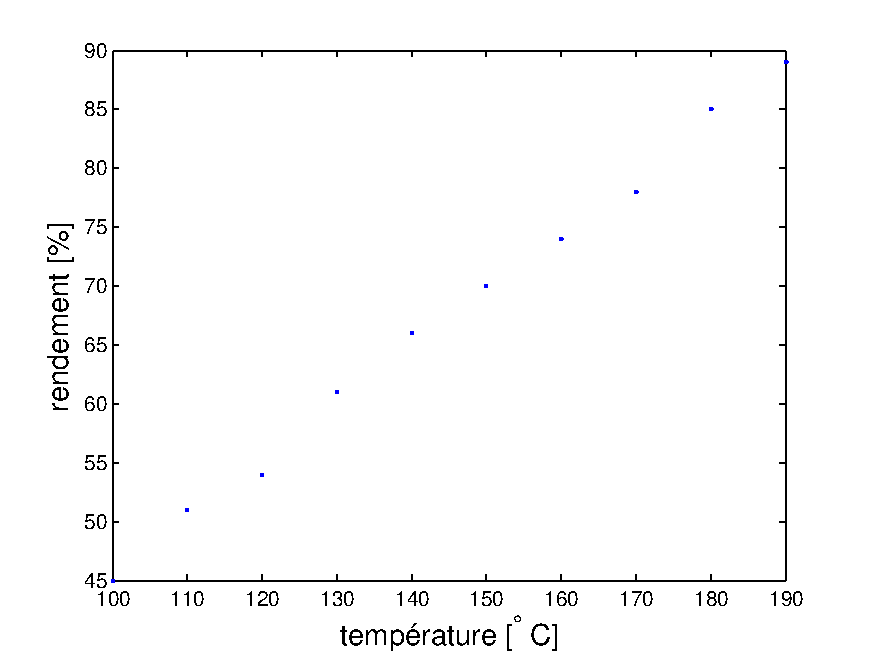
\includegraphics[scale=0.6]{4-Figures/2-scatter_plot_exp.pdf}
\caption{Diagramme de dispersion du rendement en fonction de la température}
\label{fig:scatter_plot_exp}
\end{figure}

On peut constater sur la figure \ref{fig:scatter_plot_exp} qu'il existe une relation forte entre le rendement et la température. Supposons que cette relation est linéaire, il est possible de modéliser ces données à l'aide de l'équation \eqref{eq:reg_lin_simple}. On calcule d'abord
\begin{align*}
 \sum_{i=1}^{10} x_i &=1450, &\hspace{1cm} & \overline{x}= \frac{1}{10} \sum_{i=1}^{10} x_i=145, & \sum_{i=1}^{10} x_i^2 = 218~500,\\
  \sum_{i=1}^{10} y_i&=673, &\hspace{1cm} & \overline{y}= \frac{1}{10} \sum_{i=1}^{10} y_i=67,3, & \sum_{i=1}^{10} Y_ix_i= 101~570.
\end{align*}
On obtient 
\begin{align*}
S_{xx}&=218~500-(1450)^2/10=8250, \cr
S_{xy}&=101~570-1450\times 673/10=3985.
\end{align*}
Et donc
\begin{align*}
\widehat{\beta_1} &= 3985/8250=0,483, \\
\widehat{\beta_0} &= 67,3-0,483\times145=-2,739.
\end{align*}
Le modèle de régression linéaire simple ajusté est $\widehat Y_i=-2,739+0,483x_i$. Ainsi, une augmentation de un degré Celsius de la température du procédé est associée à une augmentation moyenne de $0,483$ point de pourcentage du rendement du produit. Le modèle indique aussi qu'à une température nulle, le rendement attendu est de $-2,739\%$.

La figure~\ref{fig:reg_lin_exp} montre l'ajustement obtenu sous forme d'une droite. Dans ce cas-ci la relation linéaire semble très appropriée pour modéliser la relation entre les variables.

\begin{figure}[h!]
\centering
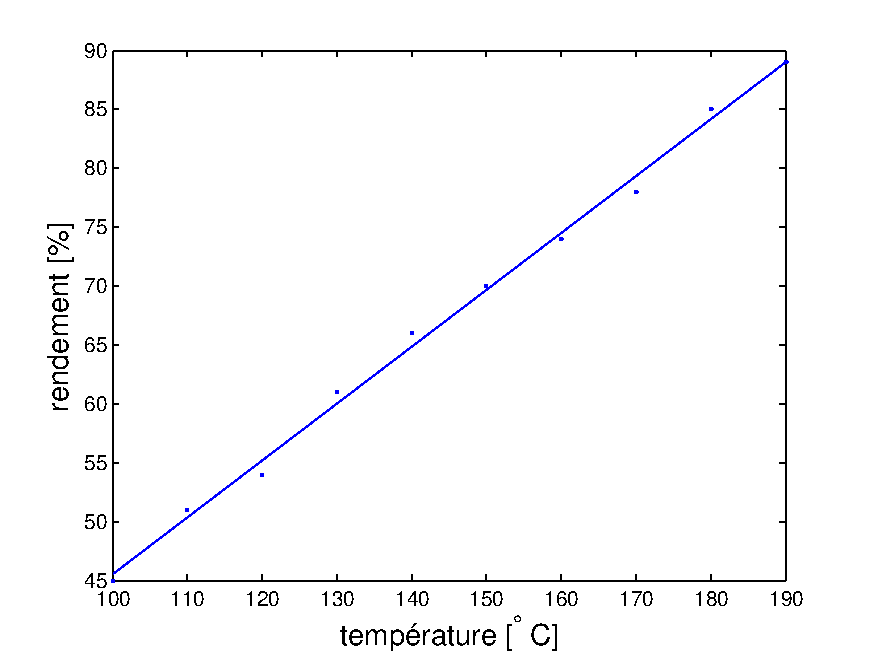
\includegraphics[scale=0.6]{4-Figures/2-reg_lin_exp.pdf}
\caption{Diagramme de dispersion du rendement en fonction de la température avec la droite de régression estimée superposée}
\label{fig:reg_lin_exp}
\end{figure}

On peut également estimer $\sigma^2$ à partir des données. Il faut d'abord calculer la valeur prédite et le résidu pour chacune des observations, comme au Tableau \ref{tab:cal_sigma2_exp}. L'équation~\eqref{sigma2} mène à
$$\widehat{\sigma}^2_{MV}=\frac{1}{10} \{(-0,561)^2+\cdots+(-0,0301)^2\}=\frac{7,224}{10}=0,7224.$$

\begin{table}[h!]
\caption{Tableau résumant $x_i$, $Y_i$, $\hat Y_i$ et $\widehat\varepsilon_i$, $i=1,\dots,10$ pour le calcul de $\widehat\sigma^2_{MV}$ dans l'exemple de la section \ref{exemple-RLS-interpretation}}
\label{tab:cal_sigma2_exp} \centering
\begin{tabular}{c|cccc}
$i$ & $x_i$& $Y_i$ & $\hat Y_i$ & $\widehat\varepsilon_i$ \\ \hline
1 & 100 & 45 & 45,561 &  -0,561 \\
2 & 110  & 51  & 50,391 & 0,609 \\
3 &  120 & 54  & 55,221 & -1,221 \\
4 & 130  & 61 & 60,051 & 0,949\\
5 & 140 & 66  & 64,881  &  1,119 \\
6 & 150  & 70 & 69,711  & 0,289\\
7 &160  & 74 & 74,541 & -0,541\\
8 & 170  & 78 & 79,371 & -1,371\\
9 & 180 & 85 & 84,201 & 0,799\\
10 & 190  & 89 & 89,031 & -0,031
\end{tabular}
\end{table}

% Chapitre 3 - Inférence RLS
\chapter{Inférence pour la RLS} \label{sec:InferenceRLS}
\minitoc \mtcskip \minilof
\section{Inférence sur les paramètres}
\label{sec:InférenceParamètres}

On a montré comment obtenir des estimations pour les différents paramètres du modèle de régression linéaire simple. Généralement, on souhaite également faire de l'inférence sur les vraies valeurs des paramètres $\beta_0$, $\beta_1$ et $\sigma^2$. Pour ce faire, on utilise la distribution des estimateurs.

\subsection{Distribution des estimateurs}
\label{sec:LoisBetas}

\subsubsection{Distribution de $\widehat{\beta}_1$}
\label{sec:LoiDeHatBeta1}

On note d'abord que $\widehat{\beta}_1$ est une combinaison linéaire des $Y_i$. En effet,
\begin{align*} 
\widehat{\beta}_1 &= \frac{\sum\limits_{i=1}^n (x_i-\overline{x})Y_i}{\sum\limits_{i=1}^n (x_i-\overline{x})^2} = \sum_{i=1}^n a_i Y_i, \cr
\intertext{où}
a_i &= \frac{x_i-\overline{x}}{\sum\limits_{i=1}^n(x_i-\overline{x})^2} 
    =  \frac{x_i-\overline{x}}{S_{xx}}.
\end{align*}
Étant donné qu'une combinaison linéaire de variables aléatoires normales suit également une distribution normale, il s'ensuit que $\widehat\beta_1$ est distribué selon une loi normale. Il faut déterminer l'espérance et la variance de $\widehat\beta_1$. Notons d'abord que
 \begin{eqnarray*}
 \sum_{i=1}^n a_i & = & \frac{\sum\limits_{i=1}^n(x_i-\overline{x})} {S_{xx}} = 0, \\
\sum_{i=1}^n a_i x_i & = & \frac{\sum\limits_{i=1}^n(x_i-\overline{x})x_i } {S_{xx}} =\frac{\sum\limits_{i=1}^n(x_i-\overline{x})(x_i-\overline{x})}{S_{xx}}=\frac{S_{xx}}{S_{xx}}=1.
\end{eqnarray*}
Calculons l'espérance  de $\beta_1$,
\begin{eqnarray*}
 \esp\left(\widehat{\beta}_1\right) &=& \sum_{i=1}^n a_i \esp\left(Y_i\right)  \\
 &=& \sum_{i=1}^n a_i \left(\beta_0 + \beta_1 x_i\right)\\
 &=& \beta_0 \sum_{i=1}^n a_i + \beta_1 \sum_{i=1}^n a_i x_i\\
 &=& \beta_1.
\end{eqnarray*}
Ainsi, l'estimateur $\widehat{\beta}_1$ est un estimateur sans biais de $\beta_1$ puisque $\esp\left(\widehat{\beta}_1\right)  - \beta_1 = 0$.
Calculons la variance de $\widehat\beta_1$, 
\begin{eqnarray*}
 \var\left(\widehat\beta_1\right)&=&\var\left(\sum_{i=1}^n a_i Y_i\right)\\
 &=& \sum_{i=1}^n a_i ^2 \, \var\left(Y_i\right)\\
 &=& \sum_{i=1}^n \frac{(x_i-\overline{x})^2}{S_{xx}^2}  \, \var\left(Y_i\right)\\
 &=& \frac{1}{S^2_{xx}} \sum_{i=1}^n (x_i-\overline{x})^2  \, \var\left(Y_i\right)\\
 &=& \frac{S_{xx}}{S_{xx}^2} \sigma^2 \\
 &=& \frac{\sigma^2}{S_{xx}}.
\end{eqnarray*}
Ainsi, la distribution de $\widehat\beta_1$ est
\begin{eqnarray}
\label{distbeta1}
 \widehat{\beta}_1 \sim N\left( \beta_1, \frac{\sigma^2}{S_{xx}} \right).
 \label{loibeta1}
\end{eqnarray}

\begin{remarque}
Seulement certaines hypothèses de la RLS ont été nécessaires pour calculer cette distribution. Lesquelles? Et que nous indique la forme de cette distribution sur l'estimation de la pente dans un modèle de régression linéaire simple?
\end{remarque}


\subsubsection{Distribution de $\widehat\beta_0$}
\label{DistributionBeta0}
L'estimateur $\widehat\beta_0$ peut également s'exprimer comme une combinaison linéaire des $Y_i$,
\begin{eqnarray*}
 \widehat{\beta}_0 &=& \overline{Y} - \widehat{\beta}_1 \overline{x} \\
 &=& \sum_{i=1}^n \frac{Y_i}{n} - \overline{x} \sum_{i=1}^n a_i Y_i \\
 &=& \sum_{i=1}^n \left( \frac{1}{n} - a_i \overline{x}\right) Y_i.
\end{eqnarray*}
Par le même raisonnement que pour $\widehat\beta_1$, on a donc que $\widehat\beta_0$ est distribué selon une loi normale. On peut calculer l'espérance et la variance de $\widehat\beta_1$. Pour l'espérance, on a que
\begin{eqnarray*}
 \esp\left(\widehat{\beta}_0\right) &=& \esp\left(\overline{Y} - \widehat{\beta}_1 \overline{x}\right) \\
 &=& \frac{1}{n}\sum_{i=1}^n \esp\left(Y_i\right) - \overline{x}  \,\esp\left(\widehat{\beta}_1\right)  \\
 &=& \frac{1}{n}\sum_{i=1}^n\left(\beta_0+\beta_1 x_i\right)-\overline{x}\beta_1 \\
 & = & \beta_0+\beta_1 \overline x-\beta_1\overline x \\
 & = & \beta_0.
\end{eqnarray*}
Pour la variance, on a
\begin{eqnarray*}
 \var\left(\widehat{\beta}_0\right) &=& \var\left(\overline{Y} - \widehat{\beta}_1 \overline{x}\right) \\
 &=& \var\left(\frac{1}{n}\sum_{i=1}^n Y_i\right)+ \overline{x}^2 \, \var\left(\widehat{\beta}_1\right)-2\overline x \, \cov\left(\overline Y,\widehat\beta_1\right)  \\
 &=& \frac{\sigma^2}{n}+\overline{x}^2\frac{\sigma^2}{S_{xx}} \\
 & = & \sigma^2\left(\frac{1}{n}+\frac{\overline{x}^2}{S_{xx}}\right).
\end{eqnarray*}
Pour obtenir l'expression finale pour cette variance, il faut démontrer que $\cov[\overline Y,\widehat\beta_1]=~0$, ce qui est laissé en exercice. 
On obtient ainsi la loi pour $\widehat\beta_0$,
\begin{eqnarray}
\label{distbeta0}
 \widehat{\beta}_0 \sim \N\left\{\beta_0, \left(\frac{1}{n}+\frac{\overline{x}^2}{S_{xx}}\right)\sigma^2\right\}.
\label{loibeta0}
\end{eqnarray}

\begin{exemple}
Calculons la variance de $\widehat\beta_0$ et $\widehat\beta_1$ de l'exemple de la section \ref{exemple-RLS-interpretation}. On doit pour ce faire connaître la valeur de la variance des termes d'erreur. Supposons ici que $\sigma^2=1$. On sait déjà que $n=10,\overline x=145$ et $S_{xx}=8250$. Par conséquent on a
\begin{align*}
    \var[\widehat\beta_0] &= \left( \frac{1}{10}+\frac{145^2}{8250} \right)(1)=2,648, \cr
    \var[\widehat\beta_1] &= \frac{1^2}{8250}=1,212\times 10^{-4}.
\end{align*}
\end{exemple}


\subsection{Intervalles de confiance pour $\beta_0$ et $\beta_1$}
\label{sec:IntervallesDeConfiance}

On peut utiliser les distributions de $\widehat{\beta}_0$ et $\widehat{\beta}_1$ pour construire des intervalles de confiance pour $\beta_0$ et $\beta_1$. Pour déterminer l'intervalle de confiance pour $\beta_1$, on centre et réduit la variable aléatoire pour obtenir
\begin{equation}
\frac{\widehat{\beta}_1-\beta_1}{\sqrt{\sigma^2/S_{xx}}}\sim \N(0,1).
\label{disbeta0std}
\end{equation}
%équations \eqref{distbeta0} et \eqref{distbeta1})
\vspace{-0.05 in}
Si $\sigma^2$ était connue, un intervalle de confiance de niveau $100(1-\alpha)\%$ serait donné par 
$$\left[\widehat{\beta}_1\pm z_{1-\alpha/2} \frac{\sigma}{\sqrt{S_{xx}}} \right].$$ 
Or, $\sigma^2$ n'est généralement pas connue et on doit l'estimer. L'estimateur du maximum de vraisemblance de cette quantité est 
$$ \widehat{\sigma}_{MV}^2 = \sum_{i=1}^n \frac{\widehat{\varepsilon}_i^2}{n},$$ mais ce dernier est biaisé.
%Montrer que c'est le cas.
On utilisera donc plutôt l'estimateur non biaisé défini par $$\widehat{\sigma}^2=  \frac{1}{n-2} \sum_{i=1}^n \widehat{\varepsilon}_i^2.$$

\vspace{-0.05 in}
Remplacer $\sigma^2$ par $\widehat\sigma^2$ dans le terme de gauche de \eqref{disbeta0std} a toutefois pour conséquence que cette variable aléatoire ne suit plus une loi normale. On peut néanmoins montrer, en utilisant des notions de statistique mathématique, que
\begin{equation}
 \frac{\displaystyle\frac{\widehat{\beta}_1-\beta_1}{\displaystyle\sigma/\sqrt{S_{xx}}}}
 {  \sqrt{\frac{\displaystyle\widehat\sigma^2}{\displaystyle\sigma^2} } } \sim \mathcal{T}_{n-2}.
\label{disbeta0stds}
\end{equation}
On peut alors déduire un intervalle de confiance de niveau $100(1-\alpha)\%$ pour $\beta_1$,
\begin{eqnarray}
\left[\widehat{\beta}_1 \pm t_{n-2; 1-\alpha/2} \left(\frac{\widehat\sigma}{\sqrt{S_{xx}}}\right)\right],
\end{eqnarray}
où $t_{n-2; 1-\alpha/2}$ dénote le $(1-\alpha/2)$-ième quantile d'une loi $\mathcal{T}$ à $(n-2)$ degrés de liberté.\\

 Il est possible de construire de la même manière un intervalle de confiance pour $\beta_0$. On obtient l'intervalle de confiance 
 \begin{eqnarray}
\left[\widehat{\beta}_0\pm t_{n-2; 1-\alpha/2}\; \widehat\sigma\sqrt{{1\over n}+{\overline{x}^2\over S_{xx}}}\right].
\label{ci:beta0}
\end{eqnarray}

\vspace{0.05in}
\begin{remarque}
Pour arriver à \eqref{disbeta0stds}, on note que
\begin{eqnarray*}
 \frac{\frac{\displaystyle\widehat{\beta}_1-\beta_1}{\displaystyle\sigma/\sqrt{S_{xx}}}}{\sqrt{\frac{\displaystyle\sum_{i=1}^n \widehat{\varepsilon}_i^2}{\displaystyle\sigma^2 (n-2)}}}=\frac{U}{\sqrt{V/\nu}},
\end{eqnarray*}
où $U=\left(\widehat{\beta}_1-\beta_1\right) \big/ \left(\sigma/\sqrt{S_{xx}}\right)$ est distribué selon une loi normale centrée réduite et $V= \left(\sum_{i=1}^n \widehat{\varepsilon}_i^2 \right)\big/ \sigma^2$ suit une loi du khi-carré à $\nu=(n-2)$ degrés de liberté, puisque c'est une somme du carré de variables aléatoires normales.
Comme il s'agit d'un rapport entre une variable aléatoire normale centrée réduite et la racine carrée d'une variable khi-carré divisée par son degré de liberté  $(n-2)$, on obtient la distribution d'une loi $\mathcal{T}$ de Student à $(n-2)$ degrés de liberté ($\mathcal{T}_{n-2}$),
\begin{eqnarray*}
 \frac{\frac{\displaystyle\widehat{\beta}_1-\beta_1}{\displaystyle\sigma/\sqrt{S_{xx}}}}{\sqrt{\frac{\displaystyle\sum_{i=1}^n \widehat{\varepsilon}_i^2}{\displaystyle\sigma^2 (n-2)}}} \sim \frac{\N(0,1)}{\sqrt{\chi_{n-2}^2/(n-2)}} \sim \mathcal{T}_{n-2}.
 \end{eqnarray*}
\end{remarque}


\begin{exemple}
\label{exp:int_beta}
Calculons un intervalle de confiance pour $\beta_0$ et $\beta_1$ de l'exemple \ref{exemple-RLS-interpretation}. La plupart des quantités nécessaires ont déjà été calculées. Il ne manque que
$$\widehat\sigma=\sqrt{\frac{1}{10-2} \sum_{i=1}^{10}\widehat\varepsilon_i^2}=\sqrt{\frac{7,224}{8}}=0,950.$$
Si on fixe $\alpha=5\%$, il faut calculer $t_{n-2; 0,975}$. On peut trouver dans une table que ce quantile est  $t_{8;0,975}=2,306$. On obtient alors les intervalles suivants:
$$\left[\widehat{\beta}_0\pm 2,306\times0,950\sqrt{1/10+145^2/8250} \right]=\left[\widehat{\beta}_0\pm 3,566\right]=\left[-6,305;0,827\right],$$
$$\left[\widehat{\beta}_1\pm 2,306\times 0,950/\sqrt{8250}\right]=\left[\widehat{\beta}_1\pm 0,024\right]=[0,459;0,507].$$
\end{exemple}


\subsection{Tests d'hypothèses}

On peut également se baser sur les distributions déterminées à la section \ref{sec:LoisBetas} pour mettre en {\oe}uvre des tests d'hypothèses sur la valeur des coefficients. Considérons le test bilatéral
\begin{align*}
    \mathcal{H}_0&: \; \beta_j = c, \cr
    \mathcal{H}_1&: \; \beta_j \neq c.
\end{align*}
Notons 
\begin{align*}
    \widehat{\mathrm{Var}}\left(\widehat{\beta}_0\right)
    &= \widehat\sigma^2\left({1\over n}+{\overline{x}^2\over S_{xx}}\right), \\
    \widehat{\mathrm{Var}}\left(\widehat{\beta}_1\right)
    &= \frac{\widehat\sigma^2}{S_{xx}}.
\end{align*}
Sous $\mathcal{H}_0$, 
$$\frac{\widehat{\beta}_j - c}{\widehat{\mathrm{Var}}\left(\widehat{\beta}_j\right)} \sim \mathcal{T}_{n-2}.$$
Soit $t_{obs} = \left(\widehat{\beta}_j - c \right) \big/ \widehat{\mathrm{Var}}\left(\widehat{\beta}_j\right)$ la statistique observée du test. La décision du test d'hypothèses au seuil $\alpha$ peut être prise de trois façons.
\begin{enumerate}[label=(\roman*)]
    \item Valeur critique: Soit le quantile théorique $t_{n-2; 1-\alpha/2}$. Si $|t_{obs}| > t_{n-2; 1-\alpha/2}$, l'hypothèse nulle $\mathcal{H}_0: \; \beta_j = c$ est rejetée.
    \item Valeur-p: Soit $\alpha^* = \prob(|t_{n-2}|>|t_{\text{obs}}|) = 2 \prob(t_{n-2}>|t_{\text{obs}}|)$ la valeur-p. Si $\alpha^* < \alpha$,  l'hypothèse nulle $\mathcal{H}_0: \; \beta_j = c$ est rejetée.
    \item Intervalle de confiance: Si la valeur $c$ n'est pas comprise dans l'intervalle de confiance pour $\beta_j$ de niveau $1-\alpha$, l'hypothèse nulle $\mathcal{H}_0: \; \beta_j = c$ est rejetée.
\end{enumerate}
Il est aussi possible de faire des test unilatéraux. Pour le test
\begin{align*}
    \mathcal{H}_0&: \; \beta_j = c, \cr
    \mathcal{H}_1&: \; \beta_j < c,
\end{align*}
les règles de décisions sont
\begin{enumerate}[label=(\roman*)]
    \item Valeur critique: Si $t_{obs} < - t_{n-2; 1-\alpha}$, l'hypothèse nulle $\mathcal{H}_0: \; \beta_j = c$ est rejetée.
    \item Valeur-p: Si $\alpha^* = \prob(t_{n-2}<t_{\text{obs}}) < \alpha$,  l'hypothèse nulle $\mathcal{H}_0: \; \beta_j = c$ est rejetée.
\end{enumerate}
Pour le test
\begin{align*}
    \mathcal{H}_0&: \; \beta_j = c, \cr
    \mathcal{H}_1&: \; \beta_j > c,
\end{align*}
les règles de décisions sont
\begin{enumerate}[label=(\roman*)]
    \item Valeur critique: Si $t_{obs} > t_{n-2; 1-\alpha}$, l'hypothèse nulle $\mathcal{H}_0: \; \beta_j = c$ est rejetée.
    \item Valeur-p: Si $\alpha^* = \prob(t_{n-2}>t_{\text{obs}}) < \alpha$,  l'hypothèse nulle $\mathcal{H}_0: \; \beta_j = c$ est rejetée.
\end{enumerate}

Un cas particulier, souvent d'intérêt, est le test bilatéral avec $c=0$. Pour la pente, ceci correspond aux hypothèses
$\mathcal{H}_0: \beta_1 = 0$, $\mathcal{H}_1: \beta_1 \neq 0$. Si l'hypothèse nulle de ce test est rejetée, le lien linéaire entre $Y$ et $x$ n'est pas significatif et le modèle se réduit à $Y_i = \beta_0 + \varepsilon_i$. Pour l'ordonnée à l'origine, on a $\mathcal{H}_0: \beta_0 = 0$, $\mathcal{H}_1: \beta_0 \neq 0$. Si l'hypothèse nulle de ce test est rejetée, l'ordonnée à l'origine n'est pas significativement différente de 0 et le modèle se réduit à $Y_i = \beta_1 x_i + \varepsilon_i$.


\begin{exemple}
Toujours avec les données de la section \ref{exemple-RLS-interpretation}, on a
$$ t_{obs} = \frac{\widehat{\beta}_1}{\widehat\sigma/\sqrt{S_{xx}}} = \frac{0,483}{0,950/\sqrt{8250}} = 46,17. $$
Un logiciel nous permet d'obtenir $5.35 \times 10^{-11}$ comme valeur de $p$ correspondante. On rejette donc l'hypothèse d'une pente nulle au seuil $\alpha = 0,05$. Notez qu'on aurait pu arriver à la même conclusion simplement à l'aide de l'intervalle de confiance construit à l'exemple \ref{exp:int_beta}. En effet, l'intervalle de confiance à 95\% pour $\beta_1$ ne contient pas la valeur $0$, ce qui permet de rejeter l'hypothèse que $\beta_1 = 0$ au seuil $\alpha = 0,05$.
\end{exemple}


\section{Prévision}
\label{sec:PrévisionRLS}

On a déjà défini $\widehat{Y}_i = \widehat{\beta}_0 + \widehat{\beta}_1 x_i$, la prévision du modèle en $x_i$. Avant de définir un intervalle de confiance, deux intérêts doivent être distingués:
\begin{enumerate}
\item[(i)] l'estimation de $\esp[Y|x=x_0]$, la valeur moyenne de $Y$ pour une valeur $x=x_0$
de la variable explicative.
\item[(ii)] l'estimation de ${Y}_0^*$, soit la valeur d'une observation/r\'ealisation de $Y$ lorsque la variable explicative prend la valeur $x_0$. 
\end{enumerate}
Dans le premier cas, on souhaite estimer la valeur de la droite en $x_0$, alors que dans le deuxième cas, on s'intéresse à une réalisation de la variable réponse, qui n'est pas nécessairement sur la droite. L'intervalle de confiance sera plus grand dans le deuxième cas, pour tenir compte de la variabilité additionnelle causée par la fluctuation aléatoire autour de la droite.

\subsection{Prévision de la valeur moyenne $\esp[Y|x=x_0]$}

Soit $\esp[Y|x=x_0]$, la valeur moyenne de $Y$ lorsque $x=x_0$. Cette quantité est estimée par $\widehat{Y}_0 = \widehat{\beta}_0 + \widehat{\beta}_1 x_0$.
On utilise le fait que $Y_i \sim \N(\beta_0+\beta_1x_i,\sigma^2)$ pour déterminer la distribution de $\widehat{Y}_0$.
On exprime d'abord $\widehat{Y}_0$ sous la forme d'une combinaison linéaire des $Y_i$,
\begin{align*}
 \widehat{Y}_0 &= \widehat{\beta}_0 + \widehat{\beta}_1 x_0 \\
 &=\sum_{i=1}^n \left(\frac{1}{n} - a_i \overline{x}\right) Y_i + \left(\sum_{i=1}^n a_i Y_i\right) x_0 \\
 &= \sum_{i=1}^n \left(\frac{1}{n} - a_i \overline{x} + a_i x_0\right) Y_i\\
 &= \sum_{i=1}^n c_i Y_i,
 \intertext{où}
 c_i &= \frac{1}{n} - a_i \overline{x} + a_i x_0.
\end{align*}
On peut montrer que $\sum_{i=1}^n c_i = 1$, que $\sum_{i=1}^n c_i x_i = x_0$ et que $\sum_{i=1}^n c_i^2 = 1/n + (\overline{x}-x_0)^2 \big/ S_{xx}$.
On peut ensuite en déduire que
\begin{eqnarray}
 \esp\left(\widehat{Y}_0\right) &=& \sum_{i=1}^n c_i \esp\left(Y_i\right)= \sum_{i=1}^n c_i (\beta_0 + \beta_1 x_i) = \beta_0 + \beta_1 x_0, \\
 \label{eq:varyo}
 \var\left(\widehat{Y}_0\right) &=& \sum_{i=1}^n c_i^2 \var\left(Y_i\right) = \left\{ \frac{1}{n} + \frac{(\overline{x}-x_0)^2}{S_{xx}}\right\} \sigma^2.
 \end{eqnarray}
Puisque $\widehat{Y}_0$ est une combinaison linéaire des $Y_i$, qui suivent une loi normale, $\widehat{Y}_0$ suit aussi une loi normale. On a donc
\begin{equation}
\widehat{Y}_0 \sim \N\left\{\beta_0 + \beta_1 x_0, \left( 1/n + \frac{(\overline{x}-x_0)^2}{S_{xx}}\right) \sigma^2 \right\}.
\end{equation}
À partir de ce résultat, il est possible de calculer un intervalle de confiance autour de la valeur moyenne de $Y$ en $x=x_0$ en remplaçant $\sigma^2$ par son estimateur $\widehat\sigma^2$. En utilisant le même raisonnement qu'à la section \ref{sec:IntervallesDeConfiance}, on obtient l'intervalle de confiance de niveau $1-\alpha$ pour $\esp[Y|x=x_{0}]$,
\begin{eqnarray}
\left[\left(\widehat{\beta}_0 + \widehat{\beta}_1 x_0\right)\; \pm\; t_{n-2; 1-\alpha/2} \;\widehat\sigma \; \sqrt{\frac{1}{n}+\frac{(\overline x-x_0)^2}{S_{xx}}}\right].
\label{eq:int_conf_val_moy_prev}
\end{eqnarray}

 \subsection{Prévision d'une observation $Y_0^*$ lorsque $x=x_0$}

Il est important de comprendre que l'intervalle de confiance défini à l'équation \eqref{eq:int_conf_val_moy_prev} concerne la moyenne de $Y$ au point $x=x_0$. Pour construire ce qu'on appelle un intervalle de prévision, il faut considérer à la fois la variance liée à l'estimation des paramètres et la variance liée à la variabilité naturelle du phénomène, c'est-à-dire la variance du terme d'erreur $\varepsilon$. Or, l'équation \eqref{eq:varyo} ne tient pas compte de la variance du terme d'erreur $\sigma^2$.

Désignons la prévision de la moyenne de $Y$ en  $x_0$ par $\widehat{Y}_0 = \widehat{\beta}_0 + \widehat{\beta}_1 x_0$ et la prévision d'une observation individuelle par $\widehat{Y}_0^* = \widehat{\beta}_0 + \widehat{\beta}_1 x_0 + \varepsilon$. L'espérance de $\widehat{Y}_0$ et celle de $\widehat{Y}_0^*$ sont égales parce que l'espérance des termes d'erreur est nulle. Ce n'est pas le cas des variances.
On a que
\begin{eqnarray}
 \var\left(\widehat{Y}_0^*\right) &=& \var\left(\widehat{Y}_0\right) + \var \left(\varepsilon\right) \nonumber\\
 &=&\left\{ \frac{1}{n} + \frac{(\overline{x}-x_0)^2}{S_{xx}}\right\} \sigma^2 + \sigma^2 \nonumber\\
 &=& \left\{1+\frac{1}{n} + \frac{(\overline{x}-x_0)^2}{S_{xx}} \right\} \sigma^2.
 \label{eq:varyo*}
\end{eqnarray}
Le méthode de calcul de l'intervalle de prévision de niveau $1-\alpha$ pour ${Y}_0^*$ est similaire à celle de l'intervalle de confiance pour  $\esp[Y|x=x_0]$. On obtient donc
\begin{eqnarray}
\left[\left(\widehat{\beta}_0 + \widehat{\beta}_1 x_0\right)\; \pm\; t_{n-2; 1-\alpha/2} \; \widehat\sigma \; \sqrt{1+\frac{1}{n}+\frac{(\overline x-x_0)^2}{S_{xx}}} \right].
\label{eq:int_prev}
\end{eqnarray}


En analysant les expressions \eqref{eq:varyo} et \eqref{eq:varyo*}, nous constatons que les variances diminuent lorsque $n$ augmente ou que $S_{xx}$ augmente. Cela signifie que plus la taille de l'échantillon est grande et/ou plus il y a de la variabilité dans les valeurs de la variable indépendante, plus les estimations seront précises. Au contraire, plus le point $x_0$ pour lequel une prévision est requise est éloigné du centre  de la variable explicative $(\overline x)$, plus la prévision sera imprécise.
Il est important de prendre ces remarques en considération lors de la planification des expériences.


\begin{remarque}
L'intervalle de prévision pour $Y_0^*$ sera toujours plus large que l'intervalle de confiance pour $\esp[Y|x=x_0]$. Pour cette raison, il peut arriver dans la pratique qu'un client préfère présenter l'intervalle de confiance plutôt que l'intervalle de prévision. Il est important de bien comprendre et de bien expliquer la distinction entre les deux intervalles pour éviter une mauvaise interprétation des résultats.
\end{remarque}


\begin{exemple}
On désire calculer un intervalle de confiance au niveau 95 $\%$ pour le rendement moyen du produit ($\esp[Y|x=x_0]$) lorsque la température de fonctionnement est de 150 $^{\circ}\mathrm{C}$ et pour le rendement d'un produit spécifique (${Y}_0^*$) lorsque la température est de 150 $^{\circ}\mathrm{C}$.
Dans les deux cas, la prévision est $\widehat{Y}_0 = \widehat\beta_0+ \widehat\beta_1\times150 =-2,739+0,483\times 150=69,711 \%$.

La plupart des quantités nécessaires au calcul des deux intervalles ont été déjà calculées auparavant. On tire de la section \ref{exemple-RLS-interpretation}  que $\overline x=145, S_{xx}=8250$ et de l'exemple \ref{exp:int_beta} que $\widehat\sigma=0,950$ et que $t_{8; 0,975}=2,306$. Il nous reste seulement à calculer $(x_0-\overline x)^2=(150-145)^2=25$.
En utilisant l'équation \eqref{eq:int_conf_val_moy_prev}, on obtient l'intervalle de confiance du rendement moyen :
$$\left[69,711\pm 2,306\times 0,950\times\sqrt{1/10+25/8250}\right]=\left[69,711 \pm 0,703\right]=[69,008;70,414].$$
L'intervalle de prévision du rendement d'un produit quelconque, appelé également intervalle de prévision, se calcule à l'aide de l'équation~\eqref{eq:int_prev}: 
 $$\left[69,711\pm 2,306\times 0,950\times\sqrt{1+1/10+25/8250}\right]=[69,711\pm 2,301]=[67,410;72,012].$$
Comme mentionné, l'intervalle de prévision est plus large que l'intervalle de confiance pour $\esp[Y|x=150]$.
\end{exemple}


\section{Décomposition de la variance}
\label{sec:AnalyseDeLaVariance}




Une partie de la différence entre les $Y_i$ peut être expliquée par la différence entre les $x_i$, puisque selon le modèle de régression la variable réponse est expliquée en partie par la variable explicative. Il reste une partie de la variabilité des $Y_i$ qui n'est pas expliquée par les différences dans les valeurs de $x_i$. On peut écrire
\begin{align*}
Y_i - \overline{Y} &= \left(\widehat{Y}_i - \overline{Y}\right)  +  \left(Y_i - \widehat{Y}_i\right).
\end{align*}
On a aussi que
\begin{eqnarray*}
  \sum_{i=1}^n \left(Y_i-\overline{Y}\right)^2 & = & \sum_{i=1}^n \left(Y_i - \widehat{Y}_i + \widehat{Y}_i - \overline{Y}\right)^2\\
 &=&  \sum_{i=1}^n \left(Y_i - \widehat{Y}_i\right)^2 + \sum_{i=1}^n\left(\widehat{Y}_i - \overline{Y}\right)^2 + 2\sum_{i=1}^n \left(Y_i-\widehat{Y}_i\right)\left(\widehat{Y}_i-\overline{Y}\right)\\
 &=&  \sum_{i=1}^n \left(Y_i - \widehat{Y}_i\right)^2 + \sum_{i=1}^n\left(\widehat{Y}_i - \overline{Y}\right)^2.
\end{eqnarray*}
Notons
\begin{equation}\label{eq:decompvar}
SC_{tot}=SC_{reg}+SC_{res},
\end{equation}
o\`u
\begin{itemize}
    \item $SC_{tot} =\sum_{i=1}^n(Y_i-\overline{Y})^2$, la somme des carrés totale, quantifie la variabilit\'e des $Y_i$ autour de leur valeur moyenne;
    \item $SC_{reg} =\sum_{i=1}^n(\widehat{Y}_i-\overline{Y})^2$, la somme des carrés de la régression, quantifie la variabilit\'e des prévisions~$\widehat{Y}_i$. Les $\widehat{Y}_i$ ne varient qu'avec les $x_i$, cette somme de carrés est donc la partie de la variabilit\'e des $Y_i$ expliqu\'ee par le fait que toutes les observations n'ont pas la m\^eme valeur de $x_i$;
    \item $SC_{res} =\sum_{i=1}^n(Y_i-\widehat{Y}_i)^2$, la somme des carrés résiduelle, quantifie la variabilit\'e dans les $(Y_i-\widehat{Y}_i)$. Cette variabilit\'e est induite par le fait que la valeur de $Y_i$ n'est pas expliqu\'ee parfaitement par le mod\`ele de r\'egression.
\end{itemize}

\begin{exemple}
\label{exp:ss}
Toujours dans l'exemple du rendement d'un produit en fonction de la température de fonctionnement du procédé, on peut calculer 
\begin{align*}
SC_{tot} &= \sum_{i=1}^n(Y_i-\overline{Y})^2 = 1931,2, \\
SC_{res} &= \sum_{i=1}^n(Y_i-\widehat{Y}_i)^2 = (n-2)*\widehat\sigma^2 = 7,224, \\
SC_{reg} &= \sum_{i=1}^n(\widehat{Y}_i-\overline{Y})^2 = 1924,876.
\end{align*}
On vérifie alors que $SC_{tot} = SC_{reg} + SC_{res}$. On note que la température \`a elle seule ne peut pas expliquer en totalit\'e le fait que toutes les expériences ne possèdent pas le m\^eme rendement.
\end{exemple}

\subsection{Coefficient de détermination}
\label{sec:R2}


La décomposition de la variance permet de quantifier la qualité du modèle de régression linéaire à l'aide du coefficient de détermination,
\begin{equation}
R^2 =\frac{SC_{reg}} {SC_{tot}}.
\end{equation}
Notons que $0 \leq R^2 \leq 1$. Le coefficient de détermination s'interprète comme la proportion de la variance des $Y_i$ expliquée par le modèle. Lorsque $R^2=0$, le mod\`ele n'explique absolument pas la variabilité des $Y_i$. Quand $R^2=1$, tous les points sont alignés sur la droite de r\'egression, c'est-à-dire que l'ajustement du mod\`ele est parfait et que la valeur de $Y_i$ est une fonction exacte de $x_i$. Ainsi, une valeur élevée du $R^2$ indique que le modèle est bon.  Le seuil à partir duquel on considère que le $R^2$ est élevé est très variable et assez subjectif. Il dépend notamment des objectifs de la régression et du domaine d'application.

Le coefficient de détermination correspond au carré de la corrélation entre les valeurs observées et les valeurs prédites
 \[R^2 = \frac{SC_{reg}} {SC_{tot}} = \corr^2 (Y, \widehat{Y})=\left(\frac{\sum_{i=1}^n (Y_i - \overline{Y})(\widehat{Y}_i - \overline{Y})}{\sqrt{\sum_{i=1}^n (Y_i - \overline{Y})^2\sum_{i=1}^n(\widehat{Y}_i - \overline{Y})^2}}\right)^2.
\]


\begin{exemple}
Dans notre exemple,
$$R^2 = \frac{1924,876}{1931,1} = 0,9967,$$
ce qui indique que la température prédit presque parfaitement le rendement de l'expérience. Des valeurs aussi grandes sont plutôt rares en pratique.
\end{exemple}


% Chapitre 4 - Notions pour statistique multivariée
\chapter{Notions pour la statistique multivariée} \label{sec:NotionsMultivarie}
\minitoc \mtcskip \minilof
\section{Notions d'algèbre linéaire}

\subsection{Définitions et opérations sur les matrices}


\begin{defn}
Une \textbf{matrice} réelle $m\times n$ est un tableau ordonné de nombres réels arrangés en $m$ lignes et $n$ colonnes. On appelle ce tableau matrice de dimension $m \times n$. 
Une matrice $\boldA$ et ses éléments $a_{ij}$, $i = 1, \dots, m$ et $j=1, \dots, n$, peuvent s'écrire
$$
\boldA=\left[ \begin{array}{ccccc}
a_{11} & \cdots & a_{1j} & \cdots & a_{1n} \\
\vdots &         & \vdots &           & \vdots \\
a_{i1} &  \cdots       &  a_{ij} & \cdots & a_{in} \\
\vdots &         & \vdots &           & \vdots \\
a_{m1} &  \cdots & a_{mj}& \cdots & a_{mn}
\end{array}
\right].
$$
\end{defn}

\begin{defn}
Soit $\boldA$ une matrice de dimension $m\times n$ quelconque, alors la \textbf{matrice transposée} de $\boldA$, notée $\boldA^\top$ ou $\boldA'$, est de dimension $n\times m$ et comprend les éléments $\alpha_{ji}=a_{ij},\;\;i=1,\ldots,m; \; j=1,\ldots,n.$
\end{defn}

\begin{defn}
    Une matrice carrée (de dimension $n\times n$) $\boldA$ est \textbf{symétrique} si ses éléments sont tels que
    $$ a_{ij} = a_{ji}$$
    pour $i, j = 1, \dots, n$. Une matrice symétrique est égale à sa transposée, $\boldA = \boldA^\top$.
\end{defn}

\begin{defn}
    Soit une matrice $\boldA$ carrée de dimension $n\times n$. La \textbf{matrice inverse} de $\boldA$, notée $\boldA^{-1}$ est la matrice qui satisfait
    $$ \boldA \boldA^{-1} = \boldA^{-1}\boldA = \bold{I}_n,$$
    où $\bold{I}_n$ est la matrice identité de dimension $n$.
\end{defn}

\begin{defn}
    Soit une matrice $\boldA$ carrée de dimension $n\times n$. La matrice $\boldA$ est \textbf{idempotente} si la multiplication par elle-même ne la modifie pas,  
     $\boldA \boldA = \boldA.$
\end{defn}

\begin{defn}
La \textbf{somme matricielle} $\bold{C}=\boldA+\bold B$ de deux matrices $\boldA$ ($m\times n$) et $\bold B$ ($m\times n$) est la matrice $C$ (de même dimension que $\boldA$ et $\bold B$) dont les éléments sont
$$c_{ij}=a_{ij}+b_{ij}\qquad\;\;i=1,\ldots,m; \; j=1,\ldots,n.$$
\end{defn}

\begin{defn}
Le produit du scalaire $k, k\in\R$, et de la matrice $\boldA$ de dimension $m\times n$ est la matrice $\bold C$ de dimension $m\times n$, $\bold{C}=k\boldA$, dont les éléments sont
$$c_{ij}=k a_{ij}\;\;i=1,\ldots,m; \; j=1,\ldots,n.$$
\end{defn}

\begin{defn}
Soient $\boldA$ et $\bold B$ deux matrices de dimensions respectives $m\times r$ et $r\times n$. Le \textbf{produit matriciel} $\bold{C}=\bold A\bold B$ correspond à la matrice $\bold C$ de dimension $m\times n$ dont les éléments sont
$$c_{ij}=\sum_{k=1}^r a_{ik}b_{kj}, \quad i=1,\ldots,m; \; j=1,\ldots,n.$$
Il est à noter que le produit matriciel n'est défini que si le nombre de colonnes de $\boldA$ est égal au nombre de lignes de $\bold B$. L'élément $c_{ij}$ correspond au produit scalaire euclidien du i$^\text{ème}$ vecteur ligne de $\boldA$ par le j$^\text{ème}$ vecteur colonne de $\bold B$.
\end{defn}



\subsection{Propriétés du calcul matriciel}
\label{sec:prop_calc_mat}

En supposant des matrices compatibles pour les opérations en question, on a que

\begin{enumerate}[label=(\roman*)]
\item Commutativité de la somme : $\boldA + \bold B  =  \bold B + \bold A$
\item Associativité de la somme : $(\bold A+\bold B)+\bold C  =  \bold A+ (\bold B+\bold C)$
\item Associativité du produit:  $(\bold A\bold B)\bold C=\bold A(\bold B\bold C)$
\item Divers types de distributivité :
\begin{align*}
  \bold A(\bold B+\bold C)&=\bold A\bold B+\bold A\bold C \\
(\bold A+\bold B)\bold C&=\bold A\bold C+\bold B\bold C \\
k(\bold A+\bold B)&=k\bold A+k\bold B \\
(k_1+k_2)\bold A&=k_1\bold A+k_2\bold A 
\end{align*}

\item Divers types d'associativité : 
\begin{align*}
    k_1(k_2\bold C)&=k_1k_2\bold C \\
    k(\bold A\bold  B)&=(k\bold A) \bold B=\bold A(k\bold B)
\end{align*}
\end{enumerate}


\subsection{Propriétés de la transposition et de l'inversion}
\label{sec:prop_transp}
\begin{enumerate}[label=(\roman*)]
\item $(\bold A+\bold B)^\top=\bold A^\top+\bold B^\top$
\item $(k\bold A)^\top=k\bold A^\top$
\item $(\bold A\bold B)^\top=\bold B^\top \bold A^\top$
\item $(\bold A^\top)^\top=\bold A$
\item $(\bold A^{-1})^{-1}=\bold A$
\item $(\bold A^\top)^{-1}=\bold (\bold A^{-1})^\top$
\item $(\bold A\bold B)^{-1}=\bold B^{-1} \bold A^{-1}$
\end{enumerate}


\subsection{Projection orthogonale}

Soit $\bold V$ un sous-espace vectoriel de $\mathbb{R}^n$ et une matrice $\bold X$ dont les colonnes forment une base de $\bold V$. La \textbf{matrice de projection orthogonale} sur l'espace engendré par les colonnes de $\bold X$ est 
$$ \bold P_{\bold X} = \boX \left( \boX^\top \boX\right)^{-1} \boX^\top. $$
Cette matrice de projection est idempotente et symétrique. Ainsi, $\bold P_{\boX} = \bold P_{\boX}^\top = \bold P_{\boX} \bold P_{\boX}$.

Soit un vecteur $\bold y \in \mathbb{R}^n$. Sa projection sur $\bold V$ est obtenue le multipliant à la matrice de projection, soit $\bold P_{\boX} \bold y$.

\subsection{Dériver une fonction d'un vecteur}
\label{sec:Deriver}

Soit une fonction scalaire $f: \mathbb{R}^n \rightarrow \mathbb{R}$ et un vecteur $\boldx = \left( x_1, \dots, x_n\right)^\top$. Pour dériver $f(\boldx)$ par rapport à $\boldx$, il faut appliquer la dérivée partielle à $f(\boldx)$ par rapport à chaque composante du vecteur $\boldx$. Ainsi,
\begin{align*}
\frac{\partial f(\boldx)}{ \partial \boldx} =
    \begin{pmatrix}
       \displaystyle \frac{\partial f(\boldx)}{\partial x_1} \\[4mm]
       \displaystyle \frac{\partial f(\boldx)}{\partial x_2} \\[4mm]
       \displaystyle \vdots\\[4mm]
       \displaystyle \frac{\partial f(\boldx)}{\partial x_n} 
    \end{pmatrix}.
\end{align*}

\begin{exemple}
    Soit un vecteur $\boldx = \left( x_1, \dots, x_n\right)^\top$, un vecteur $\boldu = \left(u_1, \dots, u_n\right)^\top$ et une matrice symétrique $\boldA$ de dimension $n\times n$.

    \begin{enumerate}[label=(\roman*)]
        \item Calculons $\partial \boldx^\top \boldu \big/ \partial \boldx$. On a
        \begin{align*}
        \boldx^\top \boldu &=
         \begin{pmatrix}
             x_1 & \cdots & x_n
         \end{pmatrix}
         \begin{pmatrix}
             u_1 \\
             \vdots \\
             u_n
         \end{pmatrix}
         =
         x_1 u_1 + \dots x_n u_n
         \intertext{et}
         \frac{\partial \boldx^\top \boldu}{\partial x_1}
         &= u_1, \quad \dots \;, \quad \frac{\partial \boldx^\top \boldu}{\partial x_n} = u_n.
         \intertext{Ainsi,}
         \frac{\partial \boldx^\top \boldu}{\partial \boldx}
         &= 
         \begin{pmatrix}
             \displaystyle \frac{\partial \boldx^\top \boldu}{\partial x_1} \\[4mm]
             \displaystyle\vdots \\[4mm]
             \displaystyle\frac{\partial \boldx^\top \boldu}{\partial x_n}
         \end{pmatrix}
         = \begin{pmatrix}
             u_1 \\[4mm]
             \vdots \\[4mm]
             u_n
         \end{pmatrix}
         = \boldu.
    \end{align*}

    \item Calculons $\partial \boldx^\top \boldA \boldx \big/ \partial \boldx$. On a
        \begin{align*}
        \boldx^\top \boldA \boldx &=
         \begin{pmatrix}
             x_1 & \cdots & x_n
         \end{pmatrix}
         \begin{pmatrix}
             a_{11} & \cdots & a_{1n} \\[4mm]
             \vdots & \ddots & \vdots \\[4mm]
             a_{n1} & \cdots & a_{nn}
         \end{pmatrix}
         \begin{pmatrix}
             x_1 \\
             \vdots \\
             x_n
         \end{pmatrix}
         =
         \sum_{i=1}^n\sum_{j=1}^n x_i x_j a_{ij}
         \intertext{qui peut s'écrire}
         \boldx^\top \boldA \boldx &=
         \sum_{i=1}^n\sum_{\substack{j=1 \\ i\neq j}}^n x_i x_j a_{ij} + \sum_{i=1}^n x_i^2 a_{ii}.
         \intertext{Alors}
         \frac{\partial  \boldx^\top \boldA \boldx }{\partial x_1}
         &= \sum_{i=2}^n x_i a_{i1} + \sum_{j=2}^n x_j a_{1j} + 2 x_1 a_{11} \\
         &= \sum_{i=1}^n x_i a_{i1} + \sum_{j=1}^n x_j a_{1j} \\
         &= 2\sum_{j=1}^n x_j a_{1j}  \quad\text{puisque $A$ est symétrique.}
         \intertext{Ainsi,}
         \frac{\partial \boldx^\top \boldA \boldx }{\partial \boldx}
         &= 
         \begin{pmatrix}
             \displaystyle \frac{\partial \boldx^\top \boldA \boldx }{\partial x_1} \\[4mm]
             \displaystyle\vdots \\[4mm]
             \displaystyle\frac{\partial \boldx^\top \boldA \boldx }{\partial x_n}
         \end{pmatrix}
         = 2 \begin{pmatrix}
             \sum\limits_{j=1}^n x_j a_{1j} \\[4mm]
             \vdots \\[4mm]
             \sum\limits_{j=1}^n x_j a_{nj}
         \end{pmatrix}
         = 2 \boldA \boldx.
    \end{align*}
    \end{enumerate}
\end{exemple}




\section{Espérance et variance de variables aléatoires}

 Soit $\boX=\left(X_1, X_2, \dots, X_n\right)^\top$, un vecteur de
$n$ variables al\'eatoires et $\bo{A}$ et $\bo{B}$, des matrices de constantes. L'espérance de $\boX$ est
\begin{align*}
\esp\left(\boX\right)&=
\begin{pmatrix}
    \esp(X_1)\\[4mm]
    \esp(X_2)\\[4mm]
    \vdots \\[4mm] 
    \esp(X_n)
\end{pmatrix}
\intertext{et la variance de $\boX$ est}
\var\left(\boX\right)&=
\begin{pmatrix}
    \var(X_1) & \cov(X_1,X_2) & \cdots & \cov(X_1,X_n) \\[4mm]
\cov(X_2,X_1) & \var(X_2) & \cdots & \cov(X_2,X_n) \\[4mm]
\vdots & \vdots & \ddots & \vdots \\[4mm]
\cov(X_n,X_1) & \cov(X_n,X_2) & \cdots & \var(X_n)
\end{pmatrix}.
\end{align*}
Les propriétés de l'espérance et de la variance sous forme matricielle sont
\begin{enumerate}[label=(\roman*)]
    \item $\esp\left(\bo{A}\boX+\bo{B}\right)
    =\bo{A}\esp\left(\boX\right)+\bo{B} $
    \item $\var\left(\bo{A}\boX\right) 
    =  \bo{A}\var\left(\boX\right)\bo{A}'$
    \item $\var\left(\bo{A}\boX+\bo{B}\right) 
    =  \bo{A}\var\left(\boX\right)\bo{A}'.$
\end{enumerate} 



%%%%%%%%%%


\section{La loi normale multivariée}
\label{LaLoiNormaleMultivariée}

Dans le cas d'une variable aléatoire $Z$ distribuée selon une loi normale centrée réduite, $Z\sim\N(0,1)$, la densité de $Z$ s'écrit 
\begin{eqnarray*}
 f_Z(z) = \frac{1}{\sqrt{2\pi}} \exp\left( \frac{-z^2}{2}\right).
\end{eqnarray*}
Une variable aléatoire $X$ de distribution normale avec une moyenne $\mu$ et une variance $\sigma^2$ peut s'écrire $X=\sigma Z+\mu$. On dit dans ce cas que $X \sim \N (\mu,\sigma^2)$. La densité de cette variable $X$ s'écrit
\begin{eqnarray*}
	f_X(x) =  \frac{1}{\sqrt{2\pi} \sigma} \exp\left\{-\frac{1}{2} \left(\frac{x- \mu}{\sigma}\right)^2\right\}.
\end{eqnarray*}

On considère maintenant la généralisation pour $n\geq 1$.  Posons $\bo{Z}=\left( Z_1, \dots, Z_n \right)^\top$, un vecteur de variables aléatoires indépendantes et identiquement distribuées suivant chacune une loi  $\N(0,1)$. On a que la densité conjointe des $Z_i$ peut  s'écrire comme
\begin{eqnarray}
f(\bo Z) = f(Z_1, ..., Z_n) &=& \prod_{i=1}^p f(Z_i) \nonumber\\
&=&  \left(\frac{1}{\sqrt{2\pi}}\right)^n \exp\left(-\sum_{i=1}^n \frac{z_i^2}{2}\right)\nonumber\\
 &=& \left(\frac{1}{\sqrt{2\pi}}\right)^n \exp\left(-\frac{1}{2} \bo{Z}'\bo{Z}\right).
\end{eqnarray}
Cette densité conjointe est celle d'une loi normale multivariée de dimension $n$, dont le vecteur des espérances est \textbf{0}, un vecteur $n\times 1$ de zéros, et dont la matrice de variances-covariances est $\I_n$, la matrice identité de dimension ($n \times n$). On peut écrire
\begin{eqnarray*}
\begin{pmatrix}
Z_1 \\[4mm]
Z_2 \\[4mm]
\vdots \\[4mm]
Z_n \\[4mm]    
\end{pmatrix}
\sim \N_n (\textbf{0}, \boI_n) \quad\text{ ou encore, }\bo{Z}\sim \N_n (\textbf{0}, \boI_n).
\end{eqnarray*}
%où $p$ désigne le nombre de variables aléatoires, 

Considérons la transformation de variables $\boX=\bo\mu + \bo\Sigma^{(1/2)}\bo{Z}$, où $\bo\mu$ désigne le vecteur contenant les espérances des $n$ variables et $\bo\Sigma$ dénote la matrice de variances-covariances de $\boX$ (de dimension $n \times n$). La densité conjointe des $X_i$ est alors donnée par
\begin{eqnarray}
f(\bo X) = f(X_1, ..., X_n) 
  &=& \left(\frac{1}{\sqrt{2\pi}}\right)^n \frac{1}{\left|\bo\Sigma\right|^{1/2}} \exp\left\{-\frac{1}{2} (\boX- \bo\mu)' (\bo\Sigma^{-1/2})' \bo\Sigma^{-1/2} (\boX- \bo\mu)\right\}\nonumber\\
 &=& \left(\frac{1}{\sqrt{2\pi}}\right)^n \frac{1}{\left|\bo\Sigma\right|^{1/2}} \exp\left\{-\frac{1}{2} (\boX- \bo\mu)' \bo\Sigma^{-1} (\boX- \bo\mu)\right\}.
\label{normalemulti}
\end{eqnarray}
Cette densité est celle d'une loi normale multivariée de dimension $n$, et on peut écrire
\begin{eqnarray*}
\begin{pmatrix}
X_1 \\[4mm]
X_2 \\[4mm]
\vdots \\[4mm]
X_n \\[4mm]    
\end{pmatrix} \sim \N_n \left(\bo\mu, \bo\Sigma\right) \quad\text{ ou encore, }\bo{X}\sim \N_n \left(\bo\mu, \bo\Sigma\right) .
\end{eqnarray*}


\begin{remarque}
   On a posé $\boX=\bo\mu + \bo\Sigma^{(1/2)}\bo{Z}$. 
On peut déterminer l'espérance et la variance de $\boX$ à partir de celles de $\bo{Z}$.
\begin{eqnarray*}
	\esp[\boX] &=& \esp[\bo{\mu} + \bo\Sigma^{1/2}\bo{Z}]\\
	& =& \esp[\bo\mu]+ \bo\Sigma^{1/2}\esp[\bo{Z}] \\
	&=& \bo\mu,
\end{eqnarray*}
\begin{eqnarray*}
	\var[\boX] &=& \var[\bo\Sigma^{1/2}\bo Z] \\
	& = & (\bo\Sigma^{1/2})' \var[\bo Z] \bo\Sigma^{1/2} \\
	&=& (\bo\Sigma^{1/2})' \boI_p \bo\Sigma^{1/2} \\
	&=& \bo\Sigma.
\end{eqnarray*} 
\end{remarque}

\begin{remarque}
    On pourrait appliquer la transformation inverse et déduire le vecteur des variables aléatoires centrées réduites  comme suit: $$\bo Z =  \bo\Sigma^{(-1/2)} (\boX-\bo\mu).$$
\end{remarque}

Finalement, il est possible de transformer une variable aléatoire normale. Voici un cas particulier d'intérêt pour le cours.

\begin{theorem}
\label{thmNormalChi2}
Si $\boX \sim \N_n(\bo 0,\boI_n)$ et $\bo A$ est une matrice symétrique, alors $\boX^\top\bo A\boX \sim \chi^2_r$ si et seulement si $\bo A$ est idempotente de rang r.
\end{theorem}


% Chapitre 5 - Ajuster RLM
\chapter{Ajuster un modèle de régression linéaire multiple (RLM)} \label{sec:AjusterRLM}
\minitoc \mtcskip \minilof


\section{Le modèle de régression linéaire multiple}
\label{sec:ModèleEtNotation}

Le modèle de régression linéaire multiple constitue une généralisation du modèle de régression linéaire simple permettant d'étudier la relation une variable réponse $Y$ avec $p$ variables explicatives  $x_1, x_2, ..., x_p$. L'équation du modèle de régression linéaire multiple s'exprime de la manière suivante
\begin{align}\label{eq:reg_lin_mult}
	Y_i = \beta_0 + \beta_1 x_{i1} +  \beta_2 x_{i2}+ \ldots + \beta_p x_{ip} + \varepsilon_i, \;\;\;\;\;\; i=1,\ldots,n;\;\;\; j=1,\ldots,p,
\end{align}
où
\begin{itemize}
\item $Y_i$ est une variable aléatoire représentant la réponse de l'unité $i$;
\item $x_{ij}$ est la valeur (connue) de la $j$-ème variable explicative de l'unité $i$;
\item $\beta_0$ et $\beta_j,\, j=1,\dots, p$, sont les paramètres du modèle;
\item $\varepsilon_i$ est une variable aléatoire représentant le terme d'erreur de l'unité $i$.
\end{itemize}
Notons 
\begin{itemize}
\item $n$, le nombre d'observations;
\item $p$, le nombre de variables explicatives;
\item $p'=p+1$, le nombre de paramètres à estimer;
\item $\boY = \begin{pmatrix} Y_1 & \cdots & Y_n \end{pmatrix}^\top$, le vecteur $n \times 1$ contenant les $n$ observations à venir (pas encore observées) de la variable réponse;
\item $\bobeta = \begin{pmatrix} \beta_0 & \beta_1 & \cdots & \beta_p \end{pmatrix}^\top$, le vecteur $p' \times 1$ contenant les $p'$ coefficients de régression;
\item $\boeps = \begin{pmatrix} \varepsilon_1 & \cdots & \varepsilon_n \end{pmatrix}^\top$, le vecteur $n\times 1$ des termes d'erreur;
\item $\boX$, la matrice de design (ou d'incidence) $n \times p'$ contenant les observations des $p$ variables explicatives (incluant une colonne de 1 associée à $\beta_0$),
$$\boX = \begin{pmatrix}
        1 & x_{11} & x_{12} & \cdots & x_{1p}  \\
        1 & x_{21} & x_{22} & \cdots & x_{2p}  \\
        \vdots & \vdots & \vdots & \ddots & \vdots \\
        1 & x_{n1} & x_{n2} & \cdots & x_{np}  
    \end{pmatrix}.$$
\end{itemize}
Le modèle de régression linéaire multiple peut s'écrire à l'aide d'une notation matricielle,
\begin{align}
    \underbrace{\begin{pmatrix}
        Y_1 \\
        Y_2  \\
        \vdots \\
        Y_n
    \end{pmatrix}}_{n\times 1}
    &=
    \underbrace{\begin{pmatrix}
        1 & x_{11} & x_{12} & \cdots & x_{1p}  \\
        1 & x_{21} & x_{22} & \cdots & x_{2p}  \\
        \vdots & \vdots & \vdots & \ddots & \vdots \\
        1 & x_{n1} & x_{n2} & \cdots & x_{np}  
    \end{pmatrix}}_{n \times (p+1)}
    \underbrace{\begin{pmatrix}
        \beta_0 \\
        \beta_1 \\
        \vdots \\
        \beta_p 
    \end{pmatrix}}_{(p+1) \times 1}
    +
    \underbrace{\begin{pmatrix}
        \varepsilon_1 \\
        \varepsilon_2 \\
        \vdots \\
        \varepsilon_n 
    \end{pmatrix}}_{n \times 1}, \nonumber
    \intertext{que l'on écrit}
    \boY &= \boX \bobeta + \boeps.
    \label{eq:reg_lin_mult_mat}
\end{align}


\begin{exemple}\label{RLSRLM1}
Dans le cas de la régression linéaire simple, $p=1$ et on peut écrire
\begin{align*}
    \boY = \underbrace{\begin{pmatrix}
        Y_1 \\
        Y_2  \\
        \vdots \\
        Y_n
    \end{pmatrix}}_{n\times 1}, \quad
    \boX =
    \underbrace{\begin{pmatrix}
        1 & x_{1}   \\
        1 & x_{2}  \\
        \vdots & \vdots \\
        1 & x_{n}  
    \end{pmatrix}}_{n \times 2}, \quad
    \bobeta = \underbrace{\begin{pmatrix}
        \beta_0 \\
        \beta_1 
    \end{pmatrix}}_{2 \times 1}, \quad
    \boeps = \underbrace{\begin{pmatrix}
        \varepsilon_1 \\
        \varepsilon_2 \\
        \vdots \\
        \varepsilon_n 
    \end{pmatrix}}_{n \times 1}, 
\end{align*}
On a alors
\begin{align*}
    \begin{pmatrix}
        Y_1 \\
        Y_2  \\
        \vdots \\
        Y_n
    \end{pmatrix}
    =
    \begin{pmatrix}
        1 & x_{1}   \\
        1 & x_{2}  \\
        \vdots & \vdots \\
        1 & x_{n}  
    \end{pmatrix}
    \begin{pmatrix}
        \beta_0 \\
        \beta_1 
    \end{pmatrix}
    +
    \begin{pmatrix}
        \varepsilon_1 \\
        \varepsilon_2 \\
        \vdots \\
        \varepsilon_n 
    \end{pmatrix}
    =
    \begin{pmatrix}
        \beta_0 + \beta_1 x_1 + \varepsilon_1 \\
        \beta_0 + \beta_1 x_2 + \varepsilon_2 \\
        \vdots \\
        \beta_0 + \beta_1 x_n + \varepsilon_n
    \end{pmatrix}, 
\end{align*}
et le modèle de régression linéaire simple défini à l'équation \eqref{eq:reg_lin_simple} peut s'exprimer 
\begin{equation*}
\boY=\boX\bobeta+\boeps.
\end{equation*}
\end{exemple}

\subsection{Postulats du modèle de RLM}
\label{sec:PostulatsRLM}

Les postulats émis sur le modèle de régression linéaire multiple sont les mêmes que ceux émis sur le modèle de régression linéaire simple. Pour $i, \, j=1, \dots, n$, on a
\begin{enumerate}
  \item[$\mathcal{P}_1$.] La linéarité de la relation entre la variable réponse et les variables explicatives, $\esp[\varepsilon_i]=0$;
 \item[$\mathcal{P}_2$.] L'homoscédasticité (variance constante) des observations de la variable réponse, $\var[\varepsilon_i]=\sigma^2$;
 \item[$\mathcal{P}_3$.] L'indépendance des observations de la variable réponse, $\cov(\varepsilon_i,\varepsilon_j)=0 \mbox{ pour } i \neq j$;
 \item[$\mathcal{P}_4$.] La normalité des termes d'erreur, $\varepsilon_i \sim \N(0,\sigma^2)$.
\end{enumerate}


\subsection{Interprétation des paramètres}
\label{sec:InterpétationRLM}

Dans le modèle de RLM  défini à l'équation~\eqref{eq:reg_lin_mult}, et sous le postulat $\mathcal{P}_1. \; \esp[\varepsilon_i]=0$ pour $i=1, \dots, n$, le coefficient $\beta_0$ représente la valeur moyenne de $Y_i$ lorsque $x_{i1}, \ldots, x_{ip}$ prennent toutes simultanément la valeur 0. Le coefficient $\beta_j$, $j=1, \dots, p$, représente la variation dans la moyenne de $Y_i$ lorsque $x_j$ augmente d'une unité et que la valeur de toutes les autres variables explicatives reste constante.

Dans le modèle de régression linéaire simple, les points $Y$ sont situés autour d'une droite, alors que dans le modèle de régression linéaire multiple, ils sont dispersés autour d'un hyperplan.  Le coefficient $\beta_j$ représente la pente de l'hyperplan dans la direction de la variable explicative $j$. Voir la figure \ref{fig:rlm}.
\begin{figure}[h!]
\centerline{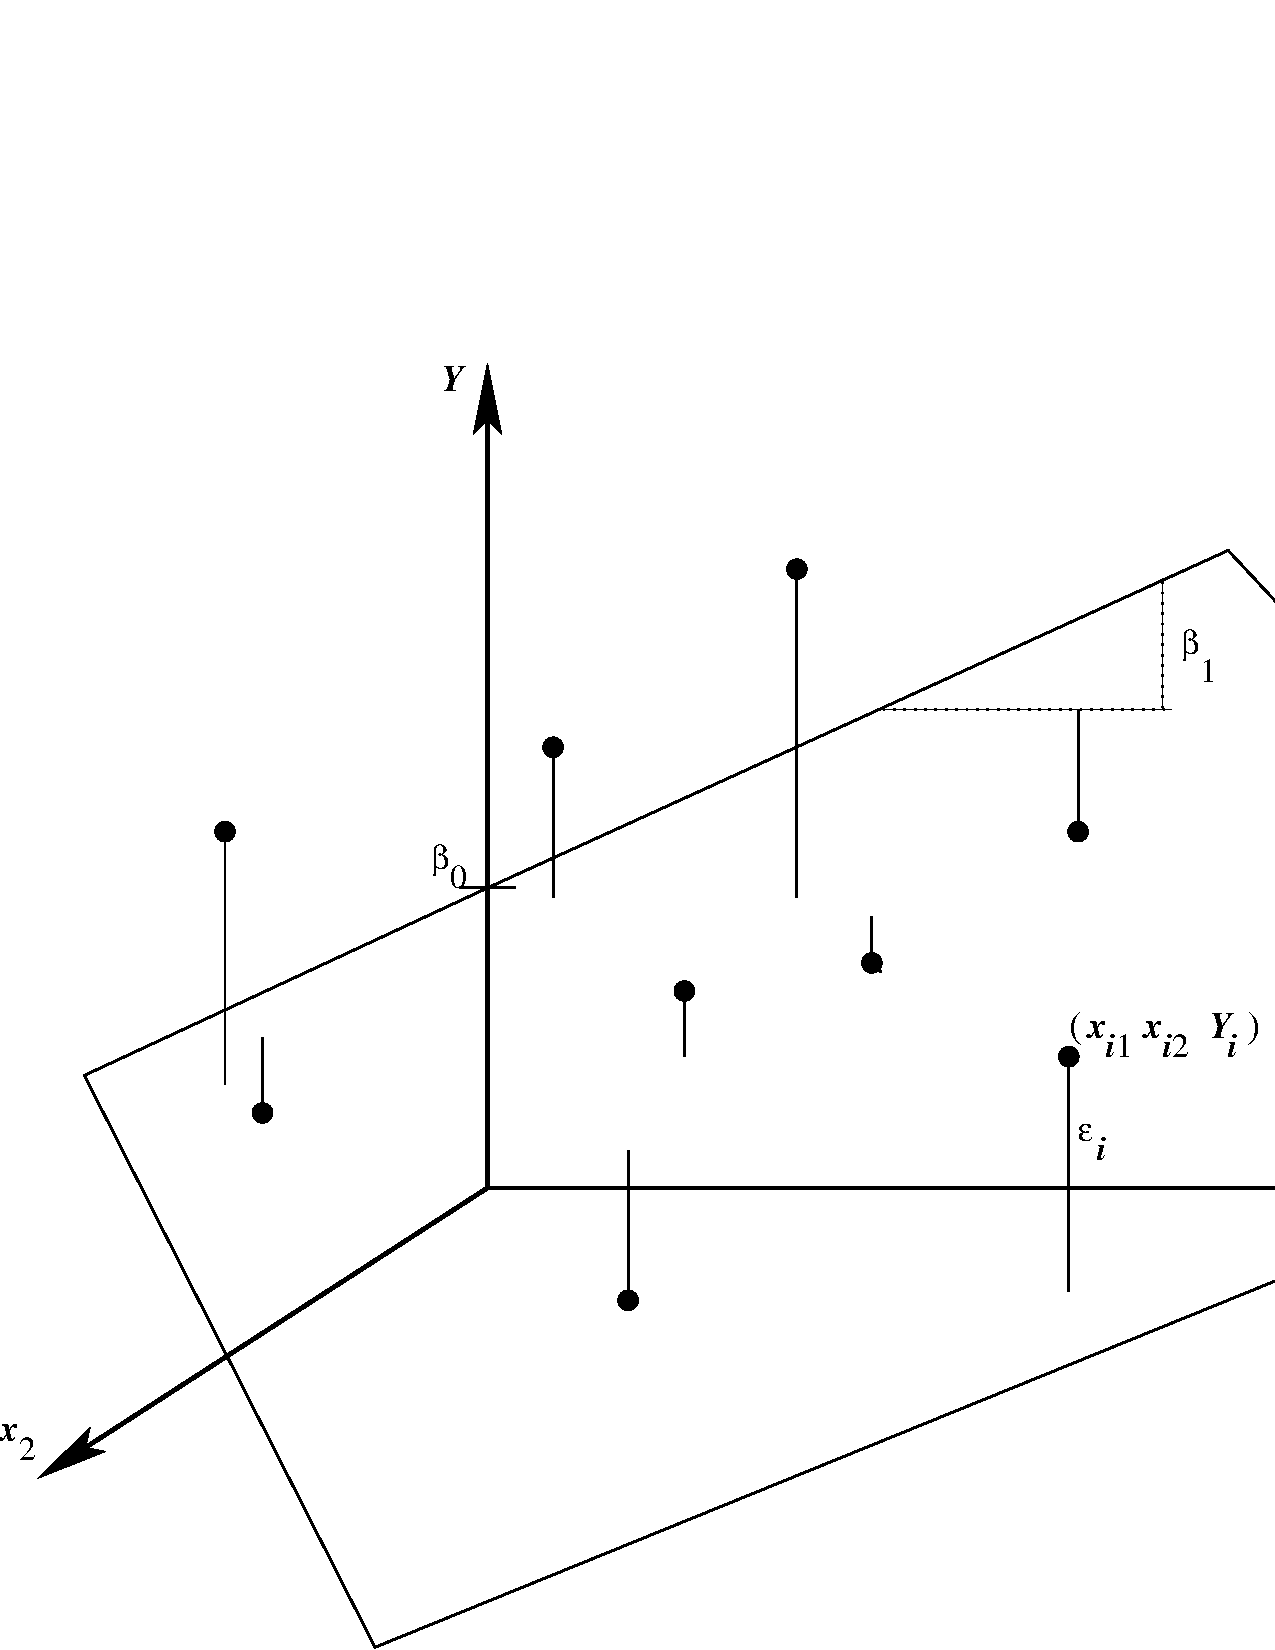
\includegraphics[scale=0.35, trim={0 0 0 5cm}]
{Chap5-AjusterRLM/Figures/reg_mult.pdf}}
\caption{Représentation géométrique du modèle de régression linéaire multiple.}\label{fig:rlm}
\end{figure}



\section{Estimation des coefficients}
\label{sec:EstimationParamètres}

Les coefficients de régression $\beta_0,\, \beta_1, \, \dots, \, \beta_p$ doivent être estimés. Nous présentons dans cette section la méthode des moindres carrés et une approche géométrique. Il est aussi possible d'utiliser la méthode du maximum de vraisemblance pour obtenir des estimateurs des coefficients, ce qui ne sera pas présenté dans le cadre de la RLM.

\subsection{Méthode des moindres carrés}
\label{sec:EstimationRLMMoindresCarrés}

Comme dans le cas de la régression linéaire simple, on adopte à nouveau le principe des moindres carrés de Legendre. On cherche par conséquent le vecteur $\bobeta$ qui minimise la somme des carrés des résidus ($\sum_{i=1} ^n{\widehat{\varepsilon}_i^2}$). Le vecteur des résidus s'exprime
	\[ \boeps = \left({\varepsilon}_1 , \, {\varepsilon}_2, \, ... , \, {\varepsilon}_n\right)^\top = \boY - \boX \bobeta, \]
on a alors
	\[\sum_{i=1}^n {\varepsilon}_i^2= \boeps^\top \boeps= (\boY - \boX \bobeta)^\top (\boY - \boX \bobeta)= f(\bobeta).\]
La fonction $f(\hbobeta)$ s'écrit comme
\begin{eqnarray*}
	f(\bobeta)
    &=& \left[\boY^\top - (\boX \bobeta)^\top\right](\boY - \boX \bobeta) \\
	&=& \boY^\top \boY - \boY^\top \boX \bobeta - (\boX\bobeta)^\top \boY + (\boX\bobeta)^\top (\boX\bobeta) \\
	&=& \boY^\top \boY - 2\bobeta^\top\boX^\top\boY  + \bobeta^\top\boX^\top  \boX\bobeta.
\end{eqnarray*}
Dans la dernière égalité on a que $\boY^\top\boX\bobeta=(\boX\bobeta)^\top\boY=\bobeta^\top\boX^\top\boY$ puisque ces trois quantités sont des scalaires.

Ainsi, pour minimiser $\sum_{i=1} ^n{\widehat{\varepsilon}_i^2}$, il faut dériver $f(\bobeta)$ par rapport à $\bobeta$, puis évaluer la dérivée au point $\hbobeta$ et égaler à 0. En utilisant les notions de la section \ref{sec:Deriver}, on obtient
\[\frac{\partial f(\bobeta)}{ \partial \bobeta} = -2\boX^\top \boY + 2\boX^\top \boX \bobeta.\]
On a ensuite 
\begin{align}
    -2\boX^\top \boY + 2\boX^\top \boX \hbobeta &= 0 \nonumber\\
    \boX^\top \boX \hbobeta  &= \boX^\top \boY \nonumber\\
    \hbobeta  &= \left( \boX^\top \boX \right)^{-1}\boX^\top \boY , \label{eq:est_beta}
\end{align}
si $\boX^\top \boX$ est inversible (de plein rang).
Notons que
\begin{eqnarray*}
	\underbrace{\hbobeta}_{p'\times 1}=\underbrace{(\boX^\top \boX)^{-1}}_{p'\times p'} \underbrace{\boX^\top}_{p'\times n} \underbrace{\boY}_{n\times 1}.
\end{eqnarray*}

\begin{remarque}
La matrice $\boX^\top \boX$ n'est pas  inversible si le nombre d'observations $n$ est inférieur au nombre de paramètres à estimer $p'$, ou si une ligne de cette matrice est une combinaison linéaire des autres. Dans le premier cas, une méthode d'estimation de modèle plus complexe peut être utilisée, comme présenté à la section \ref{sub:lasso}. Dans le second cas, une variable peut être retirée du modèle, voir le chapitre \ref{sec:Multicolinéarité} sur la multicolinéarité.
\end{remarque}

\begin{exemple}
    {\bf Application au cas $p=1$}

    Comme vu dans l'exemple \ref{RLSRLM1}, le modèle de RLS est un cas particulier du modèle de RLM. Vérifions que l'équation (\ref{eq:est_beta}) mène aux estimateurs obtenus au Chapitre \ref{sec:AjusterRLS}.
    En reprenant la notation de l'exemple \ref{RLSRLM1}, on a que 
    \begin{align*}
        \boX^\top \boX
        &=
        \begin{pmatrix}
        1 & 1 & \cdots & 1   \\
        x_1 & x_{2} & \cdots & x_n  
    \end{pmatrix}
        \begin{pmatrix}
        1 & x_{1}   \\
        1 & x_{2}  \\
        \vdots & \vdots \\
        1 & x_{n}  
    \end{pmatrix}
    = \begin{pmatrix}
        n & \sum\limits_{i=1}^n x_i  \\[4mm]
        \sum\limits_{i=1}^n x_i  & \sum\limits_{i=1}^n x_i^2
    \end{pmatrix}
    = 
    \begin{pmatrix}
        n & n \overline{x} \\[4mm]
         n \overline{x}   & \sum\limits_{i=1}^n x_i^2
    \end{pmatrix}
    \end{align*}
   On calcule l'inverse de cette matice $2\times 2$. Le déterminant est 
   $$	\mathrm{det}(\boX^\top\boX) = n \sum_{i=1}^n x_i^2 - n^2\overline{x}^2
	= n \left(\sum_{i=1}^n x_i^2 - \sum_{i=1}^n \overline{x}^2\right)
	= n \sum_{i=1}^n  (x_i^2 - \overline{x}^2)
	= n \sum_{i=1}^n  (x_i - \overline{x})^2
	= n S_{xx}. $$
    Alors
    \begin{align*}
        \left(\boX^\top \boX\right) ^{-1}
        =  \frac{1}{nS_{xx}} \begin{pmatrix}
            \sum\limits_{i=1}^n x_i^2 & -n\overline{x}\\
            -n\overline{x} & n 
        \end{pmatrix}.
    \end{align*}
    Calculons $\hbobeta$,
    \begin{align*}
        \hbobeta
        &= (\boX^\top \boX)^{-1} \boX^\top \boY \\
        &= \frac{1}{nS_{xx}} \begin{pmatrix}
            \sum\limits_{i=1}^n x_i^2 & -n\overline{x}\\
            -n\overline{x} & n 
            \end{pmatrix}
            \begin{pmatrix}
                1 & 1 & \cdots & 1   \\
                x_1 & x_{2} & \cdots & x_n  
            \end{pmatrix}
            \begin{pmatrix}
                Y_1 \\ \vdots \\ Y_n
            \end{pmatrix} \\
        &= \frac{1}{nS_{xx}} \begin{pmatrix}
            \sum\limits_{i=1}^n x_i^2 & -n\overline{x}\\
            -n\overline{x} & n 
            \end{pmatrix}
            \begin{pmatrix}
                \sum\limits_{i=1}^n Y_i \\[4mm]
                \sum\limits_{i=1}^n x_iY_i 
            \end{pmatrix} \\
        &= \frac{1}{nS_{xx}} \begin{pmatrix}
            n\overline{Y}\sum\limits_{i=1}^n x_i^2  - n\overline{x} \sum\limits_{i=1}^n x_i Y_i \\[4mm]
            -n\overline{x}\sum\limits_{i=1}^n Y_i  + n \sum\limits_{i=1}^n x_i Y_i
        \end{pmatrix} \\
        &= \begin{pmatrix}
        \frac{\displaystyle\overline Y\left( \sum\limits_{i=1}^n x_i^2-n\overline x^2\right)-\overline x\left(\sum\limits_{i=1}^n  x_i Y_i-n\overline x\overline Y\right)}{\displaystyle S_{xx}} \\
            \frac{\displaystyle  \sum\limits_{i=1}^n x_i Y_i - n\overline{x} \overline{Y}}{\displaystyle S_{xx}} 
        \end{pmatrix} \\
        &= \begin{pmatrix}
        \frac{\displaystyle \overline{Y}S_{xx} - \overline{x}S_{xy}}{\displaystyle S_{xx}} \\
            \frac{\displaystyle S_{xy}}{\displaystyle S_{xx}}
        \end{pmatrix} 
        = \begin{pmatrix}
        \overline{Y} - \overline{x} \widehat{\beta}_1 \\
            \frac{\displaystyle S_{xy}}{\displaystyle S_{xx}}
        \end{pmatrix}
        = \begin{pmatrix}
            \widehat{\beta}_0 \\\widehat{\beta}_1
        \end{pmatrix}.
    \end{align*}
    On obtient les mêmes résultats qu'en \eqref{eq:beta0} et \eqref{eq:beta1chapeau}.
\end{exemple}


\subsection{Argument géométrique}
\label{sec:ArgumentGéométrique}

Il est possible d'obtenir l'estimateur (\ref{eq:est_beta}) à partir d'une approche géométrique. Le vecteur $\boY$ peut s'écrire comme une combinaison linéaire des colonnes de $\boX$, plus une erreur $\boeps$:
\begin{align*}
\boY &= \boX \bobeta + \boeps \\
    &=   \begin{pmatrix}
        \bf 1 & \bold{x}_{1}  & \cdots & \bold x_{p}  
    \end{pmatrix}
    \begin{pmatrix}
        \beta_0 \\
        \vdots \\
        \beta_p 
    \end{pmatrix}
    +    \boeps \\
    &= \beta_0 {\bf 1} + \beta_1 {\bold x}_{1} + \dots + \beta_p \bold x_{p} + \boeps,
\end{align*}
avec $\bold 1 = (1, \dots, 1)^\top$ $\bold x_j = (x_{1j}, \dots, x_{nj})^\top$.

Soit le sous-espace vectoriel formé par les colonnes de $\boX$. Si $\boX$ est de plein rang (inversible), cet espace aura $p'=p+1$ dimensions. Pour estimer les paramètres du modèle de régression linéaire multiple, on peut projeter $\boY$ dans le sous-espace vectoriel engendré par les colonnes $\boX$. Cette projection orthogonale permet d'obtenir la partie de $\boY$ qui est linéairement expliquées par les colonnes de $\boX$.

Soit $\boH$ la matrice chapeau, c'est-à-dire la matrice de projection orthogonale dans l'espace engendré par les colonnes de $\boX$ (voir la section \ref{sec:MatriceChapeau} pour plus de détails sur cette matrice). 
Le vecteur $\hY$ est le vecteur de valeurs prédites et correspond à la projection orthogonale de $\boY$ sur le sous-espace engendré par les colonnes de $\boX$,
\begin{align*}
    \hY = \boH \boY.    
\end{align*}
Ainsi, $\hY$ s'exprime comme une combinaison linéaire des vecteurs $\bf 1$ et $\bold x_j$, $j=1, \dots, p$.
Le vecteur de résidus $\hboeps$ s'écrit 
$$\hboeps = \boY-\hY = (\boI_n-\boH)\boY.$$ 
Ainsi, le vecteur $\hboeps$ est perpendiculaire au sous-espace engendré par les colonnes de $\boX$, il est une projection de $\boY$ dans le sous-espace perpendiculaire à celui engendré par les colonnes de $\boX$. Toujours en considérant $\boX$ de plein rang, ce sous-espace est de dimension $(n-p')$. La projection orthogonale permet de minimiser la somme des résidus au carré, c'est-à-dire $\hboeps'\hboeps$. L'orthogonalité de $\hY$ et $\hboeps$ revient à dire que $\cov[\hboeps, \hY] = 0$. En effet, des vecteurs orthogonaux sont des vecteurs non corrélés. Dans le cas gaussien, ceci implique de plus que ces vecteurs sont indépendants.
La figure \ref{fig:geometrie} représente géométriquement le cas où $n=3$ $p'=2$. 


\definecolor{bleufonce}{RGB}{30,74,126}
\definecolor{bleuclair}{RGB}{64,120,190}
\definecolor{planbleu}{RGB}{231,239,248}

\begin{figure}
    \centering
    \begin{tikzpicture}[line cap=round,
                    line join=round,
                    >=stealth,
                    scale=1.15]
% Sommets du plan
\coordinate (A) at (0,0);
\coordinate (B) at (5.8,-0.75);
\coordinate (C) at (7.6,1.75);
\coordinate (D) at (1.8,2.5);
% Origine des vecteurs, projection et extrémité de Y
\coordinate (O) at (2.30,0.52);
\coordinate (P) at (4.72,1.02);
\coordinate (Y) at (4.72,3.92);
% Plan vectoriel
\filldraw[fill=planbleu,
        fill opacity=0.6,
        draw=bleufonce,
        line width=1.2pt] (A) -- (B) -- (C) -- (D) -- cycle;
% Vecteur Y
\draw[->, color=bleuclair, line width=1.1pt] (O) -- (Y);
% Projection de Y sur le plan
\draw[->, dotted, color=bleuclair, line width=1.1pt] (O) -- (P);
% Résidu orthogonal
\draw[->, dotted, color=bleuclair, line width=1.1pt] (P) -- (Y);
% Symbole d'angle droit
\coordinate (Q1) at ($(P)!0.18!(O)$);
\coordinate (Q2) at ($(P)!0.16!(Y)$);
\coordinate (Q3) at ($(Q1)+(Q2)-(P)$);
\draw[color=bleuclair, line width=0.9pt] (Q1) -- (Q3) -- (Q2);
% Étiquettes
\node[above left=1pt, font=\large] at ($(O)!0.68!(Y)$) {$\bf{Y}$};
\node[below=5pt, rotate=10, font=\large] at ($(O)!0.68!(P)$)
    {$\widehat{\boY}=\boH\boY$};
\node[right=8pt, font=\large] at ($(P)!0.60!(Y)$)
    {$\widehat{\boeps}=(\boI_n-\boH)\mathbf{Y}$};
\end{tikzpicture}
    \caption{Représentation géométrique de la régression dans le cas où $p=1$ et $n=3$.}
    \label{fig:geometrie}
\end{figure}


Pour obtenir $\hbobeta$ sous cette approche, on peut utiliser le fait que l'on veut écrire $\widehat{\boY} = \boX \hbobeta$ et que $\hY$ est perpendiculaire à $\hboeps$,
\begin{align*}
    \hY^\top \hboeps &= 0 \\
    \left(\boX \hbobeta\right)^\top \hboeps &= 0  \\
     \hbobeta^\top \boX^\top \hboeps &= 0,  \\
 \intertext{ainsi}    
    \boX^\top \hboeps &= 0  \\
    \boX^\top(\boY-\boX\hbobeta) &= 0 \\
    \boX^\top\boY - \boX^\top\boX\hbobeta &= 0 \\
    \boX^\top\boY &= \boX^\top\boX\hbobeta  \\
    \left(\boX^\top\boX\right)^{-1}\boX^\top\boY &= \hbobeta  
\end{align*}
et on retrouve les résultats obtenus avec les moindres carrés, soit l'équation (\ref{eq:est_beta}).






\section{Exemple}

Cet exemple est tiré de \citet[][Exemple 14.1]{Hin_Mon_Gol_Bor:12}.
%\citet{Rag_Ber:01} exposent une analyse consistant à trouver un modèle de prévision des meurtrissures des pommes durant le tri et l'emballage.
Des expériences en laboratoire ont montré que le diamètre des meurtrissures (en mm) peut être expliqué en fonction de la hauteur de chute (en mm) et de la masse volumique des fruits (en g/cm$^3$). Le Tableau \ref{exp_data} présente des données typiques de ce type d'expérience.

Le modèle de régression linéaire multiple s'exprime sous forme matricielle comme
$$
\underbrace{\left(
\begin{array}{c}
3,62  \\
7,27  \\
2,66 \\
1,53 \\
\vdots \\
5,23  \\
\end{array} \right)}_{20\times 1}
 =  \underbrace{\left(\begin{array}{ccc}
            1	&      303,7  & 0,9     \\
            1	&      366,7  & 1,04    \\
            1 &         336,8 & 1,01 \\
            1 &           304,5 & 0,95 \\
            \vdots & \vdots & \vdots   \\
            1	&      351,4  & 0,96
\end{array}\right)}_{20\times 3}
\underbrace{\left(\begin{array}{c}
\beta_0 \\
\beta_1 \\
\beta_2
\end{array} \right)}_{3\times 1}+
\underbrace{\left(\begin{array}{c}
\varepsilon_1 \\
\varepsilon_2 \\
\varepsilon_3 \\
\varepsilon_4 \\
\vdots \\
\varepsilon_{20}
 \end{array}
 \right)}_{20\times 1}
 $$
Selon l'équation (\ref{eq:est_beta}), on sait que $\hbobeta=(\boX^\top\boX)^{-1}\boX^\top \boY$.
La matrice $\boX^\top\boX$ est
\begin{eqnarray*}
\boX^\top\boX & = & \left(
\begin{array}{cccc}
1 & 1 & \cdots & 1 \\
303,7 & 366,7 & \cdots & 351,4 \\
0,90 & 1,04 & \cdots & 0,96
\end{array}
\right)
\left(
\begin{array}{ccc}
1 & 303,7 & 0,90 \\
1 & 366,7 & 1,04 \\
\vdots & \vdots & \vdots \\
1 & 351,4 & 0,96
\end{array}
\right) \\
& = & \left(
\begin{array}{ccc}
20 & 7767,8 & 19,33 \\
7767,8 & 3201646 & 7791,878 \\
19,93 & 7791,878 & 19,9077
\end{array}
\right).
\end{eqnarray*}
Le vecteur $\boX^\top\boY$ s'exprime comme
\begin{eqnarray*}
\left(
\begin{array}{cccc}
1 & 1 & \cdots & 1 \\
303,7 & 366,7 & \cdots & 351,4 \\
0,90 & 1,04 & \cdots & 0,96
\end{array}
\right)
\left(
\begin{array}{c}
3,62 \\
7,27 \\
\vdots \\
5,23
\end{array}
\right)
=
\left(
\begin{array}{r}
120,79 \\
51129,17 \\
122,70
\end{array}
\right).
\end{eqnarray*}
On en déduit donc que
\begin{eqnarray*}
\left(
\begin{array}{c}
\hat\beta_0 \\
\hat\beta_1 \\
\hat\beta_2
\end{array}
\right)
& = &
\left(
\begin{array}{ccc}
20 & 7767,8 & 19,33 \\
7767,8 & 3201646 & 7791,878 \\
19,93 & 7791,878 & 19,9077
\end{array}
\right)^{-1}
\left(
\begin{array}{r}
120,79 \\
51129,17 \\
122,70
\end{array}
\right) \\
& = &
\left(
\begin{array}{rrr}
24,63666 & 0,005321 & -26,74679 \\
0,005321 & 0,0000077 & -0,008353 \\
-26,74679 & -0,008353 & 30,096389
\end{array}
\right)
\left(
\begin{array}{r}
120,79 \\
51129,17 \\
122,70
\end{array}
\right) \\
& = &
\left(
\begin{array}{r}
-33,8310 \\
0,0134 \\
34,8900
\end{array}
\right).
\end{eqnarray*}
Par conséquent, le modèle de régression ajusté s'écrit 
$$\hat Y=-33,831+0,0134x_1+34,890x_2.$$
L'espérance du diamètre moyen des meurtrissures d'une pêche de masse volumique nulle lancée d'une hauteur nulle (très hypothétique comme valeur!) est de $-33,831$ mm. L'augmentation d'un mm de la hauteur de la chute est associée à une augmentation attendue de 0,0134 mm du diamètre moyen des meurtrissures, pour une masse volumique constante. De même, l'augmentation d'un $g/cm^3$ de la masse volumique d'une pêche est associée à une augmentation attendue de $34,890$ mm du diamètre moyen des meurtrissures, pour une hauteur de chute constante.


\begin{table}[htb!]
\caption{Données pour l'exemple des meurtrissures de pêches}
\label{exp_data}
\begin{tabular}{|c|c|c|c|} \hline
numéro &  diamètre des meurtrissures  & hauteur de chute  & masse volumique  \\
 & [mm] & [mm] & [g/cm$^3$] \\
        & $Y_i$        & $x_{i1}$      &  $x_{i2}$ \\ \hline
 1   &   3,62  &   303,7  & 0,90      \\
 2   &   7,27  &   366,7  & 1,04     \\
 3   &   2,66  &  336,8   & 1,01     \\
 4   &   1,53  &  304,5   & 0,95      \\
 5   &   4,91  &  346,8   & 0,98      \\
 6   &   10,36 &   600,0    & 1,04       \\
 7   &   5,26  &   369,0    & 0,96       \\
 8   &   6,09  &   418,0    & 1,00           \\
 9   &   6,57  &   269,0    & 1,01        \\
 10  &   4,24  &   323,0    & 0,94         \\
 11  &   8,04  &   562,2  & 1,01          \\
 12  &   3,46  &   284,2  & 0,97           \\
 13  &   8,50   &   558,6  & 1,03           \\
 14  &   9,34  &   415,0    & 1,01            \\
 15  &   5,55  &   349,5  & 1,04            \\
 16  &   8,11  &   462,8  & 1,02            \\
 17  &   7,32  &   333,1  & 1,05            \\
 18  &   12,58 &   502,1  & 1,10            \\
 19  &   0,15  &   311,4  & 0,91            \\
 20  &   5,23  &   351,4  & 0,96            \\   \hline
\end{tabular}

\end{table}



% Chapitre 6 - Inférence RLM
\chapter{Inférence pour la RLM} 
\label{sec:InferenceRLM}
\minitoc \mtcskip \minilof

\section{Distribution de l'estimateur}

Déterminons la distribution des estimateurs pour faire de l'inférence sur les paramètres.  Pour trouver la loi des estimateurs, on doit faire l'hypothèse que le vecteur des termes d'erreurs $\boeps$ est distribuée selon une loi normale multivariée de dimension égale au nombre d'observations $n$. 
On peut écrire cette hypothèse sous la forme
$$\boeps=\left(\varepsilon_1,\varepsilon_2,...,\varepsilon_n\right)^\top \sim \N_n(\textbf{0}, \sigma^2\bold{I}_n)$$
où  $\bold{I}_n$ dénote la matrice identité de dimension $n\times n$.
On a donc que
\begin{eqnarray*}
	\boY \sim \N_n (\boX\bobeta, \sigma^2 \bold{I}_n).
\end{eqnarray*}

Afin de déterminer l'espérance et la variance de $\widehat{\bobeta}$, on suit la même approche que pour la régression linéaire simple et on exprime $\widehat{\bobeta}$ comme une combinaison linéaire des $Y_i$.
On a vu que
\begin{eqnarray*}
	\widehat{\bobeta}=(\boX^\top\boX)^{-1}\boX^\top\boY.
\end{eqnarray*}
On a donc que $\widehat{\bobeta} \sim \N_{p'}\left(\esp[\widehat{\bobeta}],\var[\widehat{\bobeta}]\right)$ car une combinaison linéaire de variables aléatoires normales est également normalement distribuée. Il reste à calculer $\esp[\widehat{\bobeta}]$ et $\var[\widehat{\bobeta}]$ afin de déterminer la loi complètement.
On peut d'abord montrer que l'estimateur est non biaisé:
\begin{eqnarray*}
	\esp\left[\widehat{\bobeta}\right]&=&\esp\left[(\boX^\top\boX)^{-1}\boX^\top\boY\right] \\
	&=& (\boX^\top\boX)^{-1}\boX^\top \esp\left[\boY\right]\\
	&=& (\boX^\top\boX)^{-1}\boX^\top \boX\bobeta\\
	&=& \bobeta
\end{eqnarray*}
On calcule ensuite la variance:
\begin{eqnarray*}
	\var\left[\widehat{\bobeta}\right]&=& \var\left[(\boX^\top\boX)^{-1}\boX^\top\boY\right]\\
	&=& (\boX^\top\boX)^{-1}\boX^\top \var\left[\boY\right] \left\{(\boX^\top\boX)^{-1}\boX^\top\right\}^\top\\
	&=& (\boX^\top\boX)^{-1}\boX^\top \sigma^2\bold{I}_n \left\{(\boX^\top\boX)^{-1}\boX^\top\right\}^\top\\
	&=& \sigma^2 (\boX^\top\boX)^{-1} \boX^\top \boX(\boX^\top\boX)^{-1}\\
	&=& \sigma^2 (\boX^\top\boX)^{-1}
\end{eqnarray*}
Ainsi,
\begin{eqnarray}
	\widehat{\bobeta} \sim \N_{p'}\{\bobeta,\sigma^2 (\boX^\top\boX)^{-1}\}.
	\label{loibeta}
\end{eqnarray}

\begin{exemple}
{\bf{Application au cas $p=1$}}\label{sec:VarCovDesEstimateur}

On a déjà vu que dans le cas où $p=1$,
\begin{equation}
\label{invxtx}
(\boX^\top \boX) ^{-1}
 =
\frac{1}{nS_{xx}}
\begin{pmatrix}
   \displaystyle \sum_{i=1}^n x_i^2 & -n\overline{x}\\[4mm]
-n\overline{x} & n \\
\end{pmatrix}.
\end{equation}
À partir de \eqref{loibeta} et \eqref{invxtx}, on peut calculer les variances et la covariance de $\widehat{\beta}_0$ et de $\widehat{\beta}_1$,
\begin{eqnarray*}
	\var\left(\widehat{\beta}_1\right)&=&\frac{\sigma^2 n}{n S_{xx}} = \frac{\sigma^2}{S_{xx}}\\[4mm]
	\var\left(\widehat{\beta}_0\right)&=&\frac{\displaystyle\sigma^2 \sum_{i=1}^n x_i^2}{n S_{xx}} = \frac{S_{xx} + n\overline{x}^2}{nS_{xx}} \sigma^2\\[4mm]
	\cov\left(\widehat{\beta}_1,\widehat{\beta}_0\right)&=& \frac{-n\overline{x} \sigma^2}{n S_{xx}}= \frac{-\overline{x} \sigma^2}{S_{xx}}
\end{eqnarray*}
On obtient les quantités déjà connues. Remarquez que la covariance entre $\widehat{\beta}_0$ et $\widehat{\beta}_1$ est de signe contraire de $\overline{x}$ et que cette covariance est nulle si $\overline{x}=0$.
\end{exemple}




\section{Matrice chapeau et implications}
\label{sec:MatriceChapeau}

On a introduit la matrice chapeau, à la section \ref{sec:ArgumentGéométrique}. Dans cette section, on explore plus en détails la matrice chapeau, et on obtient quelques résultats utiles pour l'inférence à partir de ses propriétés.

\subsection{La matrice chapeau}
\label{sec:LaMatriceChapeau}

La matrice chapeau $\boH$ («hat matrix») tire son nom du fait qu'elle permet de transformer $\boY$ en $\hY$ ("Y chapeau"). Selon l'équation \eqref{eq:reg_lin_mult_mat}, la régression linéaire multiple s'exprime sous format matriciel comme $\boY = \boX\bobeta + \boeps$.
L'estimateur de $\bobeta$ peut s'écrire selon l'équation \eqref{eq:est_beta} comme $\widehat{\bobeta} = (\boX^\top\boX)^{-1}\boX^\top\boY$. On peut écrire
\begin{eqnarray*}
	\hY& =& \boX\widehat{\bobeta} \\
    &= & \boX(\boX^\top\boX)^{-1}\boX^\top\boY\\
    &=& \boH\boY
\end{eqnarray*}
La matrice chapeau correspond donc à la matrice $\boH=\boX(\boX^\top\boX)^{-1}\boX^\top$.
Il est également possible d'exprimer les résidus en fonction de la matrice chapeau,
	\[\hboeps=\boY-\hY = \left[\bold{I}_n- \boX(\boX^\top\boX)^{-1}\boX^\top\right]\boY = (\bold{I}_n-\boH)\boY.
\]

% a continuer ici
La matrice chapeau peut être vue comme une matrice de transformation. Il s'agit d'un opérateur linéaire, de même que ($\bold{I}_n-\boH$). Ces deux opérateurs possèdent plusieurs propriétés intéressantes, à savoir :

\begin{enumerate}
   \item $\boH^\top=\boH$ (symétrie);
	\item $\boH\boH=\boH$ (idempotence);
	\item $\boH\boX=\boX$;
     \item $(\bold{I}_n-\boH)^\top=(\bold{I}_n-\boH)$ (symétrie);
	\item $(\bold{I}_n-\boH)(\bold{I}_n-\boH)=(\bold{I}_n-\boH)$ (idempotence);
	\item $(\bold{I}_n-\boH)\boX=0$.
\end{enumerate}
De plus, tous les éléments de la matrice ont une interprétation précise et utile pour étudier la robustesse d'un modèle de RLM. Nous y reviendrons à la section \ref{sec:DonneesInfluentes}.


\subsection{Distribution de $\widehat{\vect{Y}}$ et $\widehat{\vect{\varepsilon}}$}
\label{sec:distYhatEps}

Les propriétés de la matrice chapeau permettent de calculer la variance de $\hY$ et $\hboeps$.
En effet,
\begin{eqnarray*}
	\var\left(\hY\right) = \var\left(\boH\boY\right)=\boH\var\left(\boY\right)\boH^\top= \boH\boH^\top \sigma^2 = \boH \sigma^2
\end{eqnarray*}
et
\begin{eqnarray*}
	\var\left(\hboeps\right)=\var\left((\bold{I}_n-\boH)\boY\right)= (\bold{I}_n-\boH)\sigma^2.
\end{eqnarray*}

On a donc que les lois de $\hY$ et $\hboeps$ sont respectivement
\begin{eqnarray*}
	\hY \sim \N_n(\boX\bobeta, \sigma^2\boH)
\end{eqnarray*}
\begin{eqnarray}
	\hboeps \sim \N_n(\bold{0}, \sigma^2(\bold{I}_n-\boH)).
	\label{distepsilon}
\end{eqnarray}


\subsection{Estimation de $\sigma^2$}
\label{sec:RLM-sigma}

La méthode du maximum de vraisemblance permet de trouver un estimateur pour $\sigma^2$, mais celui-ci est biaisé. On utilise plutôt l'estimateur suivant:
\begin{eqnarray}
	\widehat{\sigma}^2=\frac{\hboeps^\top\hboeps}{n-p'},
	\label{estimationSigma}
\end{eqnarray}
où $p'=p+1$.
Montrons que l'estimateur donné en (\ref{estimationSigma}) est sans biais pour $\sigma^2$, c'est-à-dire, montrons que
$$ E \left( \frac{\hboeps^\top\hboeps}{n-p'} \right) = \sigma^2. $$
Commençons par étudier $\hboeps$ et $\hboeps^\top\hboeps$.
Par  le résultat~(\ref{distepsilon}), $\hboeps \sim \N_n\left(\bold{0}, \sigma^2(\bold{I}_n-\boH)\right)$, et on peut écrire
$$ \frac{\hboeps}{\sigma} \sim \N_n\left(\bold{0}, (\bold{I}_n-\boH)\right).$$
Soit un vecteur $\bo Z \sim \N_n(\bo 0, \bold{I}_n)$. On a que $(\bold{I}_n - \boH)\bo Z \sim \N_n\left(\bold{0}, (\bold{I}_n-\boH)\right)$. Ainsi, on peut écrire 
$$ \frac{\hboeps}{\sigma} = (\bold{I}_n - \boH)\bo Z \sim \N_n\left(\bold{0}, (\bold{I}_n-\boH)\right).$$
Cette forme nous permet d'utiliser le théorème \ref{thmNormalChi2} du Chapitre \ref{sec:NotionsMultivarie}. On a 
\begin{itemize}
\item[$\bullet$] $\bo Z \sim \N_n(\bo 0,\bold{I}_n)$,
\item[$\bullet$] $(\bold{I}_n-\boH)$ une matrice symétrique,
\item[$\bullet$] $(\bold{I}_n-\boH)$ une matrice idempotente idempotente.
\end{itemize}
Avec le Théorème \ref{thmNormalChi2},
$$ \bo Z^\top(\bold{I}_n-\boH) \bo Z \sim \chi^2_r,$$
avec $r$ = rang$(\bold{I}_n-\boH) = n-p'$. 
Or,
\begin{align*}
\bo Z^\top(\bold{I}_n-\boH) \bo Z &= \bo Z^\top(\bold{I}_n-\boH)^\top(\bold{I}_n-\boH) \bo Z \\
&= ((\bold{I}_n-\boH)\bo Z)^\top (\bold{I}_n-\boH) \bo Z \\
&= \frac{\hboeps^\top}{\sigma} \frac{\hboeps}{\sigma} \\
&= \frac{\hboeps^\top\hboeps}{\sigma^2}.
\end{align*}
Ainsi,
$$ \frac{\hboeps^\top\hboeps}{\sigma^2} \sim \chi^2_{n-p'}.$$


On peut finalement montrer que l'estimateur donné en (\ref{estimationSigma}) est sans biais pour $\sigma^2$,
\begin{align*}
E \left( \frac{\hboeps^\top\hboeps}{\sigma^2} \right) &= n-p' \\
E \left( \hboeps^\top\hboeps \right) &= \sigma^2 (n-p') \\
E \left( \frac{\hboeps^\top\hboeps}{n-p'} \right) &= \sigma^2.
\end{align*}


\section{Intervalle de confiance et test d'hypothèse pour un coefficient}
\label{sec:infbetaRLM}

On a utilisé le postulat de normalité $\boeps \sim \N_n(0,\sigma^2\bold{I}_n)$, pour montrer que $\widehat{\bobeta} \sim \N_{p'}\left(\bobeta,\sigma^2 (\boX^\top\boX)^{-1}\right)$. Si on s'intéresse à un $\beta_j$ en particulier, on a alors que
\begin{eqnarray*}
	\frac{\widehat{\beta}_j-\beta_j}{\sigma \sqrt{v_{j+1,j=1}}} \sim \N(0,1),
\end{eqnarray*}
où $v_{j+1,j=1}$ est l'élément $(j+1,j+1)$ de la matrice $(\boX^\top\boX)^{-1}$, pour $j=0, \dots, p$.

On a montré que $\widehat{\sigma}^2 = \hboeps^\top\hboeps / (n-p')$ est un estimateur sans biais de $\sigma^2$. Par conséquent,
\begin{eqnarray}
	\frac{\displaystyle\frac{\widehat{\beta}_j-\beta_j}{\sigma \sqrt{v_{j+1,j+1}}}}{\displaystyle\sqrt{\frac{\hboeps^\top\hboeps}{\sigma^2(n-p')}}} \sim \frac{\N(0,1)}{\sqrt{\chi^2_{n-p'}/(n-p')}} \sim \mathcal{T}_{n-p'},
	\label{loistudentbeta}
\end{eqnarray}
où $\mathcal{T}_{n-p'}$ note la loi de Student à $n-p'$ degrés de liberté. On peut alors utiliser \eqref{loistudentbeta} pour construire un intervalle de confiance pour $\beta_j$ ou pour effectuer des tests d'hypothèses.
L'intervalle de confiance de niveau $(1-\alpha)$ pour $\beta_j$ s'exprime comme
\begin{eqnarray}
\left[ \widehat\beta_j\pm t_{n-p';1-\alpha/2}\sqrt{\widehat\sigma^2 v_{j+1,j+1}} \right]
\label{intconf_beta}
\end{eqnarray}

\begin{exemple}
Construisons un intervalle de confiance à 95 $\%$ pour le paramètre $\beta_1$ de l'exemple de la section \ref{exp_data}. Nous avons déjà calculé que $\widehat\beta_1=0,01314$. L'élément diagonal de la matrice $(\boX^\top\boX)^{-1}$ correspondant à $\beta_1$ est $v_{22}=0,0000077$. L'estimation non biaisée de $\sigma^2$ est $\widehat\sigma^2=2,247$. Le quantile à 97,5 $\%$ d'une loi $\mathcal{T}$ de Student à $n-p'=20-3=17$ degrés de liberté est égal à 2,110.  On obtient donc selon \eqref{intconf_beta} l'intervalle de confiance suivant :
\begin{align*}
\left[ \widehat\beta_1\pm t_{n-p'; 1-\alpha/2}\sqrt{\widehat\sigma^2 v_{22}} \right] &=\left[0,01314\pm2,110\sqrt{2,247\times 0,0000077}\right]\\
&=[0,00436;0,0219]
\end{align*}
On note que l'intervalle n'inclut pas la valeur 0. On peut donc rejeter l'hypothèse nulle $H_0: \beta_1=0$  et conclure que la hauteur de la chute est significativement associée au diamètre moyen des meurtrissures, en tenant compte de la présence des autres variables explicatives dans le modèle.
\end{exemple}


\section{Prévision}
\label{sec:PrévisionRLM}


Quand on veut faire une prévision, on s'intéresse à une combinaison linéaire des coefficients. Considérons donc le problème général d'estimer une combinaison linéaire de $\bobeta$:
\begin{equation}
\sum_{i=0}^p a_i \beta_i = \bo a^\top\bobeta,
	\hspace{1cm} \mbox{o\`u} \quad \bo a^\top=\left(a_0\ a_1 \ ... \ a_p\right).
\label{eq:abeta}
\end{equation}
On peut utiliser $\bo a^\top\widehat{\bobeta}$ pour estimer $\bo a^\top\bobeta$, puisque
\begin{equation}
\bo a^\top\widehat{\bobeta} \sim \N(\bo a^\top\bobeta, \quad \sigma^2\bo a^\top(\boX^\top\boX)^{-1}\bo a).
\label{eq:distabeta}
\end{equation}


\subsection{Inférence pour  $\vect{a}^\top\vect{\beta}$ }
\label{sec:TestsDHypothèsetheta}


On peut utiliser (\ref{eq:distabeta}) pour faire de l'inférence sur une combinaison linéaire des coefficients.
Si on connaissait $\sigma^2$, on pourrait construire des intervalles de confiance et des tests d'hypothèses pour $\bo a^\top\bobeta$ à partir de
\begin{eqnarray}
	\frac{\bo a^\top\widehat{\bobeta}-\bo a^\top\bobeta}{\displaystyle\sqrt{\sigma^2\bo a^\top(\boX^\top\boX)^{-1}\bo a}} \sim \N(0,1).
\end{eqnarray}
Toutefois, comme on ne connaît pas $\sigma^2$, on l'estime par $\widehat{\sigma}^2=\hboeps^\top\hboeps / (n-p')$  et on a que
\begin{eqnarray}
		\frac{\bo a^\top\widehat{\bobeta}-\bo a^\top\bobeta}{\displaystyle\sqrt{\widehat{\sigma}^2\bo a^\top(\boX^\top\boX)^{-1}\bo a}} \sim \mathcal{T}_{n-p'}.
		\label{distprevision}
\end{eqnarray}
On peut  utiliser ce résultat pour construire un intervalle de confiance ou pour faire un test pour~$\bo a^\top\bobeta$.

\begin{remarque}
Il y a plusieurs circonstances dans lesquelles on voudrait faire de l'inférence sur une combinaison linéaire des coefficients. On pourrait se demander si une variable a un effet aussi grand qu'une autre (on s'intéresse alors à $\beta_i - \beta_j$), ou si une variable a un effet deux fois plus grand qu'une autre ($\beta_i - 2\beta_j$), par exemple. Dans les prochaines sections, le résultat (\ref{distprevision}) est appliqué au cas de la prévision pour de nouvelles observations.
\end{remarque}


\subsection{Inférence sur $\esp\left(Y|\vect{x}\right)$}
\label{sec:previsionRLM1}

On désire dans ce cas estimer la valeur moyenne de la variable réponse pour une combinaison de valeurs $\bold{x}^{*\top}=(1, x_1^*,\ldots,x_{p}^*)$ spécifiées des variables explicatives. On veut donc estimer
$\esp\left(Y|\bold{x}^*\right)=\esp\left(\bold{x}^{*\top}\bobeta+\bm{\varepsilon}\right)=\bold{x}^{*\top}\bobeta$.
Cela revient à estimer une combinaison linéaire de $\bobeta$ et il suffit de  remplacer $\bold{x}^{*\top}$ par $\bo a^\top$ dans la section précédente afin d'obtenir un intervalle de confiance au niveau $100(1-\alpha)\%$ pour $\esp\left(Y|\bold{x}^*\right)$.
Celui-ci est donné par
\begin{equation}\label{ci:EY}
\left[\displaystyle\bold{x}^{*\top}\widehat{\bobeta}\pm
t_{n-p'; 1-\alpha/2}\sqrt{\widehat{\sigma}^2\bold{x}^{*\top}(\boX^\top\boX)^{-1}\bold{x}^*}\right].
\end{equation}

\begin{exemple}
\label{exp:intconf}
Les scientifiques \oe uvrant sur l'expérimentation des pêches meurtries de l'exemple \ref{exp_data} désirent construire un intervalle de confiance à 95 $\%$ pour la moyenne des meurtrissures d'une pêche qui tombe d'une hauteur de $x_1=325$ mm et qui possède une masse volumique de  $x_2=0,98$ g/cm$^3$. 
On a dans ce cas que
$$\bold{x}^*=\left( \begin{array}{c}
1 \\
325 \\
0,98 \\
\end{array}
\right).
$$
Notre estimation est 
\begin{eqnarray*}
\bold{x}^{*\top}\widehat{\bobeta} & = & \left(
\begin{array}{ccc}
1 & 325 &  0,98
\end{array}\!\!\right)
\left(
\begin{array}{c}
-33,831 \\
0,01314 \\
34,890
\end{array}
\right)=4,63.
\end{eqnarray*}
La variance de $\bold{x}^{*\top}\widehat{\bobeta}$ est estimée par
\begin{align*}
\widehat{\sigma}^2&\bold{x}^{*\top}(\boX^\top\boX)^{-1}\bold{x}^* \\
& =  2,247 
\begin{pmatrix}
1 & 325 &  0,98
\end{pmatrix}
\begin{pmatrix}
24,63666 & 0,005321 & -26,74679 \\
0,005321 & 0,0000077 & -0,008353 \\
-26,74679 & -0,008353 & 30,096389
\end{pmatrix}
\begin{pmatrix}
1 \\
325 \\
0,98 \\
\end{pmatrix}\\
& =  2,247\times 0,0718 \\
& =  0,1613.
\end{align*}
Avec l'équation \eqref{ci:EY}, l'intervalle de confiance à 95 $\%$ pour la moyenne des meurtrissures au point $\bold{x}^*$ est donné par
$$\left[4,63\pm 2,110\sqrt{0,1613}\right]=\left[3,78;5,48\right].$$
\end{exemple}

\subsection{Inférence sur une valeur de $Y$ étant donné $\vect{x}$}
\label{sec:previsionRLM2}


Nous cherchons maintenant à prédire la valeur même d'une
réalisation de la variable réponse pour une combinaison de
valeurs $\bold{x}^*$ fixées des variables explicatives. 
On cherche donc à estimer $Y=\bold{x}^{*\top}\bobeta+\varepsilon$. On estime de nouveau
$\bold{x}^{*\top}\bobeta$ par $\bold{x}^{*\top}\widehat{\bobeta}$. Comme
$\esp\left(\varepsilon\right)={0}$, la meilleure estimation d'une réalisation de
$\boeps$ est ${0}$. L'estimateur ponctuel de $\Y$ pour une
valeur $\bold{x}^*$ donnée est donc
$\bold{x}^{*\top}\widehat{\bobeta}+0=\bold{x}^{*\top}\widehat{\bobeta}$. \\

Afin d'utiliser
un résultat similaire à (\ref{loistudentbeta}), nous devons calculer
\begin{eqnarray*}
\var[\widehat{Y}-Y]=\var[\bold{x}^{*\top}\widehat{\bobeta}-(\bold{x}^{*\top}\bobeta+\varepsilon)]&=&
\var[\bold{x}^{*\top}\widehat{\bobeta}]+\var[\varepsilon]\\
&=&\sigma^2\bold{x}^{*\top}(\boX^\top\boX)^{-1}\bold{x}^*+\sigma^2\\
&=&\sigma^2\left(
1+\bold{x}^{*\top}(\boX^\top\boX)^{-1}\bold{x}^*\right).
\end{eqnarray*}
On a donc que
\begin{equation}\label{pivot:Y}
{\bold{x}^{*\top}\widehat{\bobeta}-(\bold{x}^{*\top}\bobeta+\varepsilon)\over
\sqrt{\widehat{\sigma}^2\left(1+\bold{x}^{*\top}(\boX^\top\boX)^{-1}\bold{x}^*\right)}}\sim
\mathcal{T}_{n-p'}.
\end{equation}

Un intervalle de prévision \`a $100(1-\alpha)\%$ pour une observation de $Y$ étant donné $\bold{x}^*$ est donc donné par
\begin{equation}\label{ci:Y}
\left[\bold{x}^{*\top}\widehat{\bobeta}\pm
t_{n-p';1-\alpha/2}\sqrt{\widehat{\sigma}^2\left(1+\bold{x}^{*\top}(\boX^\top\boX)^{-1}\bold{x}^*\right)}\right].
\end{equation}
Comme on a déjà remarqué pour la RLS, l'intervalle de prévision pour une valeur précise sera plus grand que celui pour $\esp[Y|\bo{x}]$.

\begin{exemple}
Supposons que les scientifiques de l'exemple \ref{exp_data} désirent construire un intervalle de prévision à 95 $\%$ sur les meurtrissures subies par une pêche tombant d'une hauteur  $x_1=325$ mm et de masse volumique $x_2=0,98$ g/cm$^3$. Comme dans l'exemple \ref{exp:intconf} on a que $\bold{x}^{*\top}=\left(\!\!
\begin{array}{ccc}
1 & 325 &  0,98
\end{array}
\!\!\right)$
et que l'estimation ponctuelle des meurtrissures est égale à
$\bold{x}^{*\top}\widehat{\bobeta}=4,63$ mm. De plus on a que $\bold{x}^{*\top}(\boX^\top\boX)^{-1}\bold{x}^*=0,0718.$ Donc, selon l'équation \eqref{ci:Y}, l'intervalle de prévision s'obtient comme
$$\left[4,63\pm 2,110\sqrt{2,247(1+0,0718)}\right]=\left[1,36;7,90\right].$$
\end{exemple}



\subsection{Théorème de Gauss-Markov}
\label{sec:ThéorèmeDeGaussMarkov}


On conclut cette section en présentant un théorème important qui montre que l'inférence présentée aux sections \ref{sec:TestsDHypothèsetheta}, \ref{sec:previsionRLM1} et \ref{sec:previsionRLM2} est optimale.

\begin{theorem}\textbf{(Théorème de Gauss-Markov)}\\
Le théorème de Gauss-Markov stipule que $\bo a^\top\widehat{\bobeta} = \bo a^\top(\boX^\top\boX)^{-1}\boX^\top\boY$ est le meilleur estimateur linéaire non biaisé de $\bo a^\top\bobeta$, c'est-à-dire qu'il est l'estimateur linéaire sans biais dont la variance est la plus petite.
\end{theorem}


\begin{proof}
Supposons que $\bo c^\top\boY$ est un autre estimateur linéaire quelconque sans biais de $\bo a^\top\bobeta$. Nous montrerons que $\var[\bo c^\top\bo Y] \geq \var[\bo a^\top\widehat{\bobeta}]$.

On a que
	\[ \esp[\bo c^\top\boY] = \bo c^\top\esp[\boY]=\bo c^\top\boX\bobeta=\bo a^\top\bobeta,
\]
la dernière égalité provenant du fait qu'on veut un estimateur sans biais.
On a donc que $\bo a^\top=\bo c^\top\boX$.

Si on calcule la variance de $\bo c^\top\boY$, on obtient
	\[\var[\bo c^\top\boY]=\bo c^\top\var[\boY]\bo c = \bo c^\top \sigma^2 \I_n \bo c = \sigma^2 \bo c^\top \bo c.
\]
La variance de $\bo a^\top\widehat{\bobeta}$ est
	\[\var[\bo a^\top\widehat{\bobeta}] = \bo a^\top\var[\widehat{\bobeta}]\bo a = \sigma^2 \bo a^\top(\boX^\top\boX)^{-1}\bo a.
\]
Si on calcule $\var[\bo c^\top\boY]-\var[\bo a^\top\widehat{\bobeta}]$, on obtient un terme nécessairement positif. En effet
\begin{eqnarray*}
	\var[\bo c^\top\boY]-\var[\bo a^\top\widehat{\bobeta}] &=& \sigma^2 [\bo c^\top\bo c-\bo a^\top(\boX^\top\boX)^{-1}\bo a]\\
	&=& \sigma^2[\bo c^\top\bo c-\bo c^\top\boX(\boX^\top\boX)^{-1}\boX^\top\bo c]\\
	&=& \sigma^2\bo c^\top[\bold{1}_n-\boX(\boX^\top\boX)^{-1}\boX^\top]\bo c\\
	&=& \sigma^2\bo c^\top[\bold{1}_n-\bo H]\bo c,
\end{eqnarray*}
où $\bo H$ désigne la matrice chapeau. D'après les propriétés de cette matrice, $\bold{1}_n-\bo H$ est une matrice semi-définie positive, ce qui implique que $\sigma^2\bo c^\top(\I_n-\bo H)\bo c \geq 0$.
Ainsi, $\var[\bo c^\top\boY] \geq \var[\bo a^\top\widehat{\bobeta}]$.
\end{proof}


\section{Analyse de la variance}

Tout comme pour la RLS, on peut décomposer la  variabilité de la
variable réponse en une part expliquée linéairement par les variables explicatives et une part résiduelle.
On peut  écrire la décomposition sous forme matricielle,
\begin{align*}
\sum_{i=1}^n(Y_i-\overline{Y})^2 &= \sum_{i=1}^n(\widehat{Y}_i-\overline{Y})^2
+\sum_{i=1}^n(Y_i-\widehat{Y}_i)^2\\
\boY^\top\boY-n\overline{Y}^2 &= \widehat{\boY}^\top\widehat{\boY}-n\overline{Y}^2 + (\boY-\widehat{\boY})^\top(\boY-\widehat{\boY}) \\
&= \left(\widehat{\bobeta}^\top\boX^\top\boX\widehat{\bobeta}-n\overline{Y}^2\right)+\hboeps^\top\hboeps\\
SC_{tot}&= SC_{reg}+SC_{res}.
\end{align*}
Cette décomposition peut également être obtenue par un argument géométrique. La figure \ref{fig:geometrie-inference} montre cette géométrie.
\begin{figure}[h]
    \centering
    \begin{tikzpicture}[line cap=round,
                    line join=round,
                    >=stealth,
                    scale=1.15]
% Sommets du plan
\coordinate (A) at (0,0);
\coordinate (B) at (5.8,-0.75);
\coordinate (C) at (7.6,1.75);
\coordinate (D) at (1.8,2.5);
% Origine des vecteurs, projection et extrémité de Y
\coordinate (O) at (2.30,0.52);
\coordinate (P) at (4.72,1.02);
\coordinate (Y) at (4.72,3.92);
% Plan vectoriel
\filldraw[fill=planbleu,
        fill opacity=0.6,
        draw=bleufonce,
        line width=1.2pt] (A) -- (B) -- (C) -- (D) -- cycle;
% Vecteur Y
\draw[->, color=bleuclair, line width=1.1pt] (O) -- (Y);
% Projection de Y sur le plan
\draw[->, dotted, color=bleuclair, line width=1.1pt] (O) -- (P);
% Résidu orthogonal
\draw[->, dotted, color=bleuclair, line width=1.1pt] (P) -- (Y);
% Symbole d'angle droit
\coordinate (Q1) at ($(P)!0.18!(O)$);
\coordinate (Q2) at ($(P)!0.16!(Y)$);
\coordinate (Q3) at ($(Q1)+(Q2)-(P)$);
\draw[color=bleuclair, line width=0.9pt] (Q1) -- (Q3) -- (Q2);
% Étiquettes
\node[above left=1pt, font=\large] at ($(O)!0.68!(Y)$) {$\bf{Y}$};
\node[below=5pt, rotate=10, font=\large] at ($(O)!0.68!(P)$)
    {$\widehat{\boY}=\boH\boY = \hbobeta \boY$};
\node[right=8pt, font=\large] at ($(P)!0.60!(Y)$)
    {$\widehat{\boeps}=(\boI_n-\boH)\mathbf{Y}$};
\end{tikzpicture}
    \caption{Illustration de l'analyse de la variance généralisée}
	\label{fig:geometrie-inference}
\end{figure}

Le théorème de Pythagore donne
$$||\boY||^2=||\boX\widehat{\bobeta}||^2+||\hboeps||^2,$$
o\`u $||\cdot||$ représente la norme (longueur) du vecteur.
Ainsi on retrouve la décomposition,
\begin{eqnarray*}
\boY^\top\boY&=&(\boX\widehat{\bobeta})^\top\boX\widehat{\bobeta}+\hboeps^\top\hboeps\\
\Rightarrow\boY^\top\boY-n\overline{Y}^2&=&\widehat{\bobeta}^\top\boX^\top\boX\widehat{\bobeta}
+\hboeps^\top\hboeps-n\overline{Y}^2_n\\
&=&\widehat{\bobeta}^\top\boX^\top\boX\widehat{\bobeta}-n\overline{Y}^2+\hboeps^\top\hboeps.
\end{eqnarray*}


\subsection{Test global de la régression}

La somme des carrés de la régression ($SC_{reg}$) constitue la portion de la variance expliquée par le modèle, alors que la somme des carrés résiduelle ($SC_{res}$) représente la partie que le modèle n'explique pas. Intuitivement, on comprend que si la proportion de la variance expliquée par le modèle ($SC_{reg}/SC_{tot}$) est élevée, le modèle est bon.

L'analyse de la variance utilise cette idée pour effectuer un test global de la régression. On désire tester les hypothèses suivantes
\begin{eqnarray}
H_0:&~&\beta_1=\beta_2=\cdots=\beta_{p}=0\label{H0:Ftest}\\
H_1:&~&\mbox{au moins un des coefficients n'est pas nul.}\nonumber
\end{eqnarray}
L'idée consiste à comparer $SC_{reg}$ à $SC_{res}$ pour évaluer si les variables explicatives explique une partie significative de $SC_{tot}$. Afin de construire un test, il faut en premier lieu déterminer la statistique à utiliser et sa distribution  sous $H_0$. Il se trouve qu'il est plus simple de trouver cette distribution si on standardise les sommes des carrés pour construire la statistique de test. On obtient alors 
\begin{itemize}
    \item $CM_{res}$, le carré moyen pour les résidus, 
    \item $CM_{reg}$, le carré moyen pour la régression.
\end{itemize} 
La statistique de test des hypothèses \ref{H0:Ftest} est le rapport $F_{obs} = CM_{reg}/CM_{res}$. Le \autoref{table:anova} présente les principaux éléments de l'analyse de la variance et montre comment calculer cette statistique de test.

\begin{table}[htb!]
\caption{Tableau d'analyse de la variance dans le cas de la régression linéaire multiple}\label{table:anova}
\centering
\renewcommand{\arraystretch}{1.6}
\begin{tabular}{lccccc}\hline
Source & Degrés de liberté & Sommes des carrés & Carrés moyens & $F_{obs}$ & $\alpha*$\\ \hline
Modèle & $ddl_1=p$ &
$SC_{reg}=\sum\limits_{i=1}^n(\widehat Y_i-\overline Y)^2$ & $CM_{reg}=\frac{\displaystyle SC_{reg}}{\displaystyle ddl_1}$ & $\frac{\displaystyle CM_{reg}}{\displaystyle CM_{res}}$ & $P(F > F_{obs})$\\
Erreur & $ddl_2=n-p'$ & $SC_{res}=\sum\limits_{i=1}^n(Y_i-\widehat Y_i)^2$ & $CM_{res}=\frac{\displaystyle SC_{res}}{\displaystyle ddl_2}$ & &\\
\hline Totale & $n-1=p+n-p'$ & $SC_{tot}=\sum\limits_{i=1}^n(Y_i-\overline Y)^2$ & & &\\
\hline
\end{tabular}
\end{table}

Une grande valeur de la statistique $F_{obs}$ indique que la régression explique une bonne partie de la variabilité, et suggère de rejeter l'hypothèse nulle. Sous $H_0$, la statistique $F_{obs}$ suit une loi $\mathcal F$ de Fisher-Snedecor avec $p$ degrés de liberté au numérateur et $n-p'$ degrés de liberté au
dénominateur. On rejette donc $H_0$ au seuil $\alpha$ lorsque la statistique
$ F_{obs} > F_{p,n-p';1-\alpha}$. On peut rejeter $H_0$ au seuil $\alpha$ si la valeur $p$ du test est inférieure au seuil,
$$ \alpha^* = P\left(F > F_{obs}\right), $$
avec $F$ une variable de loi $\mathcal{F}_{p,n-p'}$.


\begin{remarque}
Il est à souligner que le carré moyen de l'erreur résiduelle ($CM_{res}$) correspond à l'estimation de la variance des termes d'erreur. En effet
 \[CM_{res}=\frac{SC_{res}}{ddl_2}= \frac{\sum\limits_{i=1}^n (Y_i-\widehat{Y}_i)^2}{n-p'}=\frac{\sum\limits_{i=1}^n \widehat\varepsilon_i^2}{n-p'}=\widehat\sigma^2.
\]
\end{remarque}

\begin{exemple}
Pour l'exemple \ref{exp_data}, on peut calculer  $SC_{res}=\hboeps^\top\hboeps=\widehat\sigma^2 (n-p')=38,21$, $SC_{tot}=\boY'\boY-n\overline{Y}^2=904,60-20\left(\frac{120,79}{20}\right)^2=175,089$ et $SC_{reg}=SC_{tot}-SC_{res}=136,88.$ On obtient donc le tableau d'analyse de la variance \ref{tab:exanova}.

Pour tester $H_0:\beta_1=\beta_2=0$, on compare $F=30,46$ au quantile $F_{p,n-p'}(1-\alpha)=F_{2,17}(0,95)=3,59$. Comme $30,46>3,59$, on rejette l'hypothèse nulle. On en conclut donc que les meurtrissures de pêche sont liées soit à la hauteur de chute, soit à la masse volumique, soit aux deux.
\end{exemple}

\begin{table}[htb!]
\caption{Tableau d'analyse de la variance pour l'exemple \ref{exp_data}}
\label{tab:exanova}
\centering
\begin{footnotesize}
\renewcommand{\arraystretch}{1.6}
\begin{tabular}{ccccc}\hline
Source & Degrés de liberté & Sommes des carrés & Carrés moyens & $F$ \\ \hline
Modèle & $ddl_1=2$ &
$136,88$ & $136,88/2=68,44$ & $68,44/2,247=30,46$\\
Erreur & $ddl_2=17$ & $38,21$ & $38,21/17=2,247$ & \\
résiduelle & & & \\
\hline Totale & $19$ & $175,09$ & &
\end{tabular}
\end{footnotesize}
\end{table}

\section{Test de réduction du modèle}

Il est plut\^ot rare en pratique que le test $\mathcal F$ de Fisher global ne
rejette pas l'hypoth\`ese $H_0$ donnée par (\ref{H0:Ftest})
que le modèle de régression est
totalement inutile. Cependant, on veut souvent tester si
le modèle peut être réduit. Cela revient à tester
si un sous-modèle plus simple explique une partie suffisamment
grande de la variabilité dans les $Y_i$ pour qu'il ne soit pas
nécessaire d'utiliser le modèle plus complexe. Il s'agit donc de mesurer si
la différence entre les sommes de carrés résiduels des
deux modèles est faible ou élevée.

%Le principe de la somme de carrés résiduels additionnelle permet de tester cette hypoth\`ese de fa\c{}con formelle. L'idée sous-jacente est simple: si les termes qui sont exclus du modèle plus simple expliquent une partie importante de la variabilité dans les$Y_i$, alors la variabilité due à la fluctuation aléatoire ($SC_{res}$) apparaitra beaucoup plus importante dans le mod\`ele simple que dans le modèle complet.

Cette idée se traduit mathématiquement de la manière suivante. Supposons le modèle de régression
multiple standard
$$Y_i=\beta_0+\beta_1x_{i1}+\cdots+\beta_{p}x_{ip}+\varepsilon_i.$$
On désire tester si un modèle comprenant seulement $k<p$ variables exogènes
suffit à expliquer la variabilité dans les $Y_i$. Par souci de simplicité, on suppose que les $k$ variables explicatives en question sont $x_1,\ldots,x_k$. Alors on veut tester
\begin{eqnarray}
H_0:~Y_i&=&\beta_0+\beta_1x_{i1}+\cdots+\beta_kx_{ik}+\varepsilon_i\label{H0:ESS}\\
H_1:~Y_i&=&\beta_0+\beta_1x_{i1}+\cdots+\beta_kx_{ik}+\beta_{k+1}x_{i,k+1}+\cdots+\beta_{p}x_{ip}
+\varepsilon_i.\nonumber
\end{eqnarray}
Le mod\`ele donné par $H_0$ est appelé mod\`ele réduit, alors que le modèle présenté
en $H_1$ se nomme mod\`ele complet.

Soit $SC_{res}^{(0)}$ la somme des carrés résiduels obtenue avec
le modèle réduit et $SC_{res}^{(1)}$ la somme des carrés résiduels obtenue avec le
modèle complet. Alors il est toujours vrai que $SC_{res}^{(1)}\le SC_{res}^{(0)}$. Cependant, sous $H_0$,
la différence entre $SC_{res}^{(0)}$ et $SC_{res}^{(1)}$ est faible, alors que cette même
différence est élevée sous $H_1$.

On standardise le rapport
$(SC_{res}^{(0)}-SC_{res}^{(1)})/SC_{res}^{(1)}$ afin d'obtenir une statistique avec une distribution connue sous $H_0$. On obtient
\begin{equation}\label{F:ESS}
F={SC_{res}^{(0)}-SC_{res}^{(1)}\over
\Delta_{dl}\widehat\sigma^2_{H_1}},
\end{equation}
où $\Delta_{dl}$ note la différence entre les degrés de liberté de
$SC_{res}^{(0)}$ et les degrés de liberté de $SC_{res}^{(1)}$. Sous l'hypothèse nulle $H_0$ donnée par
(\ref{H0:ESS}), la statistique $F$ en (\ref{F:ESS}) suit une distribution $\mathcal F$ de Fisher avec $\Delta_{dl}$ degrés de
liberté au numérateur et $n-p'$ degrés de liberté au dénominateur. On rejette donc $H_0$ au
niveau de confiance $\alpha$ lorsque $F\ge F_{\Delta_{dl},n-p'}(1-\alpha)$.

%Il est à noter que $n-p'$ réfère au nombre de degrés de liberté de $SC_{res}^{(1)}$, et que $\widehat\sigma^2_{(1)}$ réfère au carré moyen résiduel sous $H_1$. Comme il arrive parfois que le \og modèle complet \fg constitue un modèle qui n'inclut pas toutes les $p$ variables exogènes, il faut ajuster la formule (\ref{F:ESS}) en conséquence. C'est pourquoi il est probablement mieux de retenir la forme à droite de la seconde égalité en(\ref{F:ESS}).

On note qu'il existe plusieurs manières de calculer $\Delta_{dl}$:
\begin{enumerate}\item
$\Delta_{dl}=dl(SC_{res}^{(0)})-dl(SC_{res}^{(1)})$;
\item $\Delta_{dl}=$(nbr de paramètres du mod\`ele $H_1$)-
(nbr de paramètres du modèle $H_0$);
\item $\Delta_{dl}=$ nbr de contraintes sur les param\`etres du mod\`ele complet pour
arriver au mod\`ele réduit.
\end{enumerate}
Ainsi, dans le cas présenté en (\ref{H0:ESS}), on aurait
\begin{enumerate}
\item $dl(SC_{res}^{(0)})=n-(k+1)=n-k-1$\\
$dl(SC_{res}^{(1)})=n-p'$\\
Donc, $\Delta_{dl}=n-k-1-n+p'=p'-k-1=p-k$.
\item Param\`etres sous $H_1$: $p'=p+1$\\
Param\`etres sous $H_0$: $k+1$\\
Donc, $\Delta_{dl}=p+1-k-1=p-k$.
\item Les contraintes pour réduire le mod\`ele $H_1$ au mod\`ele $H_0$ sont
$$\beta_{k+1}~=~0,\ldots, \beta_{p}~=~0,$$ c'est-à-dire $p-k$ égalités (contraintes) sur les param\`etres du mod\`ele complet afin d'obtenir le mod\`ele réduit. Donc $\Delta_{dl}=p-k$.
\end{enumerate}

\subsection{Cas particuliers simples}

La très grande majorité des tests d'hypothèses que nous aurons à effectuer dans ce cours
pourrons \^etre exprimés sous la forme $H_0:$ mod\`ele réduit contre $H_1:$ mod\`ele complet. Trois cas particuliers ont des noms spécifiques et méritent d'être étudiés.

\textbf{Test global de la régression}

La statistique $F_{obs}$ de la table \ref{table:anova} d'ANOVA constitue en fait un test de réduction de modèle dans lequel le mod\`ele complet contient toutes les variables explicatives disponibles et le modèle réduit s'écrit simplement comme $Y_i=\beta_0+\varepsilon_i$.  Dans ce cas, on peut facilement voir que la statistique $F$ donnée en (\ref{F:ESS}) est égale \`a la statistique $F_{obs}$ de la table d'ANOVA. De plus, on déduit aussi facilement que $\Delta_{dl}=p$.


\textbf{Tests de $F$ séquentiels}

Il s'agit de tests de réduction de modèles séquentiels pour toutes les variables du jeu de données. On commence avec le modèle nul comme modèle simple et on ajoute séquentiellement chaque variable en testant si elle permet de réduire significativement la somme des carrés résiduelle.

On présente souvent les valeurs de $F$ et valeurs de $p$ associées pour les tests de $F$ séquentiels de toutes les variables d'un jeu de données dans un seul tableau. Les résultats dépendront de l'ordre dans lequel on ajoute les variables.

\begin{remarque}
Dans certains livres et logiciels on parle dans ce cas de sommes de carrés de type I.
\end{remarque}


\textbf{Tests de $F$ ajustés}

On parle de tests de $F$ ajustés quand on teste l'effet de l'ajout de chaque variable, en tenant compte de toutes les autres variables présentes dans le modèle. On dit qu'on ajuste pour toutes les autres variables présentes dans le modèle.

Un test de $F$ ajusté pour la variable $j$ teste donc
\begin{eqnarray*}
H_0:~Y_i&=&\beta_0+\beta_1x_{i1}+\cdots+ \beta_{j-1}x_{i(j-1)} + \beta_{j+1}x_{i(j+1)}+ \beta_kx_{ik}+\varepsilon_i,\\
H_1:~Y_i&=&\beta_0+\beta_1x_{i1}+\cdots+ \beta_{j-1}x_{i(j-1)} + \beta_{j}x_{ij}+ \beta_{j+1}x_{i(j+1)}+ \beta_kx_{ik}+\varepsilon_i.
\end{eqnarray*}
Ici aussi on présente souvent dans un seul tableau les résultats des tests de $F$ ajustés de toutes les variables d'un jeu de données. Puisqu'on ajuste à chaque fois sur toutes les variables disponibles, les résultats ne dépendront pas de l'ordre dans lequel les variables sont testées.

\begin{remarque}
On parle parfois dans ce cas de sommes de carrés de type II.
\end{remarque}

\begin{remarque}
Dans un test de $F$ ajusté pour la variable $j$, on teste en fait $H_0 : \beta_j=0$ vs $H_1 : \beta_j \ne 0$. On peut d'ailleurs montrer que ce test est équivalent au test $t$ de l'hypothèse $H_0 : \beta_j=0$ basé sur la distribution de $\widehat{\bobeta}$ et mentionné à la section \ref{sec:infbetaRLM}.
\end{remarque}

\newpage
\subsection{Point de vue géométrique}

On peut également comprendre les tests de réduction de modèle d'un point de vue géométrique. La statistique $F$ du test est alors construite en standardisant les longueurs des vecteurs appropriés en les divisant par la dimension de l'espace dans lesquels ils vivent (leurs degrés de liberté). La figure \ref{fig:geometrie_gen} montre toutes les quantités impliquées.

\begin{figure}[htb!]
	\centering
		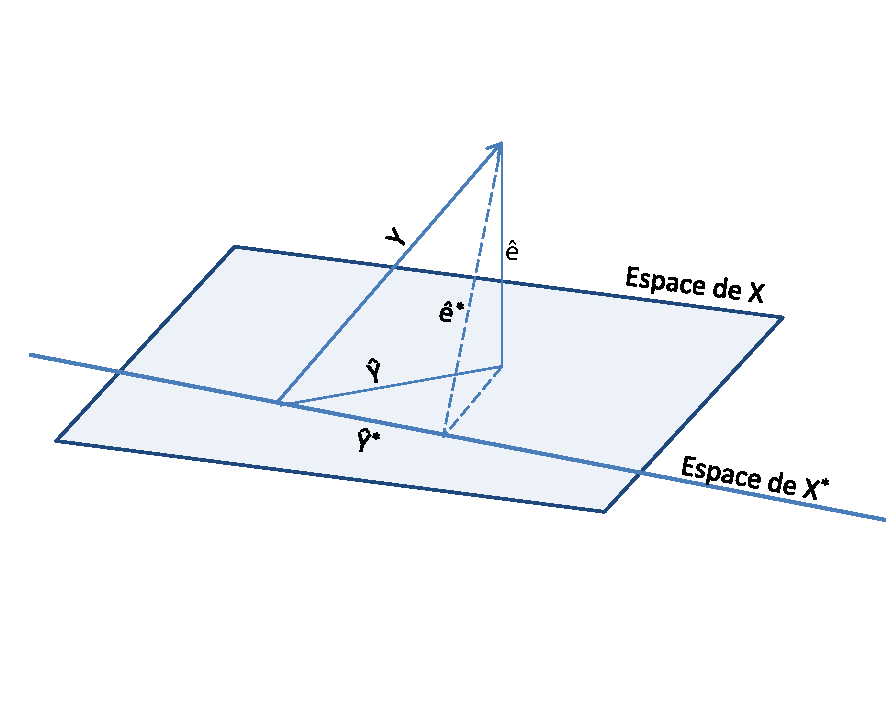
\includegraphics[scale = 0.8]{Chap6-InferenceRLM/Figures/geometrie_gen}
	\caption{Illustration de l'analyse de la variance généralisée}
	\label{fig:geometrie_gen}
\end{figure}

\begin{itemize}
\item[$\bullet$] Le plan Espace de $X$ est l'espace colonne de la matrice d'incidence sous $H_1$.
\item[$\bullet$] La droite Espace de $X^*$ est l'espace colonne de la matrice d'incidence sous $H_0$.
\item[$\bullet$] Le vecteur $\hY$ est $\boX\widehat{\bobeta}$ sous le modèle complet et se situe dans un espace de dimension $p'$. Ce vecteur constitue la projection orthogonale du vecteur
$\boY$ sur le plan nommé Espace de $X$.
\item[$\bullet$] Le vecteur $\boeps$ est constitué des résidus sous le modèle complet et vit dans un
espace de dimension $n-p'$.
\item[$\bullet$] Le vecteur $\hY^*$ représente le vecteur $\bold x^*\widehat{\bobeta}$ sous le modèle réduit et évolue dans un espace de dimension $p'-\Delta_{dl}$. Ce vecteur est la projection
orthogonale du vecteur $\boY$ sur la droite Espace de $X$.
\item[$\bullet$] Le vecteur $\boeps^*$ est formé des résidus sous le modèle réduit et
vit dans un espace de dimension $n-p'+\Delta_{dl}$.
\end{itemize}

Le vecteur égal à la différence entre les vecteurs de résidus des
deux mod\`eles est important. Notons $C$ sa longueur. $C^2$ est donc la différence entre les sommes
de carrés résiduels. Ce vecteur vit dans un espace de
dimension $\Delta_{dl}$. La statistique du test $F$ du principe de
somme de carrés résiduels additionnelle est tout simplement
égale \`a $(C^2/\Delta_{dl})/(B^2/(n-p'))$ où $B$ dénote la longueur du vecteur des résidus sous le modèle complet.

\section{Test d'une hypoth\`ese linéaire générale}
\label{sec:hyplingen}

Plusieurs tests en régression linéaire peuvent être exprimés comme une liste de contraintes linéaires sur les valeurs des param\`etres. Soit $\bo{C}$, une matrice de dimension
$r\times p'$, et $\bo{d}$, un vecteur de dimension $r\times1$. Un test d'hypoth\`ese linéaire
générale s'écrit comme
\begin{eqnarray}\label{H0:lingen}
H_0:~\bo{C}\bobeta&=&\bo{d}\\
H_1:~\bo{C}\bobeta&\neq&\bo{d}.\nonumber
\end{eqnarray}
On peut ré-écrire ce test d'hypoth\`ese sous la forme d'un mod\`ele réduit et d'un mod\`ele
complet de la manière suivante :
\begin{eqnarray*}
H_0:~\boY&=&\bo{Z}\bo{\alpha}+\boeps\\
H_1:~\boY&=&\boX\bobeta+\boeps,
\end{eqnarray*}
où l'équation en $H_0$ est obtenue en (i) résolvant le système d'équations
$\bo{C}\bobeta=\bo{d}$ pour $\bobeta$ et (ii) en substituant la solution trouvée en (i)
dans le modèle $\boY=\boX\bobeta+\boeps$.

%Puisque le test d'une hypothèse linéaire générale est équivalent à tester un modèle réduit contre un mod\`ele complet, on peut utiliser le principe de somme des carrés résiduels additionnelle.
Il est possible de
montrer \citep[voir par e.g.][pp. 44--45 et pp. 60--64]{Sen_Sri:90} que
$$SC_{res}^{(0)}-SC_{res}^{(1)}=(\bo{C}\widehat{\bobeta}-\bo{d})'[\bo{C}(\boX^\top\boX)^{-1}\bo{C}^\top]^{-1}(\bo{C}
\widehat{\bobeta}-\bo{d}).$$
Notez que $\sigma^2[\bo{C}(\boX^\top\boX)^{-1}\bo{C}^\top]$ est la variance de $\bo{C}\widehat{\bobeta}-\bo{d}$. Donc
la différence des sommes de carrés résiduels peut \^etre vue comme la longueur du vecteur
qui sépare $\bo{C}\widehat{\bobeta}$ et $\bo{d}$, standardisée par sa variance. Si la distance entre
$\bo{C}\widehat{\bobeta}$ et $\bo{d}$ est faible, alors $H_0$ constitue une hypothèse raisonnable, $SC_{res}^{(0)}-
SC_{res}^{(1)}$ prend une petite valeur et on ne rejette donc pas $H_0$. Si $H_0$ n'est pas réaliste, alors
$\bo{C}\widehat{\bobeta}$ sera éloignée de $\bo{d}$, $SC_{res}^{(0)}-SC_{res}^{(1)}$ prendra une grande valeur
et on rejettera l'hypothèse nulle $H_0$.

On peut maintenant construire la statistique $F$ en utilisant l'équation (\ref{F:ESS}):
\begin{equation*}\label{F:lingen}
F={(\bo{C}\widehat{\bobeta}-\bo{d})^\top[\bo{C}(\boX^\top\boX)^{-1}\bo{C}^\top]^{-1}(\bo{C}\widehat{\bobeta}-\bo{d})/r\over
SC^{(1)}_{res}/(n-p')}={
(\bo{C}\widehat{\bobeta}-\bo{d})^\top[\bo{C}(\boX^\top\boX)^{-1}\bo{C}^\top]^{-1}(\bo{C}\widehat{\bobeta}-\bo{d})\over
r\widehat\sigma^2_{H_1}},
\end{equation*}
où $r$ note le nombre de lignes de la matrice $\bo{C}$.
Le fait que $\Delta_{dl}=r$ dans ce cas est facile \`a comprendre si on utilise la troisième manière de le calculer, soit le nombre de contraintes sur les param\`etres du mod\`ele complet pour
obtenir le mod\`ele réduit. Sous l'hypothèse $H_0$, $F$ suit une loi de Fisher $\mathcal{F}_{r,n-p'}.$





\chapter{Variables catégoriques et interactions}\label{sec:CategoriquesInteractions}
\minitoc \mtcskip \minilof




Une grande différence quand on utilise un modèle de RLM au lieu de la RLS, c'est qu'on peut créer des modèles plus complexes. On verra ici deux façons pour ce faire, soit inclure des variables catégoriques et inclure des interactions.

\section{Variables exogènes catégoriques}

Jusqu'à maintenant, nous n'avons considéré que des variables
exogènes continues. Il arrive pourtant souvent en pratique que
les variables exogènes ne puissent prendre des valeurs que dans
un ensemble de valeurs possibles, et que ces valeurs n'impliquent
pas un ordre entre les mesures. Quelques exemples:
\begin{eqnarray*}
x_{1i}&=&\left\{\begin{array}{ll} H, & \mbox{si $i$ est un homme}\\
F, & \mbox{si $i$ est une femme}\end{array}\right.\\
x_{1i}&=&\left\{\begin{array}{ll} 1, & \mbox{si $i$ est une ville}\\
-1, & \mbox{si $i$ est un village}\end{array}\right.\\
x_{1i}&=&\left\{\begin{array}{ll}1, & \mbox{si $i$ est à ON}\\
0, & \mbox{si $i$ est à OFF}\end{array}\right.\\
\end{eqnarray*}

On peut simplement ajouter une variable catégorique linéairement dans le modèle de RLM. La valeur de cette variable modifiera l'ordonnée à l'origine de la régression. Il faut toutefois faire attention à la façon avec laquelle on code les variables catégoriques pour s'assurer que le modèle soit facile à interpréter.

\newpage
\textbf{Variable dichotomique}

Dans le cas d'une variable dichotomique, il est toujours plus prudent de coder $x_i$ sous la forme d'une variable indicatrice, c'est-à-dire sous la forme
$$x_i=\left\{\begin{array}{ll} 1, & \mbox{si ...}\\
0, & \mbox{sinon}\end{array}\right.$$

Si ce type de codage n'est pas utilisé, alors les $\beta$ peuvent \^etre difficiles à
interpréter.

Par exemple si
$$x_{i}=\left\{\begin{array}{ll}-5, & \mbox{si $i$ est un homme}\\
5, & \mbox{si $i$ est une femme}\end{array}\right.$$
Alors le modèle $Y_i=\beta_0+\beta_1 x_i+\varepsilon_i$ nous donne
\begin{eqnarray*}
\esp[Y_i|\mbox{$i$ est un homme}]&=&\beta_0-5\beta_1\\
\esp[Y_i|\mbox{$i$ est une femme}]&=&\beta_0+5\beta_1
\end{eqnarray*}
On a donc que $\beta_0$ est la moyenne des espérances de $Y$ pour les hommes et les femmes, et $\beta_1$ représente 0.1 fois la différence entre la valeur moyenne de $Y$ pour les hommes et celle pour les femmes.

Si on prend plutôt
$$x_{i}=\left\{\begin{array}{ll}1, & \mbox{si $i$ est un homme}\\
0, & \mbox{si $i$ est une femme}\end{array}\right.$$ alors on a
\begin{eqnarray*}
\esp[Y_i|\mbox{$i$ est un homme}]&=&\beta_0+\beta_1\\
\esp[Y_i|\mbox{$i$ est une femme}]&=&\beta_0
\end{eqnarray*}
et maintenant $\beta_0$ est simplement la valeur moyenne de $Y$ pour les femmes et  $\beta_1$ représente exactement la différence entre la valeur moyenne de $Y$ pour les hommes et celle pour les femmes.

Un autre codage souvent utilisé durant la collecte de données est de la forme

$$x_{i}=\left\{\begin{array}{ll}1, & \mbox{si $i$ est un homme}\\
2, & \mbox{si $i$ est une femme}\end{array}\right.$$

Dans ce cas, $\beta_1$ s'interprète de la même façon qu'avec la variable indicatrice, mais $\beta_0$ est plus complexe à interpréter.

\textbf{Variable polytomique}

Si $x$ est une variable polytomique, c'est-à-dire que $x_i$ peut
prendre une parmi $C\ge2$ valeurs possibles, la fa\c{c}on prudente
de procéder est de définir $C-1$ variables indicatrices.
Ainsi,
si $$x_{1i}=\left\{\begin{array}{ll} 1, & \mbox{si $i$ est bleu}\\
2, & \mbox{si $i$ est rouge}\\ 3, & \mbox{si $i$ est jaune}\\ 4, &
\mbox{si $i$ est vert}\end{array}\right.$$ alors on définit
\begin{eqnarray*}
x_{Bi}&=&\left\{\begin{array}{ll}1, & \mbox{si $i$ est bleu}\\ 0,
& \mbox{sinon}\end{array}\right.\ \ \
x_{Ri}=\left\{\begin{array}{ll}1, & \mbox{si
$i$ est rouge}\\ 0, & \mbox{sinon}\end{array}\right.\\
x_{Ji}&=&\left\{\begin{array}{ll}1, & \mbox{si $i$ est jaune}\\
0, & \mbox{sinon}\end{array}\right.\end{eqnarray*} Dans ce cas
\begin{eqnarray*}
x_{1i}=\mbox{bleu}&\Rightarrow&(x_{Bi},x_{Ri},x_{Ji})=(1,0,0)\\
x_{1i}=\mbox{rouge}&\Rightarrow&(x_{Bi},x_{Ri},x_{Ji})=(0,1,0)\\
x_{1i}=\mbox{jaune}&\Rightarrow&(x_{Bi},x_{Ri},x_{Ji})=(0,0,1)\\
x_{1i}=\mbox{vert}&\Rightarrow&(x_{Bi},x_{Ri},x_{Ji})=(0,0,0)
\end{eqnarray*}
Ainsi, si
$Y_i=\beta_0+\beta_{B}x_{Bi}+\beta_Rx_{Ri}+\beta_Jx_{Ji}+\varepsilon_i$,
\begin{eqnarray*}
\esp[Y_i|\mbox{$i$ est bleu}]&=&\beta_0+\beta_B\\
\esp[Y_i|\mbox{$i$ est rouge}]&=&\beta_0+\beta_R\\
\esp[Y_i|\mbox{$i$ est jaune}]&=&\beta_0+\beta_J\\
\esp[Y_i|\mbox{$i$ est vert}]&=&\beta_0.
\end{eqnarray*}


\begin{remarque}
Si une variable exogène ne prend que très peu de valeurs différentes, il est important de déterminer s'il s'agit d'une variable continue pour laquelle on a peu de mesures ou s'il
s'agit d'une variable polytomique. Selon la façon avec laquelle la variable est incluse dans le modèle, l'interprétation sera différente, ainsi que l'information qu'on pourra retirer du modèle.
\end{remarque}

\newpage
\begin{exemple}
\label{eg:lot}
Soit $x_{1i}$, le numéro de lot du produit $i$, $x_{2i}$, la
concentration de sel dans le produit $i$ et $Y_i$, l'indice de
qualité du produit $i$. Les variables $Y_i$ et $x_{2i}$ sont des
variables continues, alors que $x_{1i}$ est un variable
polytomique prenant une des valeurs $\{1,2,3,4\}$.

On ajuste le modèle
$$Y_i=\beta_0+\beta_{11}x_{11i}+\beta_{12}x_{12i}+\beta_{13}x_{13i}+\beta_2x_{2i}
+\varepsilon_i,$$ o\`u
\begin{eqnarray*}
x_{11i}&=&\left\{\begin{array}{ll} 1, & x_{1i}=1\\
0, & x_{1i}\neq1\end{array}\right. \ \ \
x_{12i}=\left\{\begin{array}{ll} 1, & x_{1i}=2\\
0, & x_{1i}\neq2\end{array}\right. \\
x_{13i}&=&\left\{\begin{array}{ll} 1, & x_{1i}=3\\
0, & x_{1i}\neq3.\end{array}\right.\end{eqnarray*}

La figure \ref{figex81} illustre graphiquement ce modèle. Notez qu'on suppose dans la figure que tous les coefficients sont positifs, mais ce n'est absolument pas nécessaire en pratique.

\begin{figure}[H]
\begin{center}
\centerline{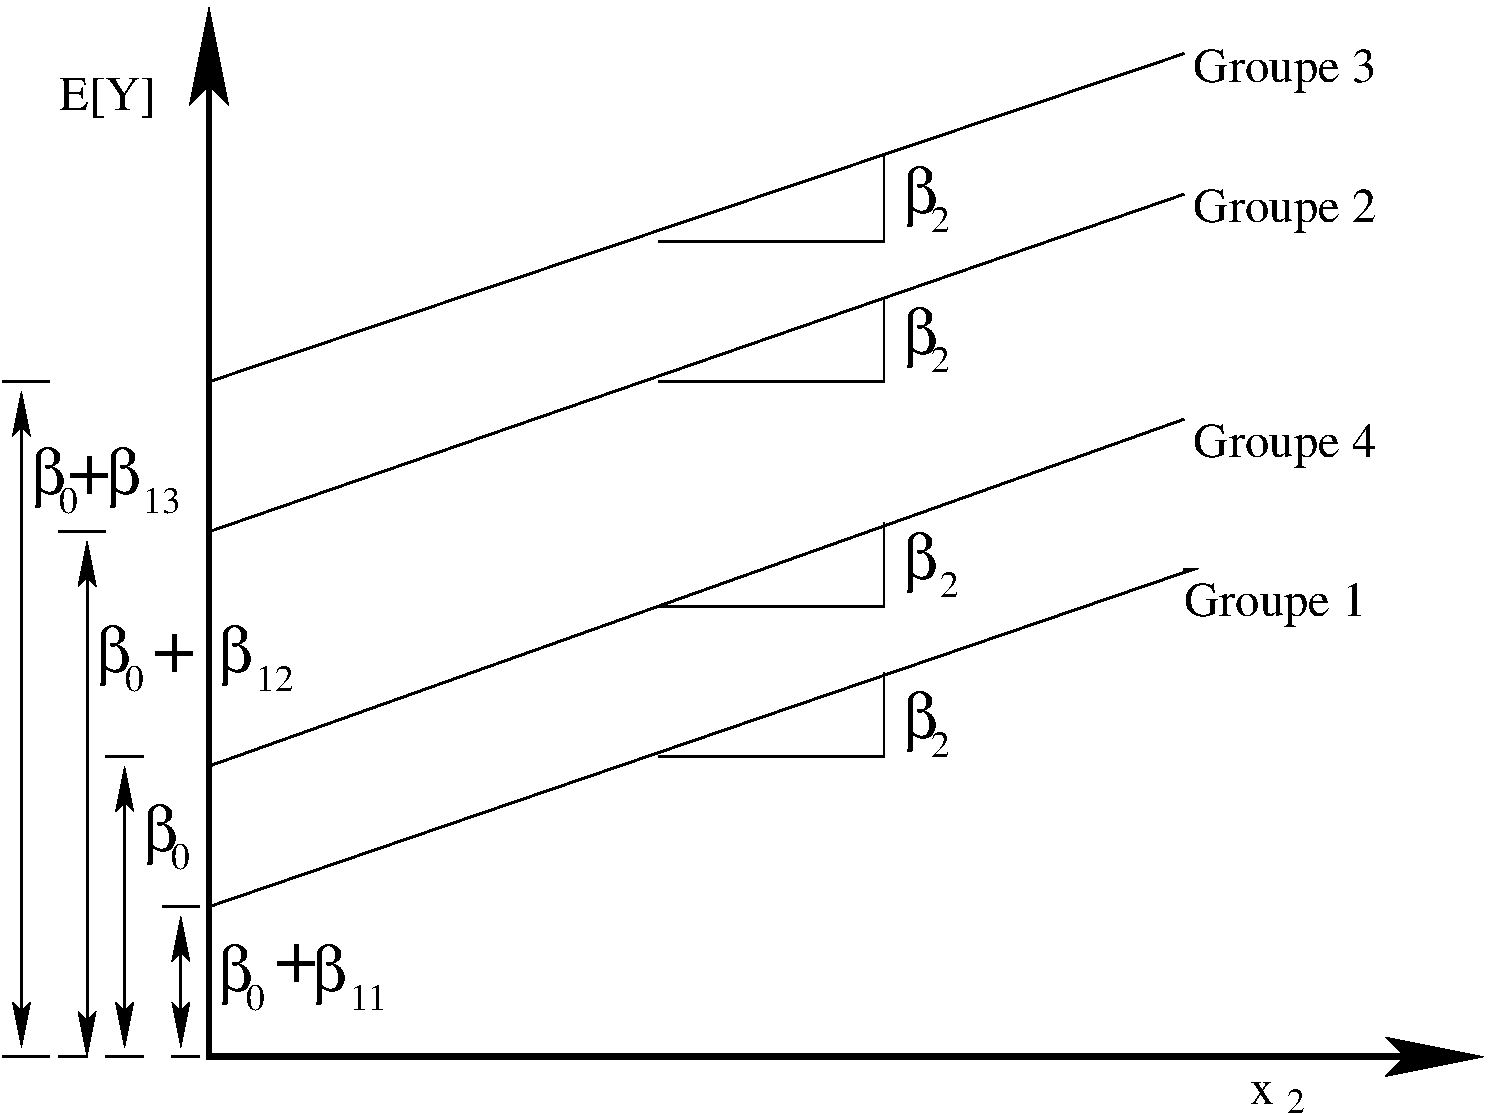
\includegraphics[height=3.5in,angle=0]{Chap7-CategoriquesInteractions/Figures/eyvsx2-eps-converted-to.pdf}}
\caption[Espérance de la variable endogène $Y$ en fonction de
la variable exogène $x_2$ pour chacun des groupes 1 à 4. ]{Espérance de la variable endogène $Y$ en fonction de
la variable exogène $x_2$ pour chacun des groupes 1 à 4. Comme on
peut le voir, les $\beta_0$ et $\beta_{1j}$ déterminent les
ordonnées à l'origine, tandis que $\beta_2$ détermine la
pente des droites de régression.}\label{figex81}
\end{center}
\end{figure}
\end{exemple}


\subsection{Inférence avec des variables catégoriques}

On peut en général faire de l'inférence sur les coefficients des variables indicatrices exactement comme pour les coefficients des variables continues.

\textbf{Tester l'utilité globale d'une variable polytomique}

Il faut toutefois faire attention si on veut tester si une variable polytomique possède un effet significatif
sur la valeur moyenne de la variable endogène. On doit alors tester si
plusieurs coefficients sont simultanément égaux à zéro à
l'aide d'un test $F$ de réduction de modèle. En général, pour tester si une variable polytomique prenant
$C$ valeurs possibles a un effet significatif, il faut tester si
$C-1$ coefficients sont simultanément égaux à zéro.

\begin{exemple}
Supposons que dans le modèle de l'exemple \ref{eg:lot} on souhaite tester si le groupe
d'o\`u provient l'item $i$ a un effet sur la variable dépendante. Il faut alors tester $H_0:\beta_{11}=\beta_{12}=\beta_{13}=0$. Notez que ceci revient à tester si la droite de régression est la m\^eme pour les 4 groupes, c'est-à-dire que sur la figure
\ref{figex81}, les 4 lignes sont superposées.
\end{exemple}

\textbf{Tester une hypothèse plus complexe sur les différents niveaux d'une variable}


Notons aussi que plusieurs hypothèses intéressantes dans un modèle avec variables polytomiques peuvent \^etre vues comme des hypothèses linéaires sur les $\beta$, ce qui nous permet d'utiliser nos résultats de la section \ref{sec:hyplingen}.

\begin{exemple}
Toujours pour le modèle de l'exemple \ref{eg:lot}, supposons qu'on veut tester que la valeur moyenne de $Y_i$ est la m\^eme pour les lots 1 et 3. Ceci revient à tester si $\beta_{11} = \beta_{13}$. On peut donc utiliser un test d'hypothèse linéaire générale avec $$\bo{C} = (0,1,0,-1,0).$$
On pourrait aussi vouloir tester si on peut diviser les lots en deux : les lots 1 et 3 ayant la même moyenne, et les lots 2 et 4 ayant la même moyenne. Ici encore, c'est un test d'hypothèse linéaire générale, mais avec deux contraintes simultanées. La matrice C appropriée est alors:

$$ \bo{C}  =
\begin{bmatrix}
    0 & 1 & 0 & -1 & 0 \\
    0 & 0 & 1 & 0 & 0
\end{bmatrix}.
$$
\end{exemple}




\section{Interactions}

Une interaction entre deux variables exogènes $x_{1i}$ et $x_{2i}$ est un terme de la forme $$\beta_{12}x_{1i}x_{2i}.$$ On inclut une interaction dans un modèle lorsque l'effet d'une des variables sur la moyenne de $Y$ dépend de la valeur d'une autre variable. En effet, supposons le modèle
\vspace{-0.05in}
\begin{equation*}
Y_i=\beta_0+\beta_1x_{1i}+\beta_2x_{2i}+\beta_{12}x_{1i}x_{2i}+
\varepsilon_i.
\end{equation*}
On a alors
\vspace{-0.05in}
\begin{eqnarray}
\esp[Y_i|x_{1i}+1]&=&\beta_0+\beta_1(x_{1i}+1)+\beta_2x_{2i}+\beta_{12}(x_{1i}+1)x_{2i}\label{eq:interaction1}\\
\esp[Y_i|x_{1i}]&=&\beta_0+\beta_1x_{1i}+\beta_2x_{2i}+\beta_{12}x_{1i}x_{2i}.\label{eq:interaction2}
\end{eqnarray}
L'effet d'une augmentation d'une unité de $x_{1i}$ sur $\esp[Y_i]$ est
$\beta_1+\beta_{12}x_{2i}$, c'est-à-dire que l'effet d'une augmentation
de $x_{1i}$ d'une unité sur $\esp[Y_i]$ \textbf{dépend de la valeur
de $x_{2i}$}.

%Alors que l'inclusion d'une variable catégorique dans le modèle modifie l'ordonnée à l'origine, l'inclusion d'une interaction modifie plutôt la pente de la droite ou de l'hyperplan.

\begin{exemple}\label{ex83}
Soit $x_{1i}$ une variable polytomique pouvant prendre les valeurs
$\{1,2,3\}$ et soient $x_{11i}$ l'indicatrice que $x_{1i}=1$ et
$x_{12i}$ l'indicatrice que $x_{1i}=2$. Le modèle
$$Y_i=\beta_0+\beta_{11}x_{11i}+\beta_{12}x_{12i}+\beta_2x_{2i}
+\beta_{112}x_{11i}x_{2i}+\beta_{122}x_{12i}x_{2i}+\varepsilon_i.$$
est illustré à la figure \ref{figex83}.
%Les $\beta_0$ et $\beta_{1ji}$ déterminent les ordonnées à l'origine, tandis que $\beta_2$ et $\beta_{1j2}$ déterminent les pentes des droites de régression.
\begin{figure}[H]
\begin{center}
\centerline{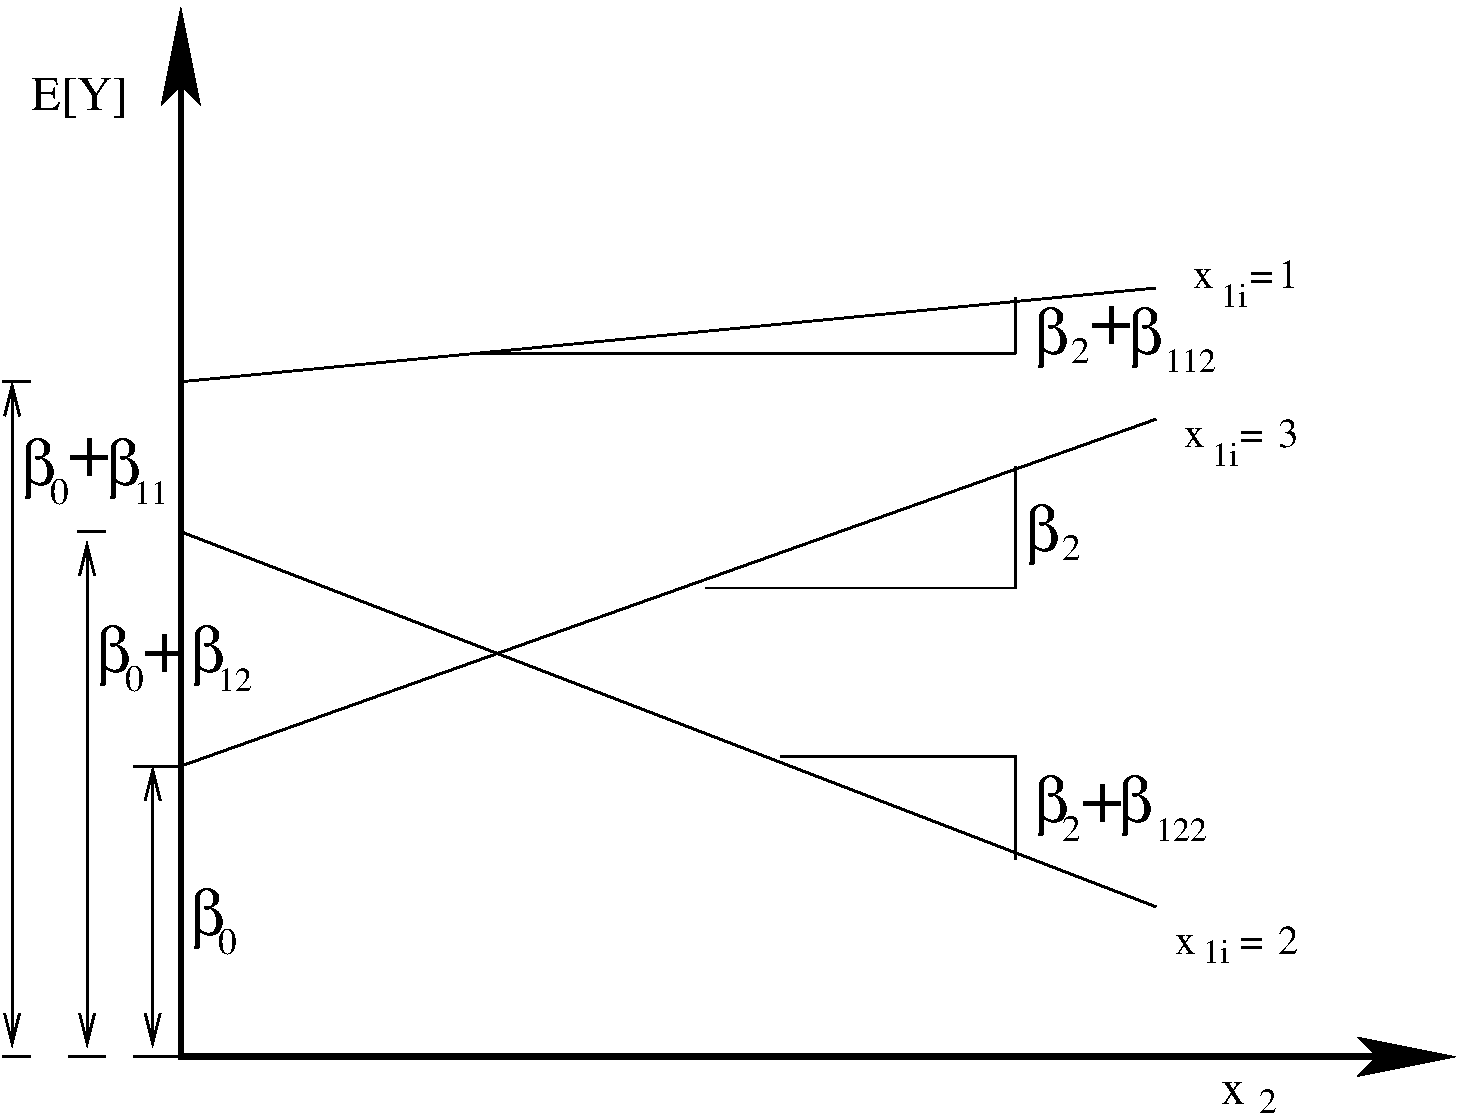
\includegraphics[scale = 0.35]{Chap7-CategoriquesInteractions/Figures/eyvsx2b-eps-converted-to.pdf}}
\caption{Espérance de la variable endogène $Y$ en fonction de
la variable exogène $x_2$ pour chacune des valeurs de $x_{1i}$.
}\label{figex83}
\end{center}\end{figure}
\end{exemple}



L'exemple \ref{ex83} illustre une interaction entre une variable catégorique et une variable continue, ce qui s'illustre aisément. On peut également inclure une interaction entre deux variables catégoriques, ce qui crée en quelque sorte une nouvelle variable catégorique avec plus de catégories. Ou entre deux variables continues, ce qui implique une pente de régression pour une première variable qui diffère pour chaque valeur d'une autre variable.

De plus, les termes d'interaction ne sont pas limités à seulement deux variables. En effet, si nous mesurons 4 variables $x_1,\ldots,x_4$
il se pourrait que le modèle approprié soit
\begin{eqnarray*}
Y_i&=&\beta_0+\beta_1x_{1i}+\beta_2x_{2i}+\beta_3x_{3i}+\beta_4x_{4i}+
\beta_{12}x_{1i}x_{2i}+\beta_{13}x_{1i}x_{3i}\\
&\ &\ \ \ +\beta_{14}x_{1i}x_{4i}+\beta_{23}x_{2i}x_{3i}+
\beta_{24}x_{2i}x_{4i}+\beta_{34}x_{3i}x_{4i}\\
&\ &\ \ \ +\beta_{123}
x_{1i}x_{2i}x_{3i}+\cdots+\beta_{1234}x_{1i}x_{2i}x_{3i}x_{4i}
+\varepsilon_i.\end{eqnarray*} Mais à moins de posséder vraiment beaucoup
de données, les interactions impliquant plus de deux variables
sont rarement utilisées. Elles sont en outre plus complexes à interpréter.


\subsubsection*{Test de linéarité}

Pour tester si un modèle est adéquat, on peut y ajouter des
termes d'interaction et tester si ces termes sont significatifs.
\begin{exemple}
Soit le modèle
$$Y_i=\beta_0+\beta_1x_{1i}+\beta_2x_{2i}+\varepsilon_i.$$ Nous pouvons tester si
$H_0:\ \beta_{12}=0$ contre $H_1:\ \beta_{12}\neq0$ à partir du
modèle
$$Y_i=\beta_0+\beta_1x_{1i}+\beta_2x_{2i}+\beta_{12}x_{1i}x_{2i}+\varepsilon_i.$$
Si nous ne rejetons pas $H_0$, les données ne fournissent pas de preuve suffisante en faveur de cette interaction; cela ne démontre pas que le modèle est adéquat. Si nous rejetons $H_0$, alors le
modèle sans interaction n'est pas adéquat.\\
\end{exemple}

\begin{remarque}
Un cas particulier d'interaction est si on inclut une interaction entre une variable $x_j$ et elle-même, ce qui crée un terme de la forme $x_j^2$ dans l'équation de régression. Ce peut être utile si la relation entre les variables est quadratique plutôt que linéaire. On y reviendra à la section \ref{sec:regpoly}.
\end{remarque} 

\chapter{Choix de modèle pour la RLM}\label{sec:ChoixModeleRLM}
\minitoc \mtcskip \minilof
%


Comme pour la RLS, il est important lors du choix de modèle de s'assurer que les postulats sont bien respectés. Une autre difficulté de la RLM est qu'il faut choisir les variables à inclure dans le modèle parmi toutes celles à notre disposition. Nous abordons ces deux étapes dans ce chapitre.

\section{Vérification des postulats et transformations}

L'analyse des résidus pour la RLM est très similaire à celle des résidus pour la RLS. Nous révisons ici brièvement les diagnostics de régression, et introduisons quelques nouvelles procédures.

\subsection{Les résidus}

Comme pour la RLS, le résidu est l'outil de base pour la vérification des postulats. On a déjà vu à la section \ref{sec:distYhatEps} que $\hboeps=\boY-\hY=(\boI_n-\boH)\boY$ et que
\begin{eqnarray*}
	\hboeps \sim \N_n(0, \sigma^2(\boI_n-\boH)).
\end{eqnarray*}

Tout comme pour la RLS, les résidus suivent une loi normale de moyenne $\boz$, mais ne sont pas indépendants et n'ont pas des variances homogènes.

Les résidus standardisés et studentisés sont définis exactement comme pour la RLS:

$$r_i = \dfrac{\hat\varepsilon_i}{\sqrt{\hat\sigma^2(1-h_{ii})}}
\hspace{1cm}
t_i={\hat\varepsilon_i\over \hat{\sigma}_{(i)} \sqrt{1-h_{ii}}}$$


%La plupart des graphiques du Chapitre 2 sont toujours très utiles pour la validation des postulats du modèle et s'interprètent de la m\^eme fa\c{}con qu'auparavant.  Nous traiterons dans les sections suivantes quelques \'etapes de validation d'un modèle de r\'egression lin\'eaire multiple.

\subsection{Vérification de la linéarité}

On peut utiliser les mêmes graphiques que pour la RLS. On doit notamment observer le graphique de  $\hboeps$ \textit{versus} $x_j$ pour toutes les variables explicatives. On pourra alors identifier la ou les variables pour lesquelles la relation avec $Y$ n'est pas linéaire, et corriger le problème par une transformation appropriée.

% Ces graphiques devraient ne montrer aucune tendance, avec les résidus symétriques autour de zéro en ordonnée et une variabilité qui ne varie pas beaucoup en fonction de la valeur de $x_ji$. \vspace{1mm}

Toutefois, \textbf{les graphiques à variable ajoutée} sont mieux adaptés au contexte de la régression multiple pour détecter le manque de linéarité. Un graphique à variable ajoutée est un nuage de points de $\hboeps_{\boY|\boX_{-j}}$ vs $\hboeps_{x_j|\boX_{-j}}$. Ici $\hboeps_{\boY|\boX_{-j}}$ représente le vecteur des
résidus obtenu en régressant $\boY$ sur toutes les variables
exogènes du modèle \textbf{excepté} $x_j$. Il s'agit donc de la partie des $Y_i$ qui n'est pas expliquée par l'ensemble des variables exogènes, sauf la variable d'intérêt.  On veut ensuite savoir si ajouter la variable $x_j$ permet d'expliquer davantage les $Y_i$.  On pourrait tout simplement regarder la relation entre $x_j$ et $\hboeps_{\boY|\boX_{-j}}$, mais puisque $x_j$ peut lui-même être expliqué par les autres variables exogènes, il faut être un peu plus rusé. On utilise donc $\hboeps_{x_j|\boX_{-j}}$, soit le vecteur des résidus de la régression avec $x_j$ comme variable endogène et toutes les variables explicatives sauf $x_j$ comme variables exogènes. On l'obtient en ajustant le modèle suivant:
\begin{equation*}
  x_{ij} = \delta_0+\delta_1x_{i1}+...+\delta_px_{ip} +\varepsilon_{i\,[x_j|\boX_{-j}]}.
\end{equation*}
Plus les résidus de cette régression sont grands, plus $x_j$ ajoute de l'information importante au modèle.

Le nuage de points de $\hboeps_{\boY|\boX_{-j}}$ vs $\hboeps_{x_j|\boX_{-j}}$ tombera dans un des trois cas suivants:
\begin{itemize}
\item Si $x_j$ est vraiment une variable qui entre linéairement dans le modèle, \\
 le graphique devrait donner une droite de pente $\beta_j$ passant par l'origine.
\item  Si $x_j$ est \og inutile \fg, \\
le graphique devrait ressembler à un graphique de
résidus ordinaires.
\item  Si $x_j$ est utile mais entre dans le modèle de fa\c{}con non linéaire,\\
 le graphique devrait avoir l'allure d'une courbe plut\^ot que d'une droite.  On pourra donc détecter le manque de linéarité en $x_j$ de la moyenne de $\boY$.
\end{itemize}

\vspace{0.05 in}
Dans certains cas, il est également possible de tester la linéarité d'un modèle à l'aide d'un test de manque d'ajustement. Nous présentons celui-ci à la section \ref{sec:testAjustement}.

\newpage

\subsection{Homogénéité des variances}

On teste l'homogénéité des variances avec le graphique $r_i$ vs $\hat{Y}_i$ comme pour la RLS. S'il y a un problème, on tentera souvent de le régler en transformant la variable endogène.

Notons également qu'il existe un test formel de l'homogénéité des variances, soit le test de \citet{Whi:1980}. La statistique du test de White s'exprime comme suit
$$\chi^2_{\text{White}} = nR^2 \overset{a}{\sim} \chi^2_{p(p+3)/2}$$
o\`u $R^2$ est le coefficient de détermination ($R^2$) de la régression de $\hat\varepsilon_i^2$ sur toutes les variables explicatives $x_j$, de m\^eme que sur tous les produits croisés entre ces variables, incluant le carré de chacune des variables. On rejette l'hypothèse d'homogénéité des variances au seuil
$\alpha$ lorsque $\chi^2_{\text{White}}>\chi^2_{p(p+3)/2;1-\alpha}$.

\subsection{Normalité des erreurs}

Les mêmes outils que pour la RLS peuvent être utilisés pour tester la normalité des erreurs. Quand le postulat de normalité n'est pas rencontré, il peut \^etre souhaitable  d'utiliser la technique de transformation de Box-Cox (voir section \ref{sec:LaTechniqueDeBoxCox}) pour déterminer la meilleure transformation de la variable endogène.

Il vaut la peine de noter que le test de Shapiro-Wilk est très puissant et que
pour de gros échantillons, il rejettera très souvent la
normalité. Comme les seuils des tests $t$ de Student et $F$ de Fisher ne sont pas
sérieusement affectés si la distribution des résidus est
près de la normalité sans l'atteindre exactement, alors il est
toujours bon d'accompagner le test de normalité d'un diagramme quantile-quantile pour s'assurer que la non-normalité est vraiment sérieuse.

\subsection{Transformation de Box-Cox}
\label{sec:LaTechniqueDeBoxCox}
Pour une réponse strictement positive, on peut considérer la famille
\[
 g_\lambda(Y)=\begin{cases}(Y^\lambda-1)/\lambda,&\lambda\ne0,\\
 \log(Y),&\lambda=0.\end{cases}
\]
On choisit une transformation en tenant compte de la vraisemblance avec son
jacobien, de l'interprétation et des diagnostics du modèle transformé.
Une transformation ne corrige pas automatiquement tous les problèmes.
L'inverse de la moyenne prédite sur l'échelle transformée n'est généralement
pas la moyenne sur l'échelle originale. Il faut tenir compte de ce biais
lorsqu'on souhaite prédire une moyenne sur l'échelle originale.

\subsection{Indépendance des erreurs}

On vérifie l'indépendance des erreurs exactement de la même façon que pour la RLS. Si les données sont chronologiques, on peut utiliser un graphique des résidus versus le temps. Sinon, il faut se fier à la description de la collecte de données.

\newpage
\subsection{Test pour manque d'ajustement (lack-of-fit)}
\label{sec:testAjustement}

Ce test permet de vérifier si le modèle proposé s'ajuste bien
aux données. Il constitue un bon complément à l'analyse des
résidus. Toutefois, ce test ne peut être utilisé que lorsque nous avons plusieurs observations dont la (les) variable(s) exogène(s) a (ont) exactement la (les) m\^eme(s) valeur(s).

\begin{exemple}
\label{lof1}
Le tableau \ref{jeuLOF} montre un jeu de données où les observations 2 et 3, 4 et 5 et 7 et 8 ont les m\^emes combinaisons de valeurs pour leurs variables exogènes. Un test de manque d'ajustement est donc possible dans ce cas.

\begin{table}[H]
\begin{center}
\begin{tabular}{||cccc||cccc||}\hline\hline
Obs & $Y_i$ & $x_{1}$ & $x_{2}$ & Obs & $Y_i$ & $x_{1}$
& $x_{2}$ \\ \hline\hline
 1 &  8.74 & 2 & 1 &&&& \\
 2 & 7.10 & 2 & 0 & 3 & 9.85 & 2 & 0 \\ 4 & 12.1 & 5 & 1 & 5 & 13.1 & 5 & 1 \\
 6 & 14.1 & 5 & 0 &&&& \\
 7 & 18.6 & 8 & 1 & 8 & 15.0 & 8 & 1 \\
 9 & 16.9 & 8 & 0 &&&& \\
\hline\hline
\end{tabular}\end{center}
\caption{Jeu de données pour lequel le test de manque d'ajustement s'applique.}
\label{jeuLOF}
\end{table}
\end{exemple}

Le test de manque d'ajustement se base sur le fait qu'on peut estimer $\sigma^2$ (l'erreur pure) gr\^ace à la variabilité de la variable endogène parmi les observations ayant une m\^eme combinaison de variables exogènes. On peut ainsi séparer notre somme de carrés résiduels en une partie due à l'erreur pure et une partie due au manque d'ajustement du modèle. Mathématiquement, on écrira
$$
{\underbrace{\sum_{k=1}^m\sum_{j=1}^{n_k}(Y_{kj}-\hat{Y}_k)^2}\atop
SC_{res}}={\underbrace{\sum_{k=1}^m\sum_{j=1}^{n_k}(Y_{kj}-\overline{Y}_k)^2}
\atop
SC_{pure}}+{\underbrace{\sum_{k=1}^mn_k(\overline{Y}_k-\hat{Y}_k)^2}
\atop SC_{ajust.}}.$$
o\`u
\begin{itemize}
\item[$\bullet$] $m$ est le nombre de combinaisons distinctes des valeurs des variables exogènes
\item[$\bullet$] $n_k$, le nombre d'observations de la $k^e$ combinaison de variables exogènes
\item[$\bullet$] $Y_{kj}$ la $j^e$ observation de la variable endogène pour la $k^e$ combinaison de variables exogènes
\item[$\bullet$] $\overline{Y}_k=\sum_jY_{kj}/{n_k}$, la valeur moyenne de la variable
endogène pour la $k^e$ combinaison de variables exogènes
\end{itemize}



%La variabilité dans les $Y_i$ peut maintenant \^etre estimée à partir des données ayant les m\^emes combinaisons pour les variables exogènes, et ce m\^eme sans modèle: $$s^2={\sum_{i=1}^m\sum_{j=1}^{n_i}(Y_{ij}-\overline{Y}_i)^2\over\sum_{n_i-1}}.$$


Si le modèle de régression est adéquat, alors $\hat{Y}_k$ sera une bonne estimation de la vraie moyenne de $Y$ pour la $k^e$ combinaison de variables exogènes. Dans ce cas, $\overline{Y}_k$ sera proche de la valeur prédite $\hat{Y}_k$ et la $SC_{ajust.}$ sera petite. On compare $SC_{ajust.}$ à $SC_{pure}$ pour tester l'adéquation du modèle.

On teste donc les hypothèses

$H_0 : E(Y_i) = \beta_0 + \beta_1 x_1 + \ldots \beta_p x_p$ \\
$H_1 : E(Y_i) \ne \beta_0 + \beta_1 x_1 + \ldots \beta_p x_p$

On procède alors à une analyse de variance, résumée au tableau \ref{tab:anovaLOF}.

\begin{table}[H]
\centering
\begin{tabular}{|c||c|c|c|c|}\hline\
 & dl & SC & CM & $F$  \\ \hline\hline
 Manque &  $m-p'$ & $SC_{ajust.}$ &    $\frac{SC_{ajust.}}{m-p'}$  &     ${SC_{ajust.}/(m-p')\over SC_{pure}/(n-m)}$   \\
 d'ajustement & & & &  \\
 Erreur pure  & $n-m$ & $SC_{pure}$ &   $\frac{SC_{pure}}{n-m}$  & \\
 Erreur totale & $n-p'$ & $SC_{res}$ &    &  \\ \hline
\end{tabular}
\caption{Table d'ANOVA pour un test de manque d'ajustement}
\label{tab:anovaLOF}
\end{table}

On rejette $H_0$ si  $F \ge F_{m-p',n-m,\;1-\alpha}$. On peut également obtenir une valeur de $p$ en comparant notre statistique $F$ à la distribution $F_{m-p',n-m}$.

\vspace{0.05in}
\begin{exemple}
Dans les données de l'exemple \ref{lof1}, on a $m=6$ combinaisons de valeurs différentes pour $(x_{1i},x_{2i})$: $\{ (2,1),(2,0),  (5,1), (5,0), (8,1),(8,0)\}$. \\
On a par exemple $n_2=2$ observations avec $(x_{1i},x_{2i})=(2,0)$, et $\overline{Y}_2=8.475$.\\
On peut calculer les 5 autres moyennes pour obtenir $SC_{pure}$.

On ajuste également le modèle $Y_{ij}=\beta_0+\beta_1x_{1i}+\beta_2x_{2i}+\varepsilon_{ij}$, et on obtient alors $\hat{Y}_1, \ldots, \hat{Y}_6$, ce qui permet de calculer $SC_{res}$ et $SC_{ajust.}$. On trouve:

\begin{center}
\begin{tabular}{||c||c|c|c|c|c||}\hline\hline
  & dl & SC & CM & F & $Pr>F$ \\ \hline\hline
 Manque ajustement &  3 &    1.598029 &    0.53267  &     0.1484   &
 0.9242 \\
 Erreur pure  &  3 &   10.76125 &    3.58708  & & \\
 Erreur totale &  6 &   12.3598 &   2.0599   & & \\ \hline\hline
\end{tabular}
\vspace{5mm}
\end{center}

\vspace{-0.05in}
Il ne semble pas y avoir de problème de manque d'ajustement dans notre exemple. Bien entendu, avec le très petit nombre de données observé, très peu d'hypothèses peuvent \^etre rejetées!
\end{exemple}

\newpage
\section{Importance de la sélection de variables}

Pour la RLM, la vérification des postulats n'est pas le seul élément important dans le choix du modèle. Il faut aussi sélectionner les variables à inclure dans le modèle.

En effet, il se peut que certaines variables dans notre jeu de données de soient pas associées à la variable réponse.
%On verra à la section \ref{sec:inclurevar} qu'il est important d'inclure toute les variables utiles, et seulement celles-ci.
En présence d'un grand nombre de variables exogènes, on court deux dangers: enlever une variable qui est utile pour expliquer la variable endogène, et conserver dans le modèle une variable qui n'est pas utile.

\textbf{Conserver une variable inutile}

Si on conserve trop de variables, on va augmenter inutilement la variance des estimations. Par conséquent, certains effets importants risquent d'être jugés non significatifs.

Plus précisément, supposons que le bon modèle soit:
\begin{eqnarray}
% \nonumber to remove numbering (before each equation)
Y_i &=& \beta_0+\beta_1 x_{1i}+...+\beta_k x_{ki}+ \varepsilon_i.
\label{eq:modelekvar}
\end{eqnarray}
Si on ajoute la variable $x_{k+1}$ et qu'on ajuste le modèle:
\begin{eqnarray}
% \nonumber to remove numbering (before each equation)
\label{eq:modelekplus1var}
  Y_i &=& \beta_0^*+\beta_1^* x_{1i}+...+\beta_k^* x_{ki}+ \beta_{k+1}^* x_{(k+1)i}+ \varepsilon_i
\end{eqnarray}

on obtiendra que $$\var[\hat\beta^*_j] \geq \var[\hat\beta_j],\qquad\text{pour } \;j=1,...,k.$$
De plus, la prévision faite pour $Y$ en un $\bo{x}^*$ donné sera moins précise avec le modèle superflu de l'équation \eqref{eq:modelekplus1var} qu'avec le modèle simple de l'équation \eqref{eq:modelekvar}.

\textbf{Enlever une variable utile}

À l'opposé, si on enlève trop de variables, le modèle sera biaisé. Pour illustrer le biais, prenons par exemple les deux modèles suivants exprimés sous forme matricielle :
\begin{eqnarray}
% \nonumber to remove numbering (before each equation)
  \boY &=& \boX_1\bobeta_1 + \boeps,
  \label{eq:1parametre}
  \end{eqnarray}
  \begin{eqnarray}
  \boY &=& \boX_1\bobeta_1 +\boX_2\bobeta_2 +\boeps,
  \label{eq:2parametres}
\end{eqnarray}
où $\bobeta_1$ comporte $p'=p+1$ paramètres et $\bobeta_2$ inclut $m-p'$ paramètres.

Supposons que le bon modèle soit celui de l'équation \eqref{eq:2parametres} et qu'on choisisse plutôt le modèle de l'équation \eqref{eq:1parametre}, on aura alors
\begin{eqnarray*}
% \nonumber to remove numbering (before each equation)
  \esp[\hbobeta_1] &=& (\boX_1'\boX_1)^{-1}\boX_1'\esp[\boY] \\
  &=&  (\boX_1'\boX_1)^{-1}\boX_1' (\boX_1\bobeta_1 + \boX_2\bobeta_2)\\
  &=& \bobeta_1 + (\boX_1'\boX_1)^{-1}\boX_1'\boX_2 \bobeta_2.
\end{eqnarray*}
On a donc que $\hbobeta_1$ est un estimateur biaisé.

Si l'on s'intéresse plutôt à la prévision au point $\bo{x}^* = \left[\begin{array}{cc}\bo{x}_1^*\\\bo{x}_2^*\end{array}\right]$, le modèle à $p'$ paramètres nous donnerait
\begin{eqnarray*}
% \nonumber to remove numbering (before each equation)
   \hY(\bo{x}_1^{*}) &=& \bo{x}_{1}^{*'} \hbobeta_1 \\
  \esp[\hY(\bo{x}_1^{*})] &=& \bo{x}_{1}^{*'} \esp[\hbobeta_1]  \\
     &=& \bo{x}_{1}^{*'} \{\bobeta_1 + (\boX_1'\boX_1)^{-1}\boX_1'\boX_2 \bobeta_2\}
\end{eqnarray*}
alors que le modèle à $m$ paramètres conduirait à
\begin{eqnarray*}
   \hY(\bo{x}^{*}) &=& \bo{x}_{1}^{*'} \hbobeta_1^* + \bo{x}_{2}^{*'}\hbobeta_2^* \\
  \esp[\hY(\bo{x}^{*})] &=&  \bo{x}_{1}^{*'} \bobeta_1 + \bo{x}_{2}^{*'}\bobeta_2.
\end{eqnarray*}

Le biais dans la prévision serait donc
\begin{eqnarray*}
% \nonumber to remove numbering (before each equation)
   \mbox{biais}[\hY(\bo{x}^{*})]&=&  \esp[\hY(\bo{x}_1^{*})] -\esp[\hY(\bo{x}^{*})]\\
   &=& \bo{x}_{1}^{*'} \{\bobeta_1 + (\boX_1'\boX_1)^{-1}\boX_1'\boX_2 \bobeta_2\} -  \bo{x}_{1}^{*'} \bobeta_1 - \bo{x}_{2}^{*'}\bobeta_2\\
   &=& [{\bo{x}_{1}^{*'}(\boX_1'\boX_1)^{-1}\boX_1'\boX_2}-\bo{x}_{2}^{*'}]\bobeta_2.
\end{eqnarray*}

\textbf{En somme}

En résumé, un trop grand nombre de variables mène à une variance trop grande et un trop petit nombre de variables conduit à une estimation biaisée. Il est donc important de chercher un ensemble de variables permettant d'atteindre un compromis entre ces deux critères. Pour ce faire, on a souvent recours à l'une des techniques de sélection de variables pour choisir un sous-ensemble raisonnable de variables.

\newpage

\section{Critères basés sur l'ajustement du modèle}

Pour sélectionner les bonnes variables dans le modèle, plusieurs techniques sont disponibles. Voyons d'abord quelques critères basés sur l'ajustement du modèle.

\subsection{Coefficient de détermination}

Comme pour la RLS, le coefficient de détermination est défini comme
\begin{equation}\label{R^2}
R^2={SC_{reg}\over SC_{tot}}=1-{SC_{res}\over SC_{tot}}.
\end{equation}

C'est une mesure d'ajustement du modèle facile à calculer et à interpréter, mais il est problématique pour la RLM puisque sa valeur ne peut jamais diminuer si on ajoute une variable dans le modèle, même si celle-ci est inutile.

En effet, si on ajoute un terme à un modèle de régression, $SC_{reg}$ ne peut pas diminuer. Comme $SC_{tot}$ ne dépend pas du modèle, elle reste inchangée. Donc l'ajout d'un terme au modèle se traduit forcément par un $R^2$ plus grand.
%Ainsi, si le ``vrai" modèle générant les données est $Y_i=\beta_0+\beta_1x_{i1}+\varepsilon_i$ et que l'on ajuste ce modèle ainsi que le modèle $Y_i=\beta_0+\beta_1x_{i1}+\beta_2x_{i2}+\varepsilon_i$, il est fort probable que le $R^2$ du second modèle soit supérieur à celui du ``vrai" modèle.
L'ajout de termes superflus réduit en général la précision dans les prévisions, ce qu'on souhaite éviter. Le coefficient de détermination n'est donc pas utile pour la RLM.

\subsection{Coefficient de détermination ajusté}

Il s'agit d'un coefficient de détermination qui pénalise pour l'ajout d'un trop grand nombre de variables. Plus précisément, il est défini comme :
\begin{equation}\label{R^2a}
R^2_{a}=1-{CM_{res}\over CM_{tot}}=1-{SC_{res}/(n-p')\over
SC_{tot}/(n-1)}=1-{(n-1)\hat\sigma^2\over SC_{tot}}.
\end{equation}
Avec $R^2_{a}$, l'ajout d'une variable exogène peut aussi
résulter en une diminution de la statistique.
%Tout comme
%c'était le cas pour $R^2$, la valeur maximale que peut prendre
%$R^2_{ajus}$ est 1.
Comme on peut le voir dans la dernière
égalité de l'équation (\ref{R^2a}), comparer deux
modèles sur la base de leur $R^2_{a}$ est équivalent à
comparer deux modèles sur la base de leur estimation de la
variance des termes d'erreur $\hat\sigma^2$, puisque $SC_{tot}$ et $n$ ne
dépendent pas du modèle choisi.

Notez que peu importe si on utilise $R^2$ ou $R^2_{a}$, on ne peut pas vraiment se fier sur ces statistiques pour comparer des modèles employant des transformations différentes de la variable endogène, ou un modèle avec et un modèle sans ordonnée à l'origine.


\subsection{Critère d'information d'Akaike (AIC)}

%%%%%%%%%%%%%%%%%%%%%%%%%%%%%%%%%%%%%%%%%%%%%%%%%%%%%%%%%%%%%%
% Je crois que les commandes AIC et BIC dans R comptent sigma comme un paramètre du modèle. C'est ce que fait PROC MIXED aussi, car en modélisant la matrice de covariance, on se trouve à ajouter des paramètres au modèle. D'où le p' + 1 au lieu de p' .
% Dans REG et GLMSELECT, le nombre de paramètres est p'.

% Notons que Proc MIXED utilise les formules
% AIC= -2ResLogLike + 2p'
% BIC= -2ResLogLike + ln(n)p'  (que reg et glmselect appellent SBC).
% -2ResLogLike = n ln(SSE/n)+n+nln(2Pi) avec Mixed (ML) et AIC/BIC de R,
% -2ResLogLike = n ln(SSE/n)+n+2        avec GLMSELECT,
% -2ResLogLike = n ln(SSE/n)            avec REG,

% De plus, il faut distinguer entre method=ML et method=REML dans MIXED.

%%%%%%%%%%%%%%%%%%%%%%%%%%%%%%%%%%%%%%%%%%%%%%%%%%%%%%%%%%%%%%

Le critère d'information d'Akaike a été proposé par Hirotsugu Akaike (1974), un
statisticien japonais. Ce critère est assez utilisé dans la pratique et permet d'évaluer
la qualité de l'ajustement d'un modèle. Il est défini de plusieurs façons dans la littérature, mais il est toujours basé sur la log-vraisemblance maximisée:
\begin{eqnarray*}
-2\ln L(\hbobeta,\hat\sigma^2_{\text{ML}}) & = & \sum_{i=1}^n\frac{(Y_i-\hat Y_i)^2}{\hat\sigma^2_{\text{ML}}}+n\ln(2\pi\hat\sigma^2_{\text{ML}}) \\
& = & n+n\ln(2\pi\hat\sigma^2_{\text{ML}}) \\
& = & n+n\ln(2\pi)+n\ln(SC_{res}/n),
\end{eqnarray*}
car $\hat\sigma^2_{\text{ML}}=\sum_{i=1}^n(Y_i-\hat Y_i)^2/n=SC_{res}/n.$


Les différentes définitions du AIC varient par une constante additive dépendant de $n$. Puisque tous les modèles sont basés sur les mêmes observations (donc le même $n$), on sélectionnera les mêmes variables avec n'importe laquelle de ces versions:

\small
$$\begin{array}{lcc}
\text{Critère}&\text{Procédure SAS }&\text{Fonction R}\\\hline
AIC_1=n\ln(SC_{res}/n)+2p' &\text{REG}& \texttt{ extractAIC, stepAIC}\\
AIC_2=n\ln(SC_{res}/n)+2p'+n+2 &\text{GLMSELECT}& \\
AIC_3=n\ln(SC_{res}/n)+2(p'+1)+n + n\ln(2\pi) && \texttt{ AIC}\\
\end{array}
$$

\normalsize
%$$\mbox{AIC}=-2\ln L(\hbobeta,\sigma^2_{\text{ML}})+2p',$$
%En laissant de côté la constante, $n+n\ln(2\pi)$, la statistique AIC s'obtient alors simplement par l'expression suivante
%$$\mbox{AIC}=n\ln(SC_{res}/n)+2p'.$$
L'AIC prend en compte à la fois la qualité des prédictions du modèle et sa complexité. En
effet, un modèle qui s'ajuste bien sur les observations est associé à une faible valeur de $SC_{res}$
et donc à une faible valeur de $n\ln(SC_{res}/n)$. La complexité du modèle est prise en compte en
ajoutant le double du nombre de paramètres ($2p'$) à cette dernière quantité. Un bon modèle est donc associé à une faible valeur d'AIC.

\subsection{Critère BIC ou SBC}

Le BIC, pour Bayesian Information Criterion, souvent appelé SBC pour Schwarz Bayesian Criterion, est un critère semblable à l'AIC. Il est aussi défini de différentes façons:
%\begin{equation}
%\mbox{BIC}=-2\ln L(\hbobeta,\sigma^2_{\text{ML}})+p'\ln(n)
%\end{equation}


\small
$$\begin{array}{lcc}
\text{Critère}&\text{Procédure SAS }&\text{Fonction R}\\\hline
BIC_1=n\ln(SC_{res}/n)+\ln(n)p' &\text{REG}& \texttt{ extractAIC(...,k=log(n))}\\
                 &\text{GLMSELECT}&  \texttt{ stepAIC(...,k=log(n))}\\
BIC_2=n\ln(SC_{res}/n)+\ln(n)(p'+1)+n+ n\ln(2\pi) && \texttt{ BIC}\\
&& \texttt{ AIC(...,k=log(n))}\\
\end{array}
$$

\normalsize

La seule différence avec l'AIC est que la pénalité pour le nombre de variables grandit avec le nombre d'observations. En général, la pénalité du BIC sera supérieure à celle de l'AIC. Le BIC tend donc à sélectionner des modèles moins complexes que l'AIC.

\section{Méthodes basées sur la puissance de prévision}

Si on se préoccupe beaucoup de la capacité prédictive de notre modèle, on peut utiliser certains critères qui mesurent directement la prévision du modèle plutôt que son ajustement. On pourrait simplement regarder la taille des résidus du modèle puisqu'un meilleur modèle devrait mener à de plus petits résidus. Toutefois, on risque de sous-estimer l'erreur de prévision du modèle puisqu'on triche en quelque sorte en testant la prévision de notre modèle sur les données qui ont été utilisées pour l'estimer. On présente ici quelques alternatives.

\subsection{Utilisation d'un jeu de validation}

Une méthode simple et efficace pour mesurer la capacité de prévision d'un modèle est de séparer notre jeu de données en deux au tout début de l'analyse. Avec la première partie, nommée jeu de données d'entraînement, on estime les paramètres du modèle. On prédit ensuite la valeur de la variable dépendante pour les observations dans la deuxième partie du jeu de données, appelé jeu de validation. On choisit le modèle pour lequel l'erreur quadratique moyenne de prévision, soit la moyenne des carrés des erreurs sur le jeu de validation, est la plus petite.

L'avantage ici est que puisque les observations du jeu de validation n'ont pas été utilisées pour estimer les paramètres du modèle, on a une meilleure estimation de l'erreur de prévision réelle. Toutefois, cela fait moins d'observations pour ajuster le modèle, et donc des estimations moins précises. L'utilisation d'un jeu de validation est donc en général limité aux situations où la taille du jeu de données originale est très grande.

\subsection{La validation croisée}

Si notre jeu de données n'est pas assez grand pour utiliser un jeu de validation, on peut avoir recours à la validation croisée. L'idée est la même que pour le jeu de validation, soit de tester le modèle sur des données qui n'ont pas été utilisées pour l'ajuster, mais ici les données font tour à tour partie du jeu de données d'entraînement et du jeu de données de validation. L'algorithme est le suivant:\\

\begin{enumerate}
\item Diviser les données en $k$ échantillons.
\item Ajuster un modèle sur $k-1$ des échantillons et l'utiliser pour prédire les valeurs dans le dernier échantillon. Calculer l'erreur quadratique moyenne.
\item Répéter $k$ fois l'étape 2  avec un échantillon différent pour le test à chaque fois.
\item Calculer la moyenne des $k$ erreurs quadratiques moyennes.
\end{enumerate}

Cet algorithme permet de bien estimer l'erreur de prévision du modèle pour un choix approprié de $k$, mais peut être assez demandant en temps de calcul.


\subsubsection{Critère PRESS}

Une alternative efficace pour la RLM consiste à utiliser la validation croisée avec $k=n$ échantillons de validation, c'est-à-dire à enlever chacune des observations une à une du jeu d'entraînement.

Soit $\hat{Y}_{i,-i}$ la prévision pour l'observation $i$ obtenue à l'aide d'un modèle de régression estimé sans l'observation $i$. On définit alors le $i^e$ résidu $PRESS$ (pour PREdiction Sum of Squares) comme étant
$$\hat\varepsilon_{i,-i}=Y_i-\hat{Y}_{i,-i}.$$

À première vue, cela semble allonger le temps de calcul, mais il est en fait possible de calculer l'erreur quadratique moyenne de façon analytique dans ce cas.

\begin{theorem}
Le $i^e$ résidu $PRESS$ peut \^etre obtenu à l'aide du
$i^e$ résidu ordinaire et de l'élément en position $i,i$
de la matrice chapeau gr\^ace à la relation
$$\hat\varepsilon_{i,-i}={\hat\varepsilon_i\over1-h_{ii}}.$$
\end{theorem}

Pour comparer des modèles, on peut donc calculer le critère
$$PRESS=\sum_{i=1}^n \hat\varepsilon_{i,-i}^{\,2} =\sum_{i=1}^n(Y_i-\hat{Y}_{i,-i})^2=\sum_{i=1}^n\left({\hat\varepsilon_i\over1-h_{ii}}\right)^2.$$
Le critère $PRESS$ permet de comparer entre eux tous les modèles utilisant la m\^eme transformation pour la variable endogène. \'Evidemment, plus le critère $PRESS$ est faible, plus le modèle prédit bien.

Le critère $PRESS$ peut aussi servir à définir un {\em coefficient de détermination de
prévision} de la manière suivante :
\begin{equation}\label{R^2prev}
R^2_{p}=1-{PRESS\over
SC_{tot}}=1-{\sum_{i=1}^n(Y_i-\hat{Y}_{i,-i})^2\over
\sum_{i=1}^n(Y_i-\overline{Y})^2}.
\end{equation}
Encore une fois, une valeur de $R^2_{p}$ approchant 1 est signe
d'un modèle qui prédit bien, tandis qu'une valeur approchant 0
indique un modèle qui prédit mal.

\begin{remarque}
Il est bon d'examiner également chaque résidu $PRESS$ de fa\c{c}on individuelle. En effet, un modèle précis dont une seule des prévisions est mauvaise pourrait être ind\^ument pénalisé par la somme $PRESS$.
\end{remarque}


\subsection{Le $C_p$ de Mallows}

Il existe également un autre critère de comparaison de modèle basé sur la prévision du modèle, soit le $C_p$ de Mallows. Il est maintenant peu utilisé en pratique, mais nous le décrivons tout de même ici car il s'agit d'un critère classique de sélection de modèle.

\label{sec:LeCpDeMallows}

\subsubsection{Idée}

On a vu précédemment qu'un trop grand nombre de variables cause un problème de variance et qu'un nombre insuffisant de variables induit un problème de biais. Un compromis serait de tenter de minimiser l'erreur quadratique moyenne (EQM) de prévision d'un modèle à $p$ variables lorsque $m$ variables sont disponibles.
\begin{eqnarray*}
  \mbox{EQM}[\hat{Y}(\bo{x^*})] &=& \var[\hat{Y}(\bo{x^*})] + \mbox{biais}^2[\hat{Y}(\bo{x^*})] \\
  &=& \sigma^2\bo{x_1^*}'(\boX_1'\boX_1)^{-1}\bo{x_1^*} + \left\{[{\bo{x_1^*}'(\boX_1'\boX_1)^{-1}\boX_1' \boX_2}-\bo{x_2^*}']\bobeta_2\right\}^2
\end{eqnarray*}
Pour minimiser l'EQM, on fait face à deux difficultés: premièrement,  on ne sait pas quel $\bo{x^*}$ choisir; deuxièmement, l'EQM dépend de $\bobeta_2$, que l'on ne connaît pas. Mallows a donc proposé un autre critère, qui permet de régler le premier problème: on minimise
\begin{eqnarray*}
% \nonumber to remove numbering (before each equation)
  \sum_{i=1}^n \frac{\text{EQM}[\hat{Y}(x_i)]}{\sigma^2}.
\end{eqnarray*}
La division par $\sigma^2$ %ne joue aucun rôle mais
permettra une simplification commode.

\paragraph{Calcul de la portion variance de l'EQM}
\begin{eqnarray*}
% \nonumber to remove numbering (before each equation)
  \sum_{i=1}^n \frac{\var[\hat{Y}(\bo{x}_i)]}{\sigma^2} &=& \sum_{i=1}^n \frac{\bo{x}_{1i}' \var[\hbobeta_1] \bo{x}_{1i}}{\sigma^2} \\
  &=& \sum_{i=1}^n \bo{x}_{1i}' (\boX_1' \boX_1)^{-1} \bo{x}_{1i} \\
  &=& \sum_{i=1}^n \mbox{tr}[\bo{x}_{1i}' (\boX_1'\boX_1)^{-1} \bo{x}_{1i}]  \\
  &=& \sum_{i=1}^n \mbox{tr}[\bo{x}_{1i} \bo{x}_{1i}' (\boX_1'\boX_1)^{-1}] \\
  &=& \mbox{tr}\left[(\sum_{i=1}^n \bo{x}_{1i}\bo{x}_{1i}') (\boX_1' \boX_1)^{-1}\right] \\
  &=& \mbox{tr}\left[(\boX_1'\boX_1)(\boX_1'\boX_1)^{-1}\right] \\
  &=& \mbox{tr}(I_p')=p'
\end{eqnarray*}
Dans le développement ci-dessus, nous avons utilisé le fait que la trace d'un nombre réel est le nombre lui-même et que $\mbox{tr}(AB)=\mbox{tr}(BA).$

\paragraph{Calcul de la portion biais de l'EQM}
La portion biais peut être estimée facilement une fois que l'on réalise que
\begin{eqnarray*}
% \nonumber to remove numbering (before each equation)
  \esp[\hat\sigma_p^2] &=& \sigma^2+\frac{\sum_{i=1}^n \mbox{biais}[\hat{Y}(x_i)]^2}{n-p'}
\end{eqnarray*}
où $\hat\sigma_p^2$ est la variance calculée dans le modèle à $p$ variables. Si $\sigma^2$ était connu, on pourrait estimer $\sum_{i=1}^n \mbox{biais}[\hat{Y}(x_i)]^2$ par $(\hat\sigma_p^2-\sigma^2)(n-p')$. Puisque $\sigma^2$ est inconnu, on l'estime par $\hat{\sigma}^2_{toutes}$, la variance calculée dans le modèle incluant toutes les variables disponibles. Le critère proposé par Mallows est donc le suivant:
\begin{eqnarray*}
% \nonumber to remove numbering (before each equation)
  C_p &=& p' + \frac{(\hat\sigma_p^2-\hat{\sigma}^2_{toutes})(n-p')}{\hat{\sigma^2}_{toutes}}.
\end{eqnarray*}
En pratique, un modèle pour lequel $C_p\approx p'$ (ou
$C_p-p'\approx0$) est un bon modèle. Une fa\c{c}on simple de
choisir un modèle lorsque $k$ variables exogènes sont
disponibles est de calculer le $C_p$ des $2^{k+1}$ modèles
possibles et de prendre celui pour lequel $C_p-p'$ est le plus
faible. Mais en général, on utilise $C_p$ pour cerner un petit
ensemble de modèles raisonnables, et ensuite on utilise d'autres
critères ($PRESS$, $R^2_{a}$, etc.) pour départager ces
modèles. On peut réécrire le $C_p$ de la façon suivante, où $SC_{res}$ est associée au modèle à $p$ variables:
\begin{eqnarray*}
% \nonumber to remove numbering (before each equation)
  C_p &=& \frac{SC_{res}}{\hat{\sigma^2}_{toutes}}+2p'-n
\end{eqnarray*}

%Notez que l'estimateur de $\sigma^2$ utilisé est celui obtenu avec le modèle complet.

%\textcolor{red}{Paragraphe À placer plus tard}
%
%Le $Cp$ de Mallows est le critère à privilégier par rapport aux autres. Dans l'ordre du meilleur au pire critère, on a 1)le Cp, 2) la sélection pas à pas, 3) la méthode d'exclusion, 4) la méthode d'inclusion, 4) le $R^2_{a}$ et 5) le $R^2$. On doit aussi considérer d'autres éléments: 1) l'interprétation, 2) des variables exogènes fortement corrélées entre elles n'apportent pas grand chose au modèle et causent des ennuis (voir le chapitre \ref{sec:Multicolinéarité}) sur la multicolinéarité.


\section{Méthodes algorithmiques}

On a beau avoir des critères pour comparer les modèles 2 à 2, encore faut-il savoir quels modèles comparer. En effet, le nombre de modèles possibles à comparer augmente très rapidement avec le nombre de variables et si $p$ est grand il peut être impossible de tester tous les modèles possibles. Certaines méthodes algorithmiques ont été proposées pour tenter de trouver le meilleur modèle par une série d'optimisations.

%Ces méthodes sont moins recommandées que l'utilisation du $C_p$, mais comme $2^{p+1}$ croit rapidement en fonction de $p$, il peut parfois \^etre impossible de calculer les critères $C_p$, $R^2_{a}$, etc. pour tous les modèles possibles. C'est pour ces raisons, et aussi d\^u à un manque de puissance informatique à l'époque, que des méthodes algorithmiques ont été inventées.

L'utilisation de ces méthodes est toutefois de moins en moins conseillée, pour plusieurs raisons
\begin{itemize}
\item[$\bullet$] Il n'y a aucune garantie de trouver le modèle optimal. Le modèle final est un peu trop adapté à l'échantillon.
\item[$\bullet$] Les procédures sont difficiles à appliquer en présence d'interactions.
\item[$\bullet$] L'inférence à partir du modèle final n'est pas exacte. Les valeurs $p$ sont sous-estimées, car on fait de l'inférence conditionnelle et de multiples tests non indépendants.
\item[$\bullet$] Les données dictent la théorie, alors qu'on voudrait confronter la théorie à des données.
\end{itemize}

Nous décrivons toutefois les 3 méthodes algorithmiques les plus connues.:

\begin{itemize}
  \item \textbf{Méthode d'inclusion}: on entre les variables une à une tant qu'elles sont significatives.
  \item \textbf{Méthode d'exclusion}: on entre toutes les variables, puis on les retire une à une tant qu'il reste des coefficients non significatifs.
  \item \textbf{Méthode pas-à-pas}: On entre une variable, puis à chaque étape on vérifie s'il est justifié d'ajouter ou de retirer une variable.
\end{itemize}

À chaque étape de ces méthodes, il faut choisir un critère objectif qui déterminera s'il est utile d'entrer ou de retirer une variable du modèle. Ce peut être un seuil de test si on procède par statistique de Fisher, ou encore un des critères d'ajustement de modèle vus précédemment.

\newpage
\textbf{Méthode d'inclusion (\textit{forward}) }

\begin{enumerate}
\item Commencer avec $ \; Y_i = \beta_0 + \varepsilon_i$.
\item Identifier la variable $j$ qui améliore le plus le modèle d'après le critère de sélection.
\item Si elle est significative (ou si le critère est amélioré), ajouter cette variable au modèle: $\; Y_i = \beta_0 + \beta_j X_{ij} + \varepsilon_i$
\item Répéter les étapes 2 et 3 jusqu'à qu'aucune variable n'améliore le modèle.
\end{enumerate}


On peut utiliser tout critère de notre choix: $R_a^2$, $PRESS$, $C_p$, $AIC$, $BIC$ ou test $F$ de réduction de modèle (puisqu'on compare des modèles emboîtés).


\textbf{Méthode d'exclusion (\textit{backward})}

%Il s'agit d'une petite modification de la méthode d'inclusion.

\begin{enumerate}
\item Commencer avec le modèle complet (toutes les variables).
\item Identifier, si elle existe, la variable $j$ qui améliore le plus le modèle si on l'enlève (ou qui apporte un gain non significatif une fois les autres prises en compte)
\item Enlever cette variable du modèle.
\item Répéter les étapes 2 et 3 jusqu'à ce qu'aucune variable ne puisse être enlevée pour améliorer le modèle.
\end{enumerate}


\textbf{Méthode pas à pas (\textit{stepwise})}

Cette méthode combine les deux premières.

\begin{enumerate}
\item Commencer avec uniquement l'ordonnée à l'origine: $ \; Y_i = \beta_0 + \varepsilon_i$.
\item Faire un pas avec la méthode d'inclusion.
\item Faire un pas avec la méthode d'exclusion.
\item Répéter les étapes 2 et 3 jusqu'à ce qu'aucune variable ne puisse être enlevée ou ajoutée pour améliorer le modèle.
\end{enumerate}

 On peut spécifier des seuils différents pour l'inclusion et l'exclusion des variables.
\newpage

\begin{exemple}
Prenons un cas avec trois variables et $n=10$ observations pour illustrer les méthodes de sélection de variables dites algorithmiques (inclusion, exclusion et pas à pas). On utilisera ici le test  $F$ de réduction de modèle comme critère d'inclusion et d'exclusion, à l'aide de l'information dans le tableau ci-dessous.

\begin{center}
\begin{tabular}{cc}
  \hline
  % after \\: \hline or \cline{col1-col2} \cline{col3-col4} ...
  Variables du modèle & $SC_{res}$ \\\hline
  \text{aucune} & 30 \\\hline
  $x_1$ & 25 \\
  $x_2$ & 24 \\
  $x_3$ & 20 \\\hline
  $x_1,x_2$ & 6 \\
  $x_1,x_3$ & 15 \\
  $x_2,x_3$ & 12 \\\hline
  $x_1,x_2,x_3$ & 4 \\
  \hline
\end{tabular}
\end{center}

$\bullet$ Si on procède \underline{par inclusion}, avec un seuil d'entrée de $\alpha_E=0,25$:
\begin{enumerate}
  \item On commence avec la variable $x_3$ (la plus importante baisse de $SC_{res}$). On compare le modèle nul et $(x_3)$ avec un test $F$. On obtient $F=\frac{30-20}{20/(10-2)}=4 > F_{0,25;1;8}=1,54$ donc on inclut la variable $x_3$.
  \item On essaie ensuite d'inclure la variable $x_2$ (la plus importante baisse de $SC_{res}$ une fois que $x_3$ est prise en compte). On compare les modèles $(x_3)$ et $(x_2,\,x_3)$. On obtient $F=\frac{20-12}{12/(10-3)}=4,67>F_{0,25;1;7}=1,57$ donc on inclut la variable $x_2$.
  \item Enfin on essaie la variable $x_1$. On compare les modèles $(x_2,\,x_3)$ et $(x_1,\,x_2,\,x_3)$. On obtient $F=\frac{12-4}{4/(10-4)}=12>F_{0,25;1;6}=1,62$ donc on inclut la variable $x_1$.
\end{enumerate}
Le modèle final avec la  méthode d'inclusion est $Y=\beta_0+\beta_1\,x_1+\beta_2\,x_2+\beta_3\,x_3 +\varepsilon$.

$\bullet$ Si on procède \underline{par exclusion}, avec un seuil de sortie de $\alpha_S=0,10$:
\begin{enumerate}
  \item On retire $x_3$ (son retrait cause la plus petite hausse de $SC_{res}$) et on compare les modèles $(x_1,\,x_2)$ et $(x_1,\,x_2,\,x_3)$. On obtient $F=\frac{6-4}{4/(10-4)}=3 < F_{0,10;1;6}=3,78$. On rejette la variable $x_3$ du modèle.
  \item On retire $x_1$ et on compare les modèles $(x_1,\,x_2)$ et $(x_2)$. On obtient $F=\frac{24-6}{6/(10-3)}=21>F_{0,10;1;7}=3,58$. On ne rejette pas la variable $x_1$.
\end{enumerate}

Le modèle final avec la  méthode d'exclusion est $Y=\beta_0+\beta_1\,x_1+\beta_2\,x_2 +\varepsilon$.

\newpage
%On peut faire le même exercice avec la \underline{méthode pas à pas} et le résultat serait, dans ce cas précis, le même que le résultat obtenu par exclusion.
$\bullet$ Si on utilise la \underline{méthode pas à pas} avec $\alpha_E=0,25$ et $\alpha_S=0,10$, on vérifie à chaque étape si une des variables peut entrer, puis si une des variables doit sortir:
    \begin{enumerate}
    \item
        \begin{enumerate}[label=$\bullet$]
        \item La meilleure candidate pour entrer est la variable $x_3$. Comme dans la méthode d'inclusion, on obtient $F=\frac{30-20}{20/(10-2)}=4>F_{0,25;1;8}=1,54$ donc on inclut la variable $x_3$.
        \item Comme $x_3$ est la seule dans le modèle, c'est la seule candidate pour sortir. Puisque $F=4> F_{0.10,1,8}=3,46$, on la garde dans le modèle.
        \end{enumerate}
         Le modèle à cette étape est $Y=\beta_0+\beta_3\,x_3+\varepsilon$.

    \item
        \begin{enumerate}[label=$\bullet$]
        \item La meilleure candidate pour entrer est la variable $x_2$. On compare les modèles $(x_3)$ et $(x_2,\,x_3)$. On obtient $F=\frac{20-12}{12/(10-3)}=4,67>F_{0,25;1;7}=1,57$ donc on inclut la variable $x_2$.
        \item On vérifie si $x_2$ et $x_3$ sont toujours pertinentes avec l'arrivée de $x_2$. Comme retirer $x_2$ mène au $SC_{res}$ le plus bas, on compare les modèles $(x_3)$ et $(x_2,\,x_3)$ au seuil de 10\%. Puisque $F=4,67>F_{0,10;1;7}=3,58$ , on garde $x_2$ dans le modèle.
        \end{enumerate}
        Le modèle à cette étape est $Y=\beta_0+\beta_2\,x_2+\beta_3\,x_3+\varepsilon$.

    \item
        \begin{enumerate}[label=$\bullet$]
        \item Enfin on essaie la variable $x_1$. On compare les modèles $(x_2,\,x_3)$ et $(x_1,\,x_2,\,x_3)$. On obtient $F=\frac{12-4}{4/(10-4)}=12>F_{0,25;1;6}=1,62$ donc on inclut la variable $x_1$.
        \item On vérifie si les 3 variables  sont toujours pertinentes individuellement. Comme retirer $x_3$ mène au $SC_{res}$ le plus bas à deux variables, on compare les modèles $(x_1,\,x_2)$ et $(x_1,\,x_2,\,x_3)$ au seuil de 10\%. $F=\frac{6-4}{4/(10-4)}=3 < F_{0,10;1;6}=3,78$. On rejette la variable $x_3$ du modèle.
        \end{enumerate}

    \end{enumerate}
    Le modèle final avec la méthode pas à pas est $Y=\beta_0+\beta_1\,x_1+\beta_2\,x_2+\varepsilon$.
\end{exemple}

\newpage
\section{Régularisation (ou régression pénalisée)}

La régularisation est une technique statistique très générale qui fait référence au fait d'ajouter une pénalité à un modèle pour pénaliser les modèles trop complexes et éviter le sur-ajustement, particulièrement en présence d'un grand nombre de variables explicatives. La méthode de régularisation qui nous intéresse dans cette section est le LASSO, qui peut être utilisé pour la sélection de variables. Nous présentons d'abord la régression ridge, qui est une méthode de régularisation voisine du LASSO. On introduit un biais dans les estimateurs dans le but de diminuer la variance des prédictions.

\subsection{La régression \og ridge \fg}
\label{sec:ridge}

La régression ridge fut très populaire dans les années 1970-80. Elle consiste à estimer les paramètres de régression en ajoutant une petite constante $k>0$ à la diagonale de la matrice $\boX'\boX$ avant de calculer son inverse. %(On travaille souvent avec des variables centrées pour éliminer l'ordonnée à l'origine.)
Dans les formules suivantes, les prédicteurs sont centrés et réduits, la réponse est centrée, et $\boX$ ne contient pas de colonne de 1. La constante est récupérée séparément et n'est pas pénalisée.
On obtient alors
\begin{eqnarray*}
\hbobeta(k) & = & (\boX'\boX+k\boI)^{-1}\boX'\boY  \\
& = & \{(\boX'\boX)\left[\boI+k(\boX'\boX)^{-1}\right]\}^{-1}\boX'\boY  \\
& = & \{\boI+k(\boX'\boX)^{-1}\}^{-1}(\boX'\boX)^{-1}\boX'\boY \\
& = & \{\boI+k(\boX'\boX)^{-1}\}^{-1}\hbobeta.
\end{eqnarray*}

L'estimateur $\hbobeta(k)$ est un estimateur biaisé pour $\beta$, ce qui peut sembler problématique. L'intérêt de l'estimateur réside dans sa variance, qui est donnée par
$$\var[\hbobeta(k)]=(\boX'\boX+k\boI)^{-1}(\boX'\boX)(\boX'\boX+k\boI)^{-1}\sigma^2.$$


Dans certains cas, $\hbobeta(k)$ a une variance largement inférieure à celle de $\hbobeta$, ce qui compense le gain en biais en terme d'erreur quadratique moyenne. On peut d'ailleurs choisir $k$ dans le but de minimiser cette erreur quadratique moyenne.

La régression ridge peut être utile en particulier en présence de multicolinéarité (voir la section \ref{sec:solutionsMulticolinearite}) ou lorsque $p>n$.

Il est dur d'interpréter la valeur de $k$ dans l'estimateur ridge, mais elle est reliée à une contrainte fixée sur la longueur du vecteur $\hbobeta(k)$, i.e. sur $\hbobeta(k)'\hbobeta(k)$. Une formulation équivalente de l'estimateur met en évidence cette interprétation.

\newpage

\textbf{Formulation équivalente}

On peut voir la régression ridge autrement. Elle est équivalente à ajuster une régression linéaire normale mais en ajoutant une pénalité à la somme des carrés. On minimise ainsi
$$ Q_{Ridge}(\beta) = \sum_{i=1}^n (Y_i - (\beta_1x_{i1}+...+\beta_px_{ip}))^2 + \lambda \sum_{j=1}^p \beta_j^2 $$

Nous n'irons pas dans ces détails ici, mais notez qu'on peut écrire le $k$ de la formulation précédente en fonction du $\lambda$ de cette formulation.

En comparaison avec la méthode des moindres carrés originale, cette pénalité force les coefficients estimés à être plus proches de 0 qu'avec le critère des moindres carrés. L'estimateur est toutefois une fonction de $\lambda$, qu'on doit choisir. On choisit en général $\lambda$ à l'aide d'un estimateur du risque de prévision, par exemple la validation croisée.

L'idée d'ajouter une pénalité au critère des moindres carrés pour faire un compromis entre le biais et la variance de l'estimateur est plus générale que la simple régression ridge. En particulier, différentes pénalités peuvent être utilisées pour régulariser. La méthode LASSO utilise une pénalité particulièrement utile pour la sélection de variables.

\subsection{Le LASSO}
\label{sub:lasso}

Le LASSO (\textit{Least Absolute Shrinkage and Selection Operator}) a été proposé par Tibshirani en 1995. On minimise dans ce cas
$$ Q_{Lasso}(\beta) = \sum_{i=1}^n (Y_i - (\beta_1x_{i1}+...+\beta_px_{ip}))^2 + \lambda \sum_{i=1}^p | \beta_j | $$

Notez que la seule différence avec la régression ridge est qu'on somme les valeurs absolues des coefficients estimés dans la pénalité, et non les carrés de ces mêmes coefficients.  L'avantage du LASSO est que cette pénalité ne fait pas que biaiser les estimations vers 0, elle force certains coefficients à valoir exactement 0. On a donc directement une sélection de modèle! La figure \ref{fig:lasso} illustre pourquoi c'est le cas.

\begin{figure}[H]
\centering
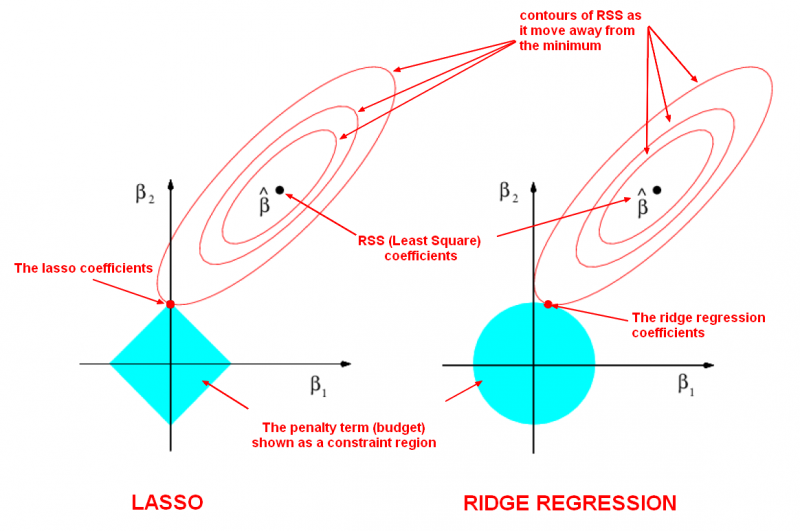
\includegraphics[scale=0.5]{Chap8-ChoixModeleRLM/Figures/lasso_vs_ridge_regression}
\caption[Illustration de la différence entre le LASSO et la régression ridge.]{Illustration de la différence entre le LASSO et la régression ridge. \\{\footnotesize Source : \url{http://gerardnico.com/wiki/data_mining/lasso}}}
\label{fig:lasso}
\end{figure}

\newpage

Tel qu'indiqué plus haut, il faut choisir le paramètre $\lambda$ pour obtenir une estimation avec le LASSO. Celui-ci est généralement choisi pour minimiser l'erreur de prévision, telle qu'estimée par une méthode comme la validation croisée.

Notons que sous certaines hypothèses, on peut montrer que le LASSO identifie correctement les coefficients qui ne valent pas 0 avec une grande probabilité. Toutefois, les estimateurs sont en général biaisés vers 0, et pas nécessairement convergents. En pratique, on utilise donc parfois le LASSO pour faire une sélection de variables, et on estime ensuite les coefficients avec la méthode des moindres carrés sans pénalité.

Enfin, un autre avantage de la régression LASSO est qu'elle permet d'ajuster un modèle dans le cas où le nombre de paramètres à estimer $p'$ est supérieur au nombre d'observations $n$.

\newpage

\section{Le cas des variables catégoriques et interactions}

Dans le cas de modèles de régression contenant des variables catégoriques et des interactions, il faut être un peu plus prudent dans la sélection de modèle.

\subsection{Sélection de modèle avec variables catégoriques}

La sélection se fait comme à l'habitude en présence de variables dichotomiques.

Avec des variables polytomiques, la règle utilisée en sélection de modèle, quel que soit le
critère de sélection, est que les $\beta$ correspondant à une m\^eme variable polytomique soient ou bien tous exclus du modèle, ou bien tous inclus dans le modèle. On peut aussi décider de fusionner certaines catégories de la variable polytomique si c'est suggéré par la forme du modèle sélectionné.

\begin{exemple}
Considérons de nouveau l'exemple \ref{eg:lot}. Si un critère de sélection indique que le meilleur modèle est $Y_i=\beta_0+\beta_{11}x_{11i}+\beta_{13}x_{13i}+\varepsilon_i$, alors on ajoutera $\beta_{12}x_{12i}$ à ce modèle car $\beta_{11}$, $\beta_{12}$ et $\beta_{13}$ sont tous reliés à la variable \og lot \fg et doivent donc ou tous \^etre inclus dans le modèle, ou tous \^etre exclus du modèle, et comme au moins un
de ces $\beta$ semble important, nous les incluons tous. On pourrait aussi décider de fusionner les lots 1 et 2 pour créer une nouvelle variable à trois catégories.
\end{exemple}




\subsection{Sélection de modèle en présence d'interactions}

Si une interaction entre plusieurs variables exogènes est incluse
dans un modèle, on laisse en général les effets plus simples
correspondants dans le modèle. Ceci facilitera l'interprétation des différents coefficients du modèle.

\begin{exemple}
Supposons que le modèle complet est
$$Y=\beta_0+\beta_1x_{1}+\beta_2x_{2}+\beta_3x_{3}+
\beta_{12}x_{1}x_{2}+\beta_{13}x_{1}x_{3}+\beta_{23}x_{2}x_{3}+\varepsilon,$$
mais que les procédures de sélection de variables indiquent que seulement les coefficients $\beta_1$ et $\beta_{23}$
semblent importants.
Nous utiliserions alors le modèle
%$$Y_i=\beta_0+\beta_1x_{1i}+\beta_2x_{2i}+\beta_3x_{3i}+\beta_{23}x_{2i}x_{3i}+\varepsilon_i$$
$$Y=\beta_0+\beta_1x_{1}+\beta_2x_{2}+\beta_3x_{3}+\beta_{23}x_{2}x_{3}+\varepsilon$$
car avec la présence de $\beta_{23}$ dans le modèle, il est
recommandé d'y inclure $\beta_2$ et $\beta_3$.
\end{exemple} 

\chapter{Multicolinéarité}\label{sec:Multicolinéarité}
\minitoc \mtcskip \minilof




\section{Introduction et définition}
Depuis le début du cours, nous avons supposé que la matrice  $\boX$ est une matrice de plein rang, c'est-à-dire qu'il existe une unique inverse à la matrice $\boX'\boX$, et donc qu'il n'existe qu'un seul vecteur $\hbobeta$ qui minimise la somme des carrés résiduels $SC_{\text{res}}$. Toutefois, en pratique certaines colonnes de $\boX$ peuvent être reliées linéairement entre elles. C'est ce qu'on nomme la  multicolinéarité.

%Si certaines colonnes de $X$ sont reliées linéairement entre elles, alors cet inverse n'est plus unique et on ne peut aller plus %loin. Par contre, si certaines colonnes ne sont pas exactement liées de façon linéaire mais sont près de l'être, alors il est %quand même possible de trouver un unique estimateur $\hbobeta$.
La définition mathématique formelle de la multicolinéarité est la suivante.
\begin{defn}\label{def:multi}
Il y a \textbf{multicolinéarité exacte} lorsqu'une variable est la combinaison linéaire d'une ou de plusieurs autres variables, c'est-à-dire  lorsqu'il existe une
 combinaison de constantes $d_1,\ldots,d_p$ (pas toutes \'egales
 \`a z\'ero) telle que
 $$\sum_{j=1}^pd_jX_j=\boz.$$
\end{defn}

\begin{defn}
La \textbf{multicolinéarité} au sens large se produit lorsqu'il existe une
combinaison de constantes $d_1,\ldots,d_p$ (pas toutes \'egales
 \`a z\'ero) telle que
 $$\sum_{j=1}^pd_jX_j\approx \boz.$$
 \end{defn}
Dans le cas de multicolinéarité exacte, la matrice $\boX'\boX$ n'est pas inversible et les coefficients ne sont pas tous identifiables de façon unique. Les valeurs ajustées restent définies comme la projection de $\boY$ sur l'espace engendré par les colonnes de $\boX$.
La multicolinéarité exacte ne représente pas un problème : elle se détecte facilement et il suffit d'enlever la ou les variables en cause pour régler le problème.
La multicolinéarité au sens large est plus fréquente et plus difficile à détecter.

La multicolinéarité au sens large pose plusieurs problèmes :
\begin{enumerate}
  \item Instabilité de $(\boX'\boX)^{-1}$, ce qui entraîne qu'une petite variation en $\boY$ peut se traduire par de très grands changements en $\hbobeta$. Les valeurs ajustées aux profils observés peuvent toutefois rester stables.
  \item On observe des $\hat{\beta}_i$ de signe inattendu ou contre-intuitif.
  \item Les variances de certains $\hat{\beta}_i$ peuvent être grandes. Les prédictions à des profils éloignés du domaine observé peuvent également être peu précises.
  \item Les méthodes de sélection de variables ne concordent pas.
  \item Certains paramètres peuvent se révéler non-significatifs alors que la corrélation des variables correspondantes avec $Y$ est très grande.
\end{enumerate}

Le problème, au fond, est que les variables s'expliquent entre elles. Si on s'imagine l'espace d'une régression à deux variables, c'est comme si les points étaient alignés en «piquets de clôture». Ce phénomène n'est pas facile à détecter dans un espace à haute dimension. Nous présenterons ici quelques outils de détection de la multicolinéarité.

\section{Détection de la multicolinéarité}
\subsection{La matrice de corrélations}
À première vue, on pourrait être tenté de calculer la matrice des corrélations entre les variables exogènes pour détecter la multicolinéarité.

Le coefficient de corrélation échantillonnal entre la variable $x_j$ et la variable $x_k$ est donné par
$$r_{jk}=\dfrac{1}{n-1}\sum_{i=1}^n\frac{(x_{ji}-\overline x_j)(x_{ki}-\overline x_k)}{s_js_k}, \;j\in\{1,\ldots,p\},k\in\{1,\ldots,p\}$$
où $\overline x_j=\sum_{i=1}^n x_{ji}/n$ et $s_j=\sqrt{\sum_{i=1}^n(x_{ji}-\overline x_j)^2/(n-1)}$, et de même pour $\overline x_k$ et $s_k$.

On peut aussi écrire la matrice des coefficients de corrélation échantillonnaux (en excluant la colonne de 1) comme
\begin{eqnarray*}
\boX_c^{*'}\boX_c^{*}=\left(\begin{array}{cccc}
1 & r_{12} &  \cdots & r_{1p} \\
r_{21} & 1 & \cdots & r_{2p} \\
\vdots & \vdots & \ddots  & \vdots \\
r_{p1} & r_{p2} & \cdots  & 1
\end{array}
\right)
\end{eqnarray*}
où $$\boX_c^*=\left(\frac{\bo{x}_1-\overline{\bo{x}}_1}{\sqrt{\sum_i (x_{1i}-\overline x_1)^2} }\;\;\frac{\bo{x}_2-\overline{\bo{x}}_2}{\sqrt{\sum_i (x_{2i}-\overline x_2)^2}} \ldots \frac{\bo{x}_p-\overline{\bo{x}}_p}{\sqrt{\sum_i (x_{pi}-\overline x_p)^2}}  \right)\quad \text{ et } \quad \overline{\bo{x}}_j=(\overline x_j,\ldots,\overline x_j)'.$$



Si deux variables exogènes sont linéairement reliées, leur coefficient de corrélation devrait
être élevé. Cependant deux problèmes majeurs empêchent les coefficients de corrélation
d'être des bons outils de diagnostic:
\begin{itemize}
\item[(i)] il est difficile de dire ce qu'est une grande valeur de la corrélation
\item[(ii)] la multicolinéarité est souvent induite par une dépendance linéaire entre plus de deux variables.
\end{itemize}
Pour voir que le point (ii) constitue un
problème, il est possible de créer des exemples où $p$ variables sont parfaitement linéairement
dépendantes, mais où les coefficients de corrélation de toutes les paires de variables sont
égaux en valeur absolue à $1/(p-1)$. Ainsi, même si la corrélation entre deux variables est indésirable, cela
ne représente qu'un cas particulier de la multicolinéarité.

\subsection{Le facteur d'inflation de la variance (VIF)}
\label{sec:vif}
Une approche plus sensible consiste à évaluer le degré de dépendance linéaire de chaque
variable exogène sur les autres variables exogènes. Ainsi pour la $j^e$ variable exogène,
on peut mesurer ce niveau de dépendance en effectuant une régression linéaire avec la $j^e$
variable exogène comme variable réponse et les $p-1$ variables exogènes restantes comme variables explicatives. Le coefficient de détermination de cette régression, noté $R^2_j$, mesurera la proportion de la variabilité de la $j^e$ variable exogène qui est expliquée de fa\c{c}on linéaire par les autres variables exogènes. Si $R_j^2$ est grand, on a vraisemblablement un problème.

Cette idée se matérialise dans le facteur d'inflation de la variance (en anglais, VIF pour Variance Inflation Factor). Celui-ci est défini de la façon suivante :
\begin{eqnarray}
  \mbox{VIF}_j &=& \frac{1}{1-R_j^2}
\end{eqnarray}
Si $R_j^2\rightarrow 1$, alors $VIF_j\rightarrow \infty$. Ainsi, une grande valeur de $\mbox{VIF}_j$ signifie une valeur proche de 1 de $R_j^2$, et donc une forte dépendance linéaire des variables exogènes.

Le nom \og facteur d'inflation de la variance \fg  $\;$ vient du fait que la variance de $\hat{\beta}_j$ s'exprime en fonction du VIF comme suit :
\begin{eqnarray*}
% \nonumber to remove numbering (before each equation)
  \var[\hat{\beta}_j] &=& \frac{\sigma^2}{(\boX'\boX)_{jj}} \mbox{VIF}_j
\end{eqnarray*}
On voit donc l'effet de cette multicolinéarité sur la variance des estimateurs des coefficients.

 Plusieurs
auteurs suggèrent un VIF > 10 comme point où l'on doit commencer à considérer la présence
de multicolinéarité aux conséquences importantes. Cependant, les VIF à eux seuls ne sont
pas un diagnostic complet. Parmi les points faibles des VIF on dénote
\begin{itemize}
\item [(i)]l'incapacité de détecter des multicolinéarités impliquant la colonne de 1 de la matrice d'incidence
\item [(ii)] l'incapacité de cerner le nombre de quasi dépendances linéaires présentes dans les données
\item [(iii)] le fait qu'on a jamais réussi à cerner une valeur précise pour le VIF où l'on doit vraiment commencer à s'inquiéter (10 est une valeur \textit{ ad hoc}).
\end{itemize}

\begin{remarque}
Une mesure équivalente au facteur d'inflation de la variance est la tolérance définie comme suit :
$$\mbox{TOL}_j=1-R_j^2=1/\mbox{VIF}_j.$$
La tolérance $\mbox{TOL}_j$ est donc la partie de la variabilité dans la j$^{\text{ème}}$ variable exogène qui n'est pas expliquée par les autres variables exogènes. Ainsi, si on définit un cas problématique comme un cas où $\mbox{VIF}>10$, ceci est équivalent à définir les cas problématiques comme ceux ayant une $\mbox{TOL}< 10 \%$, c'est-à-dire ceux pour qui au moins 90 \% de la variabilité est expliquée par les autres variables exogènes.
\end{remarque}

\subsection{L'indice de conditionnement}

\label{sec:FacteurDeConditionnement}
L'approche la plus efficace afin de détecter les causes de multicolinéarité est basée sur les valeurs propres de la matrice des coefficients de corrélation échantillonnaux $\boX_c^{*'}\boX_c^*$, ou sur la matrice des valeurs réduites, mais non centrées $\boX^*$ (qui permet l'inclusion de la colonne de 1), où 

$$\boX^*=\left(\frac{\bo{x}_1}{\sqrt{\sum_i x_{1i}^2} }\;\;\frac{\bo{x}_2}{\sqrt{\sum_i x_{2i}^2}} \ldots \frac{\bo{x}_p}{\sqrt{\sum_i x_{pi}^2}}  \right).$$

En se servant de la décomposition en valeurs propres de $\boX^{*'}\boX^*$, i.e.
$$\boX^{*'}\boX^*=\bo{P}\bo{\Lambda} \bo{P}'$$
avec $\bo{\Lambda}=\text{diag}(\lambda_1,\ldots,\lambda_{p'})$ et $\bo{P}\bo{P}'= \bo{P}'\bo{P}=\bo{I}_{p'}$, on peut alors montrer que
\begin{equation}
\text{tr}(\boX^{*'}\boX^*)=\text{tr}(\bo{P}\bo{\Lambda} \bo{P}')=\mbox{tr}(\bo{P}'\bo{P}\bo{\Lambda})=\mbox{tr}(\bo{\Lambda})=\sum_{j=1}^{p'}\lambda_j=p'.
\label{eq:traceIC}
\end{equation}
En présence de multicolinéarité, le déterminant de $\boX^{*'}\boX^*$, qui est égal à $\prod\limits_{j=1}^{p'}\lambda_j$, aura une valeur proche de 0.



Ainsi, en présence de multicolinéarité l'équation \ref{eq:traceIC} indique que la somme des valeurs propres doit être égale à $p'$, mais que leur produit sera proche de 0. Puisque les valeurs propres sont toutes positives, cela implique qu'en présence de multicolinéarité, il y aura \`a la fois des valeurs propres de grandes et de faibles valeurs. Le nombre de valeurs propres proches de zéro indique le nombre de directions presque linéairement dépendantes. Dans cette situation, le rapport de la plus grande valeur propre sur la plus faible sera donc élevé.

Les \textbf{indices de conditionnement} notés $\eta_j$ pour ${j=1,2,\cdots,p'}$ sont définis comme les racines carrées des rapports entre la plus grande valeur propre de la matrice $\boX^{*'}\boX^*$ et chacune de ses autres valeurs propres, c'est-à-dire
$$\eta_j=\sqrt{\frac{\lambda_{max}}{\lambda_j}}.$$

Plusieurs auteurs semblent s'entendre pour dire qu'une valeur de $\eta_j > 30$ indique une multicolinéarité dont il faut se
soucier.

La plus grande valeur de $\eta_j$ est égale à
$$\kappa=\sqrt{\frac{\lambda_{max}}{\lambda_{min}}}.$$

$\kappa$ est parfois appelée \textbf{ facteur de conditionnement}.


%Les valeurs propres $\lambda_1, ..., \lambda_{p'}$ de $(\boX^'\boX)^{-1}$ sont réelles et positives. On peut écrire $(\boX'\boX)=\bo{P}\bo{\Lambda} \bo{P}'$ où $\bo{P}$ est la matrice orthogonale des vecteurs propres et $\bo{Lambda}$ est la matrice diagonale des valeurs propres de $(\boX'\boX)$.
%
%Il y a multicolinéarité lorsque $\lambda_{p'}$, la plus petite valeur propre de $\boX'\boX$, est proche de 0. Rappelons que le déterminant de $\mbox{det}(\boX'\boX)= \prod_{i=1}^{p'} \lambda_{i}=0$ lorsque $\lambda_{p'}=0$. Donc, si $\lambda_{p'}\cong 0$, $(\boX^'\boX)^{-1}$ est instable numériquement.
%
%
% à continuer ici. vérifier la définition du facteur de conditionnement.
%

%Le facteur de conditionnement est un indicateur de la multicolinéarité qui utilise les valeurs propres de la matrice $(\boX^{*'}\boX^*)$. On  le définit de la façon suivante:
%\begin{eqnarray}
%% \nonumber to remove numbering (before each equation)
%  \kappa &=& \sqrt{\frac{\lambda_{\text{max}}}{\lambda_{\text{min}}}}.
%\end{eqnarray}
%Bien que ceci n'ait pas de véritable fondement, on considère généralement un $\kappa>30$ comme étant problématique.

Soit $\bo{p}_j$, le vecteur propre correspondant à la valeur propre $\lambda_j$.
%Les éléments de ces vecteurs peuvent nous aider à identifier le nombre de quasi dépendances linéaires dans les données, et quelles variables exogènes font partie de chaque quasi dépendance. En effet,
Pour les coefficients associés aux colonnes normalisées,
$$\var[\hat\beta_{k-1}]=\sigma^2(\bo{X}^{*'}\bo{X}^*)^{-1}_{kk}=\sigma^2\sum_{j=1}^{p'}p_{kj}^2/\lambda_j,$$
la portion de variance de $\hat\beta_{k-1}$ expliquée par la $j^{e}$ dépendance linéaire peut se mesurer comme suit :
$$v_{kj}=\frac{p_{kj}^2/\lambda_j}{\sum\limits_{l=1}^{p'}p_{kl}^2/\lambda_l}.$$

Pour détecter la multicolinéarité on suit donc la procédure suivante:
\begin{enumerate}
\item Calculer les indices de conditionnement $\eta_j$ et vérifier si certains d'entre eux possèdent une valeur supérieure à 30.
\item Pour chaque $\eta_j$ dont la valeur excède 30, calculer les proportions de la variance $v_{1j},v_{2j},\cdots,v_{p'j}$.
\item Les variables exogènes correspondant aux coefficents avec des valeurs de $v_{kj}$ élevées (en général nettement supérieures à 60 \%) sont multicolinéaires.
\end{enumerate}

\section{Les solutions possibles à la multicolinéarité}
\label{sec:solutionsMulticolinearite}

La solution la plus simple est de retirer une ou plusieurs variables exogènes. Typiquement, on retranchera les variables ayant le plus grand VIF, une à la fois. Dans la pratique, ce retrait des variables doit se faire en collaboration étroite avec le client, car dans le choix des variables, c'est d'abord l'interprétation qui compte. Il est parfois possible  de combiner des variables exogènes redondantes, par exemple pour calculer un score à partir de plusieurs variables exogènes.

Quelques autres solutions sont également disponibles.



\subsection{La régression \og ridge \fg}

La régression ridge, présentée à la section \ref{sec:ridge} peut également être utilisée en cas de multicolinéarité, mais donne des estimateurs biaisés. Le paramètre de pénalisation se choisit, par exemple, par validation croisée.


\subsection{La régression basée sur les composantes principales}


On peut également faire une régression sur les composantes principales de la matrice d'incidence. Les facteurs dans une analyse en composantes principales sont donnés par les colonnes de la matrice $\bo{F}$ suivante :
$\bo{F}=\boX^*\bo{P}$,
où $\bo{P}$ est la matrice des vecteurs propres de $\boX^{*'}\boX^*$. Cette matrice est telle que $\bo{P}'\bo{P}=\bo{P}\bo{P}'=\boI$. En utilisant cette propriété matricielle, nous pouvons écrire le modèle de régression multiple comme
\begin{eqnarray*}
\boY & = & \beta_0\bo{1}+\boX^*\bobeta + \boeps \\
 & = & \beta_0\bo{1}+\boX^*\bo{P}\bo{P}'\bobeta+ \boeps\\
& = & \beta_0\bo{1}+\bo{F}\bo{\gamma}+\boeps,
\end{eqnarray*}
où $\bo{\gamma}=\bo{P}'\bobeta$ ou encore $\bobeta=\bo{P}\bo{\gamma}$. Le théorème de Gauss-Markov implique que $\hbobeta=\bo{P}\hat{\bo{\gamma}}.$
La multicolinéarité n'est plus présente, mais au prix d'un biais dans les estimateurs. Ce biais est présent si on ne retient dans la modélisation que les facteurs associés aux plus grandes valeurs propres de $\boX^{*'}\boX^*$.

Le principal problème de la régression en composantes principales est son interprétation, qui peut être hasardeuse. %On peut se rattraper en calculant $\hbobeta=\bo{P}\hat{\bo{\gamma}},$ cependant dans ce cas $\esp[\hbobeta]\neq\bobeta$. L'estimation est biaisée.

%Enfin, on peut faire une régression en composantes principales. Pour ce faire, on commence par centrer-réduire la matrice X, on obtient $X^*$. On calcule ensuite la matrice des corrélation $X^{*T}X^*$. On trouve les valeurs propres de cette matrice et on effectue la régression avec le modèle suivant:
%\begin{eqnarray}
%% \nonumber to remove numbering (before each equation)
%  Y &=& Z\alpha + \epsilon
%\end{eqnarray}
%où $Z=X^*P^T$ et $\alpha=P\beta$. On ne retient que le nombre de composantes nécessaires.
%
%Le principal problème de la régression en composantes principales est son interprétation, qui peut être hasardeuse. On peut se rattraper en calculant $\hat{\beta}=P\hat{\alpha}$, mais dans ce cas $E[\hat{\beta}]\neq\beta$; l'estimation est biaisée.



\chapter{Observations aberrantes et influentes}\label{sec:DonneesInfluentes}
\minitoc \mtcskip \minilof




\vspace{-0.1in}
%Tout comme on a sélectionné les variables à inclure dans le modèle de RLM, il peut être nécessaire de sélectionner les observations à inclure dans le modèle.
On doit examiner les observations qui influencent fortement l'estimation des paramètres et documenter leur effet par une analyse de sensibilité. Avant de parler plus en détails de ces données influentes, il faut bien définir deux termes importants.

\begin{defn}\label{def:aber}
Une observation est \textbf{ aberrante} si elle ne cadre pas avec le modèle.
\end{defn}

\vspace{-0.1in}
Ce sera donc une observation qui a un résidu de grande taille. Une donnée aberrante n'est pas problématique en elle-même, mais elle peut indiquer une erreur dans la valeur d'une variable exogène ou de la variable endogène.

\begin{defn}\label{def:infl}
Une donnée \textbf{influente} est une observation qui, \`a elle seule, peut avoir un impact sérieux sur les conclusions d'une analyse de régression.
\end{defn}

\vspace{-0.1 in}
Parmi les exemples \og d'impact sérieux \fg, on peut citer des $\hat{\beta}$ négatifs quand on sait qu'ils devraient \^etre positifs (ou vice-versa) ou encore une variable exogène qui devrait \^etre importante mais qui est considérée non significative. Une ou des observations influentes peut également diminuer le pouvoir prédictif du modèle.

%\newpage
\section{Sources de l'influence}

L'influence d'une observation provient souvent d'une combinaison de
deux sources :
\begin{description}
\item[Source 1:] L'observation a un grand levier, c'est-à-dire qu'elle a une grande capacité \textit{a priori} à influencer les résultats de la régression.
\item[Source 2:] L'observation a une valeur extrême de $Y$ par rapport au modèle.
%Donnée ayant une erreur produisant une valeur extr\^eme de $Y$.
\end{description}
On peut facilement identifier les observations avec ces deux caractéristiques.

\textbf{Levier d'une observation}

Une observation a un grand levier si sa valeur de $\boldx_i$ est loin du centre (centro\"{\i}de) de toutes les observations. La distance entre une observation et le centro\"{\i}de de toutes les autres peut être calculée facilement à partir de la matrice d'incidence $\boX$. Plus précisément, le levier de la $i^e$ observation est le $i^e$ élément diagonal de la matrice chapeau $\boH=\boX(\boX'\boX)^{-1}\boX'$, qui peut s'exprimer comme
$h_{ii}=\boldx_i'(\boX'\boX)^{-1}\boldx_i$.

Qu'est-ce qu'une grande valeur de $h_{ii}$? Il est difficile de
répondre \`a cette question de fa\c{c}on générale. Cependant nous
savons que tr$(\boH)=\sum_{i=1}^n h_{ii}=p'$, o\`u $p'$ est le nombre
de paramètres dans le modèle. Donc un $h_{ii}$ moyen prend une valeur de $p'/n$
et un $h_{ii}$ qui se démarque nettement de cette valeur
signifie une donnée \`a grand levier. \citet{Bel_Kuh_Wel:80} suggèrent de retenir les valeurs de $h_{ii}>2p'/n$.

\textbf{Observation extrême}

Une observation est extrême (ou aberrante) par rapport au modèle si son résidu est grand. On regardera plus précisément le résidu studentisé. On rappelle que celui-ci est donné par

En notant $p'$ le nombre de coefficients, incluant l'ordonnée à l'origine,
\[
 s_{(i)}^2=\frac{(n-p')\hat\sigma^2-\hat\varepsilon_i^2/(1-h_{ii})}{n-p'-1},
 \qquad T_i=\frac{\hat\varepsilon_i}{s_{(i)}\sqrt{1-h_{ii}}}.
\]
Sous les postulats normaux et si le modèle privé de l'observation $i$ reste de
plein rang, $T_i\sim\mathcal{T}_{n-p'-1}$. Un repère exploratoire courant est
$|T_i|>2$. Pour un dépistage simultané au seuil $\alpha$, on peut comparer
$|T_i|$ à $t_{n-p'-1;1-\alpha/(2n)}$. Ces repères ne constituent pas des
règles automatiques de retrait.

\begin{remarque}
Avoir un grand levier et être une observation extrême sont des indices qu'une observation pourrait avoir une influence démesurée sur les résultats de la régression. Pour tester si cela est effectivement le cas, on doit mesurer directement l'influence de l'observation sur la régression. Il est important de comprendre qu'une donnée avec un grand levier peut ne pas être influente. Il en est de même pour une observation extrême.
\end{remarque}


%Un grand levier n'implique pas nécessairement une influence. Tout diagnostic d'influence doit \^etre basé sur une combinaison de $h_{ii}$ et $R_{i}$.

\section{Mesures d'influence}

Pour mesurer si une donnée est influente ou non, on évalue son impact sur la prévision $\hY$ et sur l'estimation de $\bobeta$. Les différentes statistiques utilisées sont présentées ici.

\subsection{Influence sur la prévision}
La statistique suivante mesure l'influence de la $i^e$ donnée
dans la prévision $\hat{Y}_i$ de $Y_i$ (\textit{Difference in Fit}) :
$$DFFIT_i={\hat{Y}_i-\hat{Y}_{i,-i}\over
\hat\sigma_{-i}\sqrt{h_{ii}}}=T_i\sqrt{h_{ii}\over1-h_{ii}},$$ o\`u
$\hat{Y}_{i,-i}$ désigne la valeur de la prévision de $Y_i$ basée
sur un jeu de données qui ne contient pas la $i^e$ donnée,
c'est-à-dire $\hat{Y}_{i,-i}=\boldx_i'\hat{\bobeta}_{-i}$.

Il faut se rappeler ici que $\var[\hat Y_i]=\sigma^2h_{ii}$. Les différences au numérateur de $DFFIT_i$ sont donc standardisées de sorte qu'elles s'expriment en multiples de l'écart-type de la prévision.

Nous analysons les $DFFIT_i$ de la m\^eme fa\c{c}on que nous nous penchons sur les $T_i$, c'est-à-dire que des grandes valeurs de $|DFFIT_i|$ constituent un signe que la $i^e$ donnée possède une grande influence sur la valeur de la prévision. \citet{Bel_Kuh_Wel:80} indiquent qu'il faut retenir les valeurs de $|DFFIT_i|>2\sqrt{p'/n}$ alors que d'autres statisticiens proposent simplement de retenir les valeurs de $|DFFIT_i|>2$.

\subsection{Influence sur les estimations des paramètres}
La statistique suivante mesure l'influence de la $i^e$
observation sur la valeur de l'estimateur de $\beta_j$ (\textit{ Difference in Beta}):
$$DFBETAS_{ji}={\hat{\beta}_j-\hat{\beta}_{j,-i}\over
\hat\sigma_{-i}\sqrt{(\boX'\boX)^{-1}_{jj}}}.$$
Il faut se souvenir ici que $\var[\hat\beta_j]=\sigma^2(\boX'\boX)^{-1}_{jj}$. Les différences au numérateur de la statistique sont  à nouveau standardisées.
Encore une fois, les grandes valeurs de $DFBETAS_{ji}$ indiquent que la $i^e$ donnée possède une grande influence sur l'estimation de $\beta_j$. \citet{Bel_Kuh_Wel:80} proposent de considérer les valeurs de $|DFBETAS_{ji}|>2/\sqrt{n}$ alors que d'autres statisticiens suggèrent simplement de retenir les valeurs de $|DFBETAS_{ji}|>2$. \\

Le signe de $DFBETAS_{ji}$ est un bon indicateur. En effet, si un certain $\hat\beta_j$ est négatif alors qu'on se serait attendu à une valeur positive, alors un $DFBETAS_{ji}$ très négatif indique que le \og coupable \fg pourrait être l'observation $i$.

Comme nous obtenons $p\prime$ valeurs de $DFBETAS$
pour chaque observation, cette mesure devient peu pratique lorsque
nous sommes en présence d'un jeu de données ayant plusieurs
variables exogènes. Pour simplifier la recherche de valeurs influentes, Dennis Cook a proposé la statistique suivante, appelée distance
de Cook, qui permet de combiner les $DFBETAS$ d'une m\^eme observation:
\begin{eqnarray*}
\text{distance de Cook}_i\;=\;C_i & = & {(\hat{\bobeta}-\hat{\bobeta}_{-i})'(\boX'\boX)(\hat{\bobeta}-\hat{\bobeta}_{-i})
\over p' \hat\sigma^2} \\
& = & \frac{\sum_{k=1}^n(\hat Y_k-\bo{x}_k'\hat{\bobeta}_{-i})^2}{p'\hat\sigma^2} \\
& = & \frac{\hat\varepsilon_i^2}{(1-h_{ii})^2}\frac{h_{ii}}{\hat\sigma^2 p'} \\
% & = & \frac{\hat\varepsilon_{i,-i}^2}{p}\frac{h_{ii}}{1-h_{ii}}
\end{eqnarray*}
 Une grande valeur de $C_i$ indique une observation
ayant une influence prépondérante sur les $\beta$. \citet{Fox:91} suggère de porter notre attention sur les valeurs de $C_i>\frac{4}{n-p'}$. Il s'agit par la suite
d'examiner les $DFBETAS$ pour cette observation pour savoir quel(s)
$\hat\beta$ est (sont) affecté(s).


\subsection{Influence sur la performance des estimateurs}
Une donnée peut aussi avoir un impact néfaste sur la variance des estimateurs. Soit $||Var(\hat{\bobeta})|| = (\sigma^2)^{p'}||(\boX'\boX)^{-1}||$, le déterminant de la matrice de variance de $\hat{\bobeta}$, parfois appelé variance généralisée. L'influence de la $i^e$ donnée sur la variance de $\hat{\bobeta}$ peut \^etre calculée comme suit:

\begin{eqnarray*}COVRATIO_i&=&{||(\boX_{-i}'\boX_{-i})^{-1}\hat\sigma_{-i}^2||
\over||(\boX'\boX)^{-1}\hat\sigma^2||}\\
&=&\left({\hat\sigma_{-i}^{2}\over
\hat\sigma^{2}}\right)^{p'}\frac{1}{1-h_{ii}}.\end{eqnarray*}
Comme la seconde ligne l'illustre, une donnée possédant beaucoup de levier
donnera en général un $COVRATIO>1$, et une donnée aberrante un $COVRATIO<1$.

\citet{Bel_Kuh_Wel:80} proposent de porter notre attention sur les valeurs telles que
$|COVRATIO-1|~>~3p'/n$, c'est-à-dire sur les observations telles que\\ $COVRATIO~<~1~-~3p'/n$ ou $COVRATIO>1+3p'/n$.



\section{Que faire avec les données influentes?}
Si une donnée est influente, il faut prendre tous les moyens
possibles pour essayer de comprendre comment cette donnée a été
obtenue et s'assurer qu'il n'y a pas d'erreur qui aurait pu
survenir lors de la mesure, collecte ou saisie des données.

Si l'influence provient d'un grand
levier, alors il serait souhaitable d'aller chercher d'autres
données afin de combler le vide entre le centro\"{\i}de des
données et la donnée influente.

En général, on doit s'abstenir d'éliminer les données
influentes d'un jeu de données. Quelques exceptions:
\begin{itemize}
\item Erreur de mesure ou  de  saisie (corriger la donnée
est préférable \`a son élimination). \item Valeurs
mesurées scientifiquement peu plausibles. \item Donnée très
peu représentative du reste des données et de la population en
général. \end{itemize}

Il est \`a noter que souvent, une transformation de variable peut
grandement réduire l'influence de certaines données. 

\chapter{Techniques plus avancées}\label{sec:TechniquesAvancees}
\minitoc \mtcskip \minilof



On présente ici quelques techniques de régression plus avancées. Elles peuvent entre autres être utilisées si les postulats de la RLM ne sont pas vérifiés.


\section{Régression polynomiale}
\label{sec:regpoly}

L'idée derrière la régression linéaire est que le modèle
linéaire est une bonne approximation de la \og vraie \fg relation
entre la variable endogène et les variables exogènes
$$Y=f(x_1,x_2,\ldots,x_k)+\varepsilon.$$
Dans plusieurs cas, le modèle de régression linéaire sera
une approximation suffisamment bonne de $f(x_1,\ldots,x_k)$. Par
contre dans certaines situations, il arrive que l'approximation
linéaire ne soit pas assez proche de $f(x_1,\ldots,x_k)$ pour
donner un modèle approprié. Dans ces cas, nous pouvons
utiliser le principe disant que la plupart des fonctions peuvent
\^etre approchées aussi bien que l'on veut par une expansion
polynomiale. Plus il y a de la \og courbure \fg dans
$f(x_1,\ldots,x_k)$, plus le polyn\^ome utilisé pour
approcher $f(x_1,\ldots,x_k)$ doit \^etre de degré élevé
pour que l'approximation soit suffisamment précise.

En régression, ceci se traduit par le résultat suivant:
\begin{eqnarray*}
Y_i&=&f(x_{1i},\ldots,x_{ki})+\varepsilon_i\\
&\approx&\beta_0+\beta_1x_{1i}+\cdots+\beta_kx_{ki}\\
&\ &\ \ \ +\beta_{11}x_{1i}^2+\cdots+\beta_{kk}x_{ki}^2+
\beta_{12}x_{1i}x_{2i}+\cdots+\beta_{k-1,k}x_{k-1,i}x_{ki}\\
&\ & \ \ \ +\beta_{111}x_{1i}^3+\cdots+ \beta_{kk\cdots
k}x_{ki}^d+\cdots+\varepsilon_i.
\end{eqnarray*}
En général, il est rarement nécessaire de dépasser un modèle du second degré:
\begin{eqnarray*}
Y_i&=&\beta_0+\beta_1x_{1i}+\cdots+\beta_kx_{ki}\\
&\ &\ \ \ +\beta_{11}x_{1i}^2+\cdots+\beta_{kk}x_{ki}^2+
\beta_{12}x_{1i}x_{2i}+\cdots+\beta_{k-1,k}x_{k-1,i}x_{ki}.
\end{eqnarray*}

Il est possible que l'on rencontre des problèmes numériques ou
de multicolinéarité quand on utilise des modèles polynomiaux. Si l'objectif est de trouver un modèle faisant de bonnes prédictions, ce n'est pas vraiment un problème. Si on veut vraiment interpréter les valeurs des coefficients de chaque terme, alors on peut travailler avec les variables exogènes standardisées, c'est-à-dire de
remplacer $x_{ji}$ par
$$x_{ji}^*=\frac{(x_{ji}-\bar{x}_j)}{s_j}$$

$ \mbox{ o\`u } \bar{x_j}=\sum_ix_{ji}/n \mbox{ et } s_j^2=\sum_i(x_{ji}-\bar{x}_j)^2/(n-1).$

\subsubsection*{Sélection de modèle}

Comme c'était le cas avec les interactions, si un terme de
degré $d$ est inclus dans le modèle, alors en général on
inclut les termes de degré inférieur \`a $d$.% composés des termes présents dans le terme de degré $d$ en question.


%\noindent\textbf{Note:} Il est préférable d'utiliser une transformation de $Y$ et/ou de certains des $x$ si cette transformation donne d'aussi bons résultats qu'un modèle polynomial avec moins de paramètres. Par exemple, $$\ln Y_i=\beta_0+\beta_1x_{1i}+\varepsilon_i$$ ou $$Y_i=\beta_0+\beta_1e^{x_{1i}}+\varepsilon_i$$ peut \^etre préférable \`a $$Y_i=\beta_0+\beta_1x_{1i}+\beta_2x_{1i}^2+\beta_3x_{3i}^3+\varepsilon_i.$$ Un examen des résidus et de la valeur des critères de sélection de modèle aident souvent \`a déterminer quel modèle est le plus approprié pour vos données.


\subsubsection*{Test de comparaison de modèle pour justifier un degré supérieur}

% Tout comme c'était le cas avec les termes d'interaction, des termes de degré supérieur peuvent \^etre ajoutés \`a un modèle afin d'en vérifier l'ajustement.

\begin{exemple}
Soit le modèle
$Y=\beta_0+\beta_1x_{1}+\beta_2x_{2}+\varepsilon.$

Ce modèle est-il aussi valide que celui contenant des termes de degré 2?
$$Y=\beta_0+\beta_1x_{1}+\beta_2x_{2}+\beta_{11}x_{1}^2
+\beta_{22}x_{2}^2+ \beta_{12}x_{1}x_{2}+\varepsilon.$$

Nous pouvons utiliser un test $F$ de comparaison de modèles pour les hypothèses\\
$H_0:\ \beta_{11}=\beta_{22}=\beta_{12}=0$ contre \\
$H_1:$ au moins un de ces $\beta$ diffère de 0. \\

Si nous ne rejetons pas $H_0$, les données ne montrent pas d'amélioration significative par ces termes de second degré; les autres diagnostics restent nécessaires. Si nous rejetons $H_0$, alors le modèle de premier degré n'est pas adéquat.\\

On aurait pu vérifier l'ajout d'un seul terme à la fois, car il est fort possible qu'une relation quadratique soit souhaitable en $x_1$ mais pas en $x_2$.
\end{exemple}


\newpage

\section{Régression non linéaire}


Si l'espérance de $Y$ (ou de $g(Y)$) n'est pas une fonction linéaire des paramètres inconnus, mais qu'on a une idée de la vraie relation entre $Y$ et les variables indépendantes, on peut néanmoins estimer les paramètres de cette relation non linéaire avec la méthode des moindres carrés. Il n'y a pas de solution analytique dans ce cas, mais des  méthodes numériques peuvent minimiser la somme des carrés des erreurs.

\begin{exemple}
Dans une expérience sur des rats, on trempe  des portions du ventricule auriculaire gauche dans une solution de chlorure de calcium, puis on stimule électriquement le tissu et on mesure la longueur du rétrécissement de la bandelette de tissu.
On s'intéresse à la relation entre
\begin{itemize}
\item[] x :  la concentration de chlorure de calcium (en mM)
\item[] Y : le changement de longueur de la bandelette en réaction au choc (en mm)
\end{itemize}
La figure \ref{fig:rat1} illustre les données. Il est clair qu'un modèle linéaire n'est pas approprié.

Il se trouve toutefois qu'on a déjà une idée du modèle approprié pour les données:
$$ Y_i =  \alpha + \beta e^{-x_i / \theta} + \varepsilon_i $$
La régression non linéaire permet d'estimer les coefficients par la méthode des moindres carrés. On trouve $\hat\theta = 0,6082$, $\hat\alpha = 28,9633$ et $\hat\beta = -34,2274$. La fonction de régression correspondante est également illustrée à la figure \ref{fig:rat1}.

\begin{figure}[H]
\centering
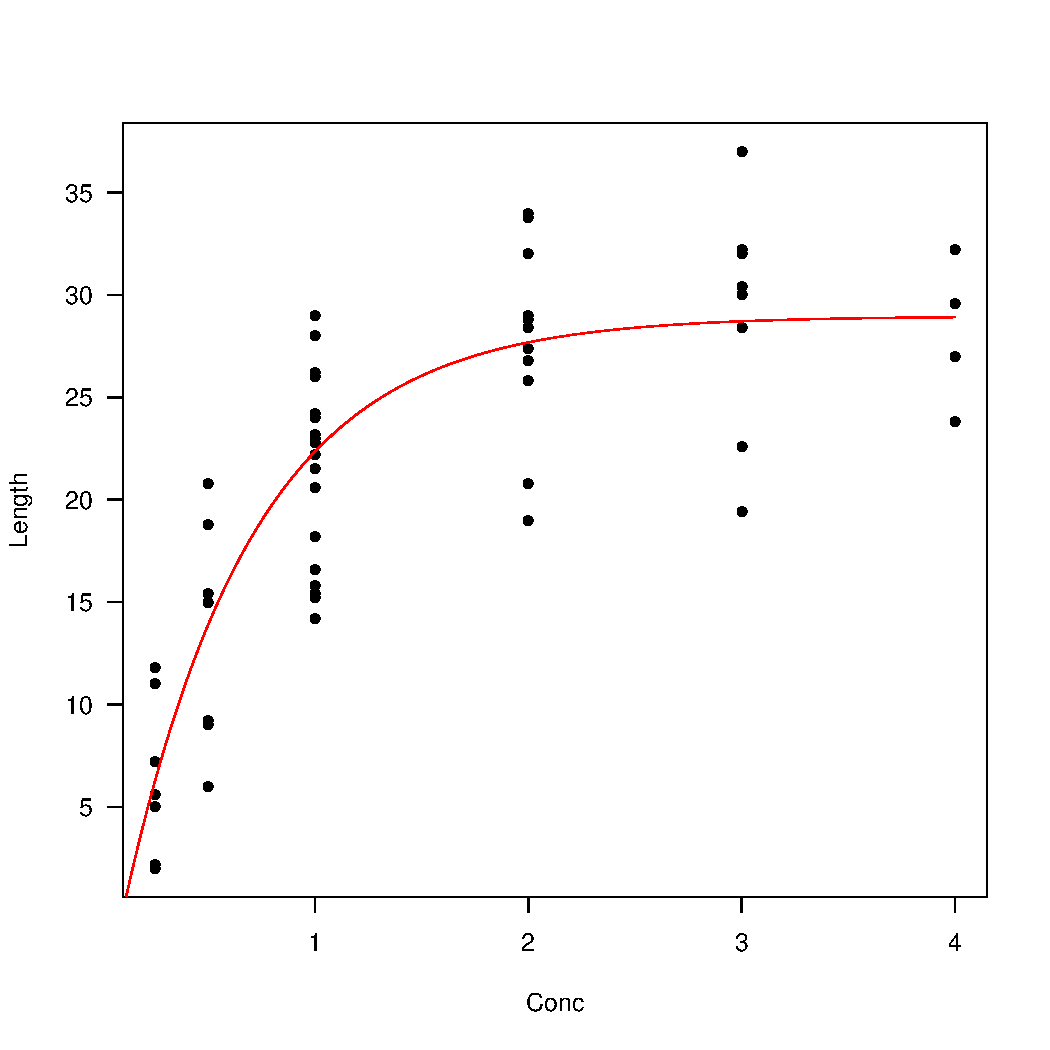
\includegraphics[scale=0.5]{Chap11-TechniquesAvancees/Figures/Nonlinear2}
\caption{Données d'une expérience sur des rats de laboratoire avec la fonction de régression estimée}
\label{fig:rat1}
\end{figure}
\end{exemple}


\newpage
\section{Régression pondérée}


La méthode des moindres carrés pondérés consiste \`a attribuer un poids différent  à chaque observation, et donc à trouver $\hat{\bobeta}$ tel que
$$\sum_{i=1}^nw_i(Y_i-\hat{Y}_i)^2$$
est minimale, o\`u $w_i$ est le poids associé à l'observation $i$.

Une application fréquente de la régression pondérée est lorsque l'hypothèse d'homo\-scédasticité n'est pas respectée, c'est-à-dire si le modèle est plutôt caractérisé par \\$\boeps\sim \mathcal{N}_n(\boz,\mbox{diag}(\sigma_1^2,\ldots,\sigma_n^2))$, o\`u les $\sigma_i^2$ ne sont pas nécessairement égaux.


Le choix des poids $w_i$ n'est pas toujours facile à faire. Si chaque observation est en réalité la moyenne de $n_i$ valeurs, on peut utiliser un poids égal $w_i=n_i$. Si la variance des erreurs est liée à une variable explicative, on peut faire un graphe des paires $(x_i,\, t_i)$, et voir
comment la variance des résidus studentisés évolue en
fonction de $x_i$. Si le graphe est en forme d'entonnoir ouvert
vers la droite, alors on pourra prendre $w_i=1/x_i$,
$w_i=1/\sqrt{x_i}$, $w_i=1/x_i^{2}$, etc. Si l'entonnoir ouvre vers
la gauche, alors on peut prendre $w_i=x_i$, $w_i=\sqrt{x_i}$,
$w_i=x_i^{2}$, etc. Il est toutefois recommandé d'essayer d'abord de régler le problème à l'aide d'une transformation de variable.

En régression linéaire multiple, il y a plusieurs variables explicatives, il faut donc trouver une stratégie plus globale en cas d'hétéroscédasticité. 
L'idéal serait d'identifier des poids de la forme $w_i\propto1/\sigma^2_i \;$, où $\sigma_i^2$ est la variance de l'erreur pour l'observation $i$. On peut démontrer que dans ce cas,
$$\hat{\bobeta}=(\boX'\boV^{-1}\boX)^{-1}\boX'\boV^{-1}\boY,$$
o\`u $\boV=\mbox{diag}(\sigma_1^2,\ldots,\sigma_n^2)$. La variance de
$\hat{\bobeta}$ est alors
\begin{eqnarray*}
\var(\hat{\bobeta})&=&(\boX'\boV^{-1}\boX)^{-1}\boX'\boV^{-1}\;\boV\;\boV^{-1}\boX(\boX'\boV^{-1}\boX)^{-1}\\
&=&(\boX'\boV^{-1}\boX)^{-1}.
\end{eqnarray*}
Si $\boV$ est connue, la statistique obtenue en divisant
$\hat\beta_j-c$ par son écart-type connu suit une loi normale standard sous
$H_0$. Si $\boV=\sigma^2\bo{W}^{-1}$ avec $\bo{W}$ connue et $\sigma^2$
inconnue, on estime $\sigma^2$ par
\[
 s_W^2=\frac{\sum_i w_i(Y_i-\hat Y_i)^2}{n-p'}.
\]
Sous normalité, la statistique
$(\hat\beta_j-c)/\{s_W\sqrt{(\boX'\bo{W}\boX)^{-1}_{jj}}\}$ suit alors
une loi de Student à $n-p'$ degrés de liberté. Si les poids sont estimés à
partir des mêmes données, ces résultats sont généralement approchés.

Or, établir des estimations des $\sigma_i$ n'est pas si évident.  Voici quelques pistes de solutions (il faut d'abord ajuster une régression du modèle complet et s'assurer que la linéarité est respectée):

\begin{itemize}
\item Si le graphique des $\hat\varepsilon_i$ en fonction des $\hat Y_i$ est en entonnoir, on ajuste une régression des $|\hat\varepsilon_i|$ sur les $\hat Y_i$. Les valeurs prédites de ce nouvel ajustement sont une estimation de $\sigma_i$. (Et les poids seront $w_i=1/\hat\sigma_i^2$).

\item Si le graphique des $\hat\varepsilon_i^2$ en fonction des $\hat Y_i$ montre une tendance à la hausse, on ajuste une régression des $\hat\varepsilon_i^2$ sur les $\hat Y_i$. Les valeurs prédites de ce nouvel ajustement sont une estimation de $\sigma_i^2$. (Et les poids seront $w_i=1/\hat\sigma_i^2$).
% Source: https://onlinecourses.science.psu.edu/stat501/node/352
\end{itemize}
%Parfois on utilise $\boV=\boV^*\sigma^2$ et on estime $\sigma^2$ par $$s^2={\sum_{i=1}^nw_i(Y_i-\hat{Y}_i)^2\over n-p'}.$$

% Une table d'analyse de variance peut aussi \^etre construite en utilisant la décomposition
% $$ {\underbrace{\boY'\boV^{-1}\boY}\atop SC_{tot:W}}={\underbrace{\hat{\bobeta}\boX'\boV^{-1}\boY} \atop SC_{reg:W}}+{\underbrace{(\boY-\boX\hat{\bobeta})'\boV^{-1}(\boY-\boX\hat{\bobeta})} \atop SC_{res:W}}.$$ 

Quelques remarques sur la régression pondérée:
\begin{itemize}
\item En général, les estimations des $\hat\beta_j$ ne seront pas dramatiquement changées par la régression pondérée.
\item Les degrés de liberté ne sont pas affectés par l'insertion de poids. %calculés de la m\^eme fa\c{c}on qu'en régression linéaire ordinaire.
\item Les intervalles de confiance et les tests d'hypothèses sont affectés par les poids.
% Source: https://onlinecourses.science.psu.edu/stat501/node/352
\end{itemize}

\newpage

\section{Modélisation de la dépendance}

Lorsque l'hypothèse d'indépendance des observations n'est pas vérifiée, on peut modéliser directement la dépendance en ajoutant des paramètres à la matrice de covariance des erreurs. Alors que la régression pondérée permet des valeurs différentes sur la diagonale de la matrice de covariance des erreurs, on modélise la dépendance en remplaçant les zéros hors diagonale par des paramètres à estimer. Selon la dépendance que l'on souhaite modéliser, on paramétrisera la matrice de covariance différemment.


Une forme particulière de dépendance est l'autocorrélation, qui arrive lorsque le résidu d'une observation est relié à celui de l'observation précédente, par exemple dans une série temporelle. Un modèle dit autorégressif peut alors être utilisé pour ajuster un modèle de régression.

Mathématiquement, on écrit
\begin{equation}\label{ar1}
\varepsilon_i=\rho\varepsilon_{i-1}+u_i, \end{equation} o\`u
les innovations $u_i$ sont i.i.d. $\mathcal{N}(0,\sigma_u^2)$. Le paramètre
$\rho$ dans (\ref{ar1}) est nommé paramètre
d'au\-to\-cor\-ré\-la\-tion, et sa valeur doit \^etre dans
l'intervalle (-1,1).

En supposant le processus stationnaire, avec $\varepsilon_1\sim\N(0,\sigma_u^2/(1-\rho^2))$ indépendant des innovations futures, à partir de (\ref{ar1}), nous pouvons
calculer directement que
\begin{eqnarray*}
\varepsilon_i&=&\sum_{j=0}^\infty\rho^ju_{i-j}\\
\esp[\varepsilon_i]&=&\sum_{j=0}^\infty\rho^j\esp[u_{i-j}]=0\\
\var[\varepsilon_i]&=&\sigma_u^2\sum_{j=0}^\infty\rho^{2j}={\sigma_u^2\over1-\rho^2}\\
\cov(\varepsilon_i,\varepsilon_{i+j})&=&\rho^{|j|}{\sigma_u^2\over1-\rho^2}.
\end{eqnarray*}
Comme on peut le voir, une autocorrélation positive entre
$\varepsilon_i$ et $\varepsilon_{i+1}$ est obtenue lorsque $\rho>0$,
tandis que $\rho<0$ donne une autocorrélation négative. Il n'y a
pas d'autocorrélation lorsque $\rho=0$.



%\section{Régression non-paramétrique}

\section{Autres}

Il existe plusieurs autres modèles de régression plus complexes, notamment la régression linéaire mixte, la régression linéaire locale, la régression non-paramétrique, les arbres de régression, etc. 

\bibliographystyle{2-stat-fr}
\bibliography{2-STT2100}
\end{document}
